% ===== INICIO DEL PREÁMBULO =====
%
\documentclass[msc,oneside]{udelar} % Poner msc para Maestría, dsc para Doctorado.

\usepackage[
acronyms, 											 % Utiliza el glosario de acronimos.
nohypertypes={acronym,notacion,simbolos,glosario},   % Quita los links en el texto al glosario.
nonumberlist,                                       % Quita los links en los glosarios al texto.
nogroupskip,                                         % Quita los espacios entre diferentes grupos dentro de un glosario.
nopostdot 											 % Quita el punto final en los acrónimos.
]{glossaries}



%Agrega número de lineas
%\usepackage{lineno}


\hypersetup{ colorlinks = true } % Hipervínculos: escribir "false" para imprimir o "true" para ver en digital.

% Cargar estilo bibliográfico copiando del documento "Estilos bibliográficos UdelaRTeX.pdf"

%%%%%%%%%BIBLOGRAFIA%%%%%%%%%%%%%%%%%%%%%%%%%%%%%%%%%%%%%%%%%%%%%%%%%%
%APA%%%%%%%%%
\usepackage[backend=biber,style=apa,sortcites,natbib=true]{biblatex}
\usepackage{estilos_bibliograficos/udelartex_apa}


%VANCOUVER%%%%%%%%%%
%\usepackage[backend=biber,style=numeric,sortcites,natbib=true,%
%terseinits=true,firstinits=true]{biblatex}
%\usepackage{estilos_bibliograficos/udelartex_vancouver}

%archivos .bib que se tengan para la bibliografía:
\addbibresource{bibliografia/AnalyticConductores.bib} % Agregar la cantidad de 
\addbibresource{bibliografia/Corrotacional.bib} % Se coloca una línea por archivo .bib.
\addbibresource{bibliografia/HistoriaCables.bib} % Se coloca una línea por archivo 
\addbibresource{bibliografia/SimuConductores.bib} % Se coloca una línea por archivo 
\addbibresource{bibliografia/TormentasConvectivas.bib} % Se coloca una línea por 
\addbibresource{bibliografia/MetodosNumericos_Softwares.bib}
\addbibresource{bibliografia/Filosofia.bib}
\addbibresource{bibliografia/Anexo.bib}
\loadglossary % No comentar esta línea

% A su vez, la clase udelar.cls ya tiene los siguientes paquetes cargados automáticamente, que podrían ser de interés saber para el usuario:
%{color},{hyphenat},{appendix},{lastpage},{babel},{inputenc},{amsmath,amssymb},{ifthen},{graphicx},{caption}{setspace},{tabularx},{eqparbox},{ltxcmds},{titletoc},{xcolor},{lineno},{xwatermark}

% Si se quieren agregar más paquetes, se recomienda colocarlos a partir de esta linea y antes de \begin{document}.
% ===========  INICIO PAQUETES ===============
\graphicspath{{./imagenes/ResultadosNumericos/RightAngeCantilever/},{./imagenes/ResultadosNumericos/SimpleCable/},{./imagenes/ResultadosNumericos/TransmissionTormenta/},{./imagenes/ResultadosNumericos/cantileverPendulum/}, {./imagenes/Preliminares/Corrotacional/},{./imagenes/Metodologia/},{./imagenes/Anexo/},{./imagenes/Introduccion/}}
% Paquetes adicionales
\usepackage{subfigure}
\usepackage{hyperref}
\usepackage{algorithm}
\usepackage{algorithmic}
\usepackage{multirow} 
\usepackage{multicol}
\usepackage{enumitem} 

\usepackage{listings}
\usepackage{xcolor}

\definecolor{codegreen}{rgb}{0,0.6,0}
\definecolor{codegray}{rgb}{0.5,0.5,0.5}
\definecolor{codepurple}{rgb}{0.58,0,0.82}
\definecolor{backcolour}{rgb}{0.95,0.95,0.92}

\lstdefinestyle{mystyle}{
	backgroundcolor=\color{backcolour},   
	commentstyle=\color{codegreen},
	keywordstyle=\color{magenta},
	numberstyle=\tiny\color{codegray},
	stringstyle=\color{codepurple},
	basicstyle=\ttfamily\footnotesize,
	breakatwhitespace=false,         
	breaklines=true,                 
	captionpos=b,                    
	keepspaces=true,                 
	numbers=left,                    
	numbersep=5pt,                  
	showspaces=false,                
	showstringspaces=false,
	showtabs=false,                  
	tabsize=2
}

\lstset{style=mystyle}

%\usepackage[dvipsnames]{xcolor}
%\usepackage[noend]{algpseudocode}
%\makeatletter
%\def\BState{\State\hskip-\ALG@thistlm}
%\makeatother
% ===========   FIN PAQUETES   ===============


% =====  FIN DEL PREÁMBULO  =====

% ===== INICIO DEL DOCUMENTO =====

\begin{document}
%
\title{Implementación de una formulación corrotacional en dinámica no lineal y aplicación al modelado de líneas de transmisión eléctrica}

\institutelogo{1} % Carga cantidad de logos seleccionados, con máximo de 3 logos.
\author{Mauricio Camilo}{Vanzulli Pena}
\escritura{en} % Se indica que el programa de Posgrado sea "en" o "de" tal área.
%%

\director{Prof.}{Jorge}{Pérez Zerpa}{Dr.Ing.}
\directoracademico{Prof.}{Gabriel}{Usera}{Dr.Ing.}
%%
\examiner{Prof.}{Gonzalo}{Cetrangolo}{Dr.Ing.}
\examiner{DIC.Ing.}{Bruno}{Bazzano}{MSc.}
\examiner{Prof.}{Marcelo}{Forets}{Dr.Sc.}
%%
\graduatename{Ingeniería Estructural}
\institute{Instituto de Estructuras y Transporte de la Facultad de Ingeniería}{}  % La primer institución es la principal.

\graduatelocation{Montevideo}{Uruguay}
%%
\date{07}{05}{2021} % Fecha del documento: día/mes/año
% Palabras claves en español
\keyword{Formulación corrotacional}
\keyword{Método de los Elementos Finitos}
\keyword{Dinámica estructural} 
\keyword{Transmisión eléctrica}
%
\maketitle  % Comando que genera el título de la tesis.
%  %
  \frontmatter  % Comando que genera la portadilla, el catalogo y el tribunal de evaluación. NO COMENTAR
  %
  \dedication{A mi Madre por su apoyo incondicional,\\
			por enseñarme a aprender y enseñar, \\
			por impulsarme a hablar, a crear y amar}


  \chapter*{Agradecimientos}

Agradezco al universo por haberme dado hálito de vida a través de ese rió inefable que fluye entre la casualidad y la causalidad. Por haberme maravillado con la lagrima, la risa y el atrapante mundo del conocimiento. Las raíces de ese universo son principalmente mi familia, que me nutrieron de valores y vivencias envueltas de un afecto inconmensurable. A mi padre, por haberme enseñado a remar por mis objetivos, pelear por mis proyectos con determinación, sacrificio y sobre todo, por haberme inculcado que no hay que ganarle a nadie, unicamente aprender a levantarse. A mi madre por su incodicionalidad eterna, por transferirme la vocación de la enseñanza. Por enseñarme la diversidad de las inteligencias múltiples y sobre todo, la semilla del amor inmenso. A Quique por su sabiduría, su visión biocéntrica y su flecha existencial que atraviesa cualquier tormenta. 

También agradezco a mis tutores; A Jorge por ser primero un gran ser humano con una visión fascinante, por enseñarme no solo conocimientos técnicos, sino para la vida. Además por su paciencia, constancia y persistencia para guiarme hacia las salidas en los laberintos. A Gabriel por darme la oportunidad de dedicarme a la investigación e instruirme desde su experiencia insoslayable en aspectos estratégicos profesionales.   

A Flor por convidarme de sus dulces pétalos y por perfumar cada parte de mi ser con el más sincero y sano amor. Por ser un alero cuando llueve y dos alas cuando hay sol. Que este camino hubiese sido árido y desolado sin ella. A Maximiliano por estar siempre latente en mi pensamiento, convertir las palabras en aves y despertarme un sin fin de ideas. Por enseñarme la senda de la filosofía, e iluminar el portal donde un punto es la inmensidad, y un segundo la eternidad.

Agradezco enormemente a mis compañeros del IIMPI y del grupo MISEs por guiarme, apoyarme y cuestionarme en este camino de aprendizaje. Por el ambiente relajado y distendido que hacen del trabajo una instancia de disfrute.

Finalmente, quiero agradecer a la Comisión Académica de Posgrado (CAP) de la Universidad de la República por viabilizar económicamente esta investigación. También a la Agencia Nacional de Investigación (ANII) por financiar el proyecto VioLETa ``Modelado del efecto del viento sobre líneas eléctricas de  transmisión y su mitigación" que fue el pilar indispensable en este trabajo.
  \include{ded_agr_epi/epigrafe}
  \begin{abstract}

Los sistemas de trasmisión eléctrica son frecuentemente afectadas por eventos climáticos severos como corrientes descendentes o tornados. Estos eventos pueden provocar su desconexión, con consecuencias a la integridad de los componentes  potencialmente graves. En el periodo 2000-2007 se registraron más de veinte eventos de salida en servicio. Otro antecedente de este fenómeno se remonta al 10 de marzo de 2002 cuando una tormenta convectiva afecto un área de alderredor 6500 km$^2$ en el sur del país \citep{tormenta2002}. Este evento fue una destrucción masiva que causó el colapso de 19 torres de trasmisión eléctrica de 500 kV y 48 de 150kV de la empresa \gls{UTE}. Además, unos 700 edificios y 1250 techos de hogares que fueron destruidos \citep{duranona2015significance}. El costo de reparación de las torres es estimo en 2 millones de dolares y en simultaneo se gastaron unos 10 millones de dolares destinados para suplir la red con energía geotérmica proveniente de combustibles fósiles \citep{duranona2019first}. Esta problemática se superpone a la flanecia de las normas internacional como ser \cite{IEC60826} para considerar fuerzas debidas al impacto de vientos extremos. 

Este trabajo apuntala la creación de una herramienta capaz de reproducir el comportamiento de conductores eléctricos, sometidos a perfiles de viento tipo tormenta convectiva. Para esto, se extendió el planteo de la formulación corrotacional de vigas 3D, considerando componentes aerodinámicos y se implementó  en la herramienta de software libre \emph{Open Non-linear Structural Analysis Solver } (\href{https://github.com/ONSAS/ONSAS/}{ONSAS}). Con este cometido se desarrollaron tres modelos: el primero de ellos valida la formulación para un ejemplo clásico en el área corrotacional, la segunda es una modificación de un modelo presentado en un trabajo de refrentes en simulación estructural de conductores eléctricos, donde se observan resultados semejantes.  Por último, se construye un ejemplo compuesto por tres torres y seis conductores, integrando elementos de viga barras, atacados por un perfil de corriente descendente extraído de un estudio experimental en el norte de Alemania. 

Finalmente, se concluye que los resultados generados representan un disparador para seguir profundizando en la temática, generando capacidades del software para emular el fenómeno de manera mas precias y poder así incluirlo como una herramienta complementaria para el diseño de sistemas de trasmisión. Según los resultados se observa como las tormentas convectivas afectan severamente a las instalaciones y que pueden causar potenciales prejucios graves. De esta forma la metodología planteada en esta tesis constituye el puntapié inicial para la publicación de un trabajo donde se extiende la formulación corrotacional de vigas 3D considerando fuerzas aerodinámicas sobre los elementos. 
\end{abstract}


%  \begin{foreignabstract}
The overhead transmission lines are frequently affected by severe climate events such as thunderstorms
10 or heavy snowfalls. Such events might cause the disconnection of the line, with potentially severe consequences. In
11 the period of 2000- 2007, more than twenty events of disconnection were registered in one of the main transmission
12 lines in Uruguay. Given the particular features of local winds and temperatures, solutions applied in other countries
13 might not be applicable. This demonstrates the necessity to develop numerical models to enhance the prediction
14 capabilities of these events, guaranteeing in that manner a continuous supply of energy.
15 The Universidad de la Repu´blica (UdelaR) counts with research groups working on this problem. The Com16
putational Fluid Mechanics Group (GMFC) is working, since 2004, in the development of computational models
17 of tridimensional fluxes for various applications. The main code developed is called caffa.3d.MBRi and it’s based
18 on the Finite Volume Method, using MPI parallelization. The group called Modelling and Identification in Solids
19 and Structures (MISES) is committed, since its creation in 2018, to the development of numerical codes for struc20
tural analysis. The main code developed is called Open Non-linear Structural Analysis Solver (ONSAS) and it is
21 publicly available.
22 In this work a reference formulation for consistent non-linear dynamic analysis of beam structures using a
23 co-rotational approach is implemented in the ONSAS code. The authors are not aware of any other open imple24
mentation of this formulation available. The implementation is validated using reference problems and also applied
25 to the modelling of high voltage transmission lines considering realistic geometries and loadings.

\end{foreignabstract}
  %
  \listoffigures	         % Lista de figuras
  \listoftables	         % Lista de tablas
  \listadesimbolos 		 % Lista de símbolos
%  \listadenotaciones 	     % Lista de notaciones
  \listadesiglas 		     % Lista de siglas
  
  \tableofcontents           % Tabla de contenidos. Compilar dos veces para ver los cambios completos.
  
  \mainmatter % Comando que genera las listas y capítulos. NO COMENTAR
  % 
  % Se incluyen los capítulos. Se pueden comentar los capítlos en los cuales no se está trabajando, para que el documento de trabajo sea más pequeño y compile más rápido.
  \chapter{Introducción}
 
\subsection{Motivación}
Las líneas eléctricas de transmisión son frecuentemente afectadas por eventos climáticos severos como vientos o nevadas. Estos eventos pueden provocar la desconexión de la línea, con consecuencias potencialmente graves. En el periodo 2000-2007 se registraron más de veinte eventos de desconexión por vientos extremos en una de las principales líneas de Uruguay. Esto plantea la necesidad de contar con herramientas que permitan predecir estos eventos, garantizando así un suministro contínuo. Dadas las características particulares de los vientos en la región, las soluciones empleadas en otros países no necesariamente son aplicables.

\subsection{Enfoque}

\subsection{Estructura}	% Se carga el capítulo 01
  \chapter{Estado del arte}\label{Cap:EstadoDelArte}\linenumbers

Este capítulo incluye la revisión de la literatura, desde diversas aristas y focos, explicándose los conceptos y teorías en los cuales se fundamenta esta investigación. Primeramente en la Sección \ref{Sec:EA:Historia}, se presenta un relato cronológico en el estudio de conductores desde el crepúsculo del Siglo XVIII. A continuación en la Sección \ref{Sec:EA:AplicadasConductores}, se expone un recorrido a partir de los años 60's en simulaciones computacionales aplicadas a conductores de alta tensión. Consecutivamente en la Sección \ref{Sec:EA:TormentasConvectivas} se describen los fenómenos de CD que afectan a las líneas a partir de trabajos nacionales e internacionales. Estas tormentas y otros fenómenos de viento afectan a las líneas produciendo inestabilidades aeroelásticas, este fenómeno ha sido abordado por la literatura y un breve recorrido de estos estudios se presenta en la Sección \ref{Sec:EA:Galloping}. Por último, en la Sección \ref{Sec:EA:Corrotacional} se recorre la metodología corrotacional y los principales autores que desarrollaron esta formulación. 

\section{Historia de la temática}\label{Sec:EA:Historia}
El sistema masa resorte ha sido uno de los problemas principales abordados por la física y la matemática moderna. En particular, la aparición en escena del libro \emph{Philosophiæ naturalis principia mathematica} de Issac Newton en el 1657 revolucionó el conocimiento científico en occidente. Tal es así que un siglo y medio después, en consonancia con los avances de la termodinámica, devino en la aplicación de las principales invenciones que arrojó la Revolución Industrial.

El problema masa resorte no fue ajeno a las grandes eminencias científicas de la época, Brook Taylor, d'Alembert, Euler, Daniel Bernoulli aplicaron las ecuaciones diferenciales desarrolladas por Gottfried Leibniz y Newton al sistema masa resorte en los albores del siglo XVII según \cite{Starossek1991}.  

Partiendo del problema elemental del oscilador simple masa resorte, en 1788 Lagrange et al, hallaron la solución para las vibraciones de un cable inextensible compuesto por un número finito de elementos, de masa despreciable, sometido a la acción de fuerzas externas. Posteriormente, Poisson en 1820 presentó la ecuación diferencial que debería cumplir el sistema en el continuo, sin embargo según \cite{Irvine1974}, las herramientas matemáticas analíticas desarrolladas hasta la fecha, no permitían hallar la solución general a dicha ecuación.

Debió pasar más de un siglo para que \cite{routh1955dynamics} presentara una solución exacta para un cable, también inextensible, de forma cicloidal (curva que describe un punto sobre una esfera girando a velocidad angular constante). En el año 1942 se logró modelar el comportamiento elástico del cable, el primero en su época fue \cite{Kloppel1942}, a partir de esto en \citep{Pugsley1949} se determinó experimentalmente una fórmula para las frecuencias naturales de vibración, considerando un ratio entre la deflexión y el largo de vano entre, 4 y 10 metros. En 1953 considerando un cable inextensible en \citep{Saxon1953} resolvieron la expresión teórica, formulada por Poissón, de la curva catenaria para grandes deflexiones. Esto fue un resultado de suma importancia para la ingeniería de distribución eléctrica, ya que permitía calcular analíticamente los descensos máximos del vano entre dos torres.

La seguridad de las personas e integridad de los distintos elementos circundantes son factores que imprimen criterios de seguridad sobre el descenso máximo de la línea. Actualmente la tensión del conductor durante el montaje, se ajusta de manera tal que la altura mínima respete un valor exigido por norma. Esta imposición depende principalmente del grado de urbanización, los umbrales de contaminación magnética y la topografía del terreno.   

A pesar del avance en resultados teóricos y experimentales disponibles, las frecuencias naturales de un cable extensible, no concordaban con los modelos masa resorte cuando las deflexiones tendían a cero. En \citep{Irvine1974} se halló el rango transitorio entre ambos estados, corrigiendo dicha discontinuidad al incluir una descripción completa del modelo de elasticidad del cable. Su trabajo reveló la comprensión del fenómeno para cables horizontales (las cotas de sus extremos a la misma altura), para un ratio deflexión-largo del vano entre 1/8 y 0. El mismo autor \cite{Irvine1974}, extendió lo postulado para conductores con extremos desnivelados, aun bajo la hipótesis de que el peso se aplicaba perpendicular al conductor.

El mismo investigador profundizó sobre la dinámica con extremos acelerados, obteniendo resultados experimentales para un movimiento tipo terremoto en \citep{Irvine1976} y \citep{Irvine1978}. La teoría postulada por Irvine fue confirmada por \cite{Triantafyllou1984} para distintos casos experimentales,  considerando variaciones espaciales en la geometría y tomando en cuenta las componentes del vector peso, colineales con el vector tangente al movimiento.

Autores contemporáneos estudiaron en simultaneo condiciones de borde dinámicas ejercidas por el viento. Este tipo de fuerzas pueden inducir vibraciones y respuestas de resonancia. El pionero en la materia fue \cite{Davenport1965}. Resultados más refinados se obtienen en \citep{Starossek1991}. En estas se exponen formulaciones dinámicas lineales para el movimiento de los cables sometidos a la acción del viento, obviando no linealidades geométricas y materiales. 

Estos estudios revelaron el fenómeno de ``Galloping", el cual refiere a una respuesta de inestabilidad aeroelástica donde el movimiento del cable entra en resonancia con las fuerzas ejercidas por el viento. Teóricamente, las geometrías perfectamente simétricas no inducen este tipo de fenómenos. Sin embargo, debido a la existencia de imperfecciones constrictivas y durante la instalación, el fenómeno es factible. En este caso, se genera un aporte de energía neto hacia el cable. Los primeros estudios de este tipo de respuesta se presentaron en \citep{Simiu1986}, quienes hallaron condiciones de velocidad crítica eólica en función de coeficientes experimentales, obtenidos mediante ensayos consumados en túnel de viento. 

Las vicisitudes del conocimiento viraron radicalmente el abordaje al problema de conductores eléctricos. El advenimiento del (\gls{MEF}) presentado por \cite{zienkiewicz1970finite} y aplicado a armaduras constituyó una herramienta sumamente potente e innovadora. Esto provocó que, en los años venideros, se desarrollasen vastas metodologías numéricas incorporando diferentes elementos y algoritmos de resolución computacional. En particular, en Italia un grupo de investigadores insoslayables, pertenecientes a la Universidad de Milán, aplicaron métodos numéricos a la simulación de conductores. Un recorrido cronológico y descriptivo de los emblemáticos aportes de estos científicos se presenta a continuación en la Sección \ref{Sec:EA:AplicadasConductores}.

\section{Simulaciones numéricas aplicadas a conductores de transmisión eléctrica}\label{Sec:EA:AplicadasConductores}
Los primeros artículos publicados en el primer lustro del corriente siglo, por Di Pilatto y Martinelli, estaban basados en elementos trinodales isoparamétricos. En estos estudios se asumió pequeñas deformaciones unitarias, considerándose para el desarrollo no linealidades geométricas debido a grandes desplazamientos lineales. No obstante, cuando las rotaciones de los elementos alcanzan valores significativos, estos modelos de barras presentan limitaciones para la representación y captura de la orientación del sistema. Además, este tipo de modelos poseen la debilidad de no satisfacer las condiciones de equilibrio dinámico para específicos tipos de balanceo. Esto se justifica en \citep{martinelli2001numerical} y \citep{Martinelli2004}. En consonancia, estudios contemporáneos evidencian que la rigidez flexional y torsional toman un rol protagónico, por lo que despreciar estas magnitudes puede inducir a inestabilidades numéricas y predicciones erróneas sobre las frecuencias naturales de mayor orden, tal y como se remarca en \citep{koh2004dynamic}.

Esta problemática fue inicialmente atacada por Di Pillato y otros en 2007 utilizando abordajes corrotacionales. Di Pillato presentó una formulación considerando elementos de viga tridimensionales corrotacionales, para calcular el vector de fuerzas internas e inerciales teniendo en cuenta grandes desplazamientos y rotaciones, en coordenadas globales. No obstante, esta formulación basada en lo propuesto por \cite{oran1973tangent} tiene como desventaja principal que no es fiable ante grandes rotaciones locales de los nodos, como también, ante significativos incrementos angulares entre dos pasos de carga sucesivos. Consecuentemente para capturar dinámicas complejas resulta necesario e ineludible discretizar el dominio temporal y espacial en pequeños intervalos, lo que conlleva a costos computacionales desmedidos.

El mismo autor y su equipo, corrigieron las limitaciones relacionadas con las pequeñas rotaciones nodales al año siguiente en \citep{di2008corotational}. La solución consiste en localizar las coordenadas nodales en la configuración deformada, utilizando el teorema de ángulos de Euler. En este marco, el impedimento de grandes incrementos angulares, entre dos pasos de carga, se resuelve aplicando la metodología propuesta en \citep{simo1988dynamics}.  

Conforme las simulaciones numéricas en el problema avanzaron, la especificación del problema y el grado de complejidad del mismo se intensificó. Otro foco de investigación en el área, se basaba en que los resultados experimentales en vanos largos, no reflejaban lo arrojado por el modelo predictivo para grandes desplazamientos. Dado esto, las hipótesis de no linealidad material y geométrica se fueron desvaneciendo y se publicaron resultados novedosos sobre el comportamiento no holomónico del fenómeno. Esto refiere a un modeló realista, que incorpora detalladamente las interacciones de contacto y fricción entre las diferentes hebras que conforman al conductor. Los pioneros en dicha temática fueron \cite {Papailiou1997} y \cite{Kutterer1992}.

Este tipo de estudios sugiere escindir la dinámica del problema en dos escenarios, ``full slip" donde las hebras se encuentran todas en deslizamiento relativo, por lo que cada una de ellas no ejerce contacto con sus hebras aledañas. El otro estado antagónico, es aquel donde no existe deslizamiento relativo entre ninguna de las partes que componen al conductor, este estado recibe el nombre de \textit{``full-stick" }. En esta situación, el conjunto se comporta como un rígido, he aquí la razón de su nomenclatura. En \cite {Papailiou1997} se establece la tensión máxima que se puede presentar en un cable, dadas determinadas condiciones de borde, para que exista deslizamiento en función del ángulo de giro. En dicho trabajo se contrastaron resultados analíticos con ensayos experimentales donde se concluyó que el modelo lograba reproducir adecuadamente el deslizamiento interno. 

Según exponen los autores en estos trabajos, las deformaciones del conjunto se traducen en momentos y fuerzas internas a cada hebra que conforma al conductor. Debido a esto, es posible vincular la curvatura con la deformación axial de cada hebra y también con la del conjunto. A partir de esto, se obtiene la matriz de rigidez global, derivando dichas fuerzas y momentos internos, en función de la deformación y curvatura del conductor.

Esta matriz de rigidez depende del estado en que se encuentre la dinámica del cable. Si el conductor se encuentra completamente bajo el régimen \textit{``full slip"} o  \textit{``full-sitck" } la matriz es simétrica. No obstante, si partimos del caso \textit{``full-sitck" } cuando ocurre el deslizamiento de algún cable que integra el conductor, la matriz de rigidez pierde su simetría. Consecuentemente, no se le puede atribuir un potencial, lo que se asocia al comportamiento no holomónico o de histéresis inherente al fenómeno. En dicho estado un modelo de viga uniforme no es aplicable.

Con el propósito de desarrollar una formulación que sea capaz de representar el fenómeno computacionalmente se publicó el artículo de \cite{Foti2016}. En dicho artículo se implementa un modelo de contacto donde se desprecian las fuerzas tangenciales y axiales entre las hebras del cable. Estas hipótesis de carácter simplificadoras son estudiadas en \citep{costello1990average} y \citep{rawlins2005flexure}. Para el estudio de a los contactos radiales se asumió que: las superficies de contacto no se deforman debido a la interacción entre los mismos, los puntos de contacto entre cables se pueden aproximar por una línea continua, la fricción entre los cables se caracteriza a través del modelo de Coulomb y por último que la presión externa es idéntica para todos los cables de la misma capa. 

Planteando balances de fuerzas longitudinales y transversales en conjunto con las condiciones de no deslizamiento, se hallan los valores límites para la fuerza axial no lineal, para que no se produzca deslizamiento relativo. El carácter innovador de estos trabajos se estriba en la detección y modelado sobre la pérdida de rigidez súbita que ocurre en el conductor, al producirse deslizamiento relativo al interior del mismo. Esta disminución abrupta de rigidez, puede producir mayores desplazamientos para elevados niveles de carga, lo que agudiza la problemática de balanceos excesivos. Estos movimientos son inminentes para determinadas condiciones atmosféricas, entre ellos las TC. Las CD originadas por TC han sido objeto de estudio en los últimos 50 años por expertos en ingeniería del viento. En la siguiente Sección se presenta una somera descripción de la literatura investigada. 

\section{Tormentas convectivas}\label{Sec:EA:TormentasConvectivas}

Las TC son fenómenos atmosféricos que generan inestabilidades en el flujo debido a sus severos gradientes de temperatura y humedad. Cuando estas se ocasionan, masas de aire caliente ascienden hasta la parte superior de la nube, quedando depositado como una especie de domo o cúpula al interior de la misma. De pronto, ante un gradiente abrupto de presiones al interior de la tormenta, el domo colapsa arrastrando el aire frío que lo rodeaba por debajo. Esta corriente desciende a velocidades intensas e impacta con vehemencia sobre la superficie terrestre. Al chocar se produce una especie de anillo vorticoso que puede ser devastador con velocidades de hasta 270 km/h \citep{fujita1985downburst}. En dicho trabajo se establecen escalas espaciales entre $40$ m y $4$ km. No obstante, estudios publicados por \cite{darwish2010dynamic} plantean que se explayan en un diámetro entre 1 y 5 km.

Para determinar las cargas de viento, sobre los elementos de transmisión eléctrica, ciertas normativas se estriban en perfiles de vientos clásicos (sinópticos) tipo \gls{CLA}. Esto se traduce en una subestimación de las presiones que se ejercen sobre la línea, un caso ejemplar es la norma \gls{IEC} 60826. Esto pone en riesgo al sistema es afectado por tornados o CD. La probabilidad de ocurrencia es baja para dominios de corta longitud, pero cuando las líneas discurren largas distancias estos vientos extremos suelen suceder esporádicamente según lo publicado en \citep{ang1984probability}. 

La altura de velocidad máxima es un variable crucial para el estudio de daños vinculados a este tipo de fenómenos. Según expresan investigadores contemporáneos el diámetro de desarrollo del anillo se encuentra intrínsecamente relacionado con dicha altura \citep{holmes2002re}, \citep{abd2013coupled}. Complementando a esto, el autor \cite{stengel2017measurements} en Alemania capturaron este fenómeno utilizando anemómetros colocados en líneas de transmisión. Esto permitió establecer un perfil de velocidades media y la función de coherencia relacionada con la turbulencia a partir de datos experimentales. De este artículo se extrajo el perfil de vientos implementado en dicho trabajo.

En nuestro país investigadores integrantes del Grupo de Eolo Dinámica perteneciente a la Facultad de Ingeniería extrajeron datos durante TC trabajo de campo exhaustivo. El primer informe relevado en el artículo \citep{duranona2009analysis} se realiza un cálculo del ángulo de balanceo, simplificando cauasi-estáticamente que la tangente del mismo es igual al ratio de la fuerza de viento por unidad de peso. En dicho trabajo se mostró que para valores de velocidad de viento de 97.9 m/s la cadena aisladora conductor alcanza los $85$ $^\circ$ medidos desde su posición vertical normal.

Dados los alarmantes resultados de \citep{duranona2009analysis} posteriormente se realizaron investigaciones con datos de hace un siglo hasta la fecha en el trabajo de \citep{duranona2015significance}. En este estudio se atisba que fenómenos de CD producen mayores velocidades de ráfaga en $10$ minutos que los vientos tipo CLA. El valor máximo de velocidad registrado alcanzó los $40$ m/s en promedio de $10$ minutos. En el año 2019, este grupo de investigadores presentó un trabajo relevante donde se resalta que los vientos extremos afectan principalmente al norte del país en \citep{duranona2019first}. En este se sugiere que la norma (\gls{UNIT}:50-84, 1984) debe ser actualizada incluyendo cálculos de cargas por fenómenos de vientos no sinópticos. Pero los eventos de vientos extremos no son los únicos que afectan a los conductores, también pueden ocurrir inestabilidades estructurales inherentes a interacción entre fluido-estructura. 

\section{Análisis semi-analíticos de conductores}\label{Sec:EA:Galloping}

Los cables suspendidos en sus extremos e inmersos en un flujo de aire pueden experimentar oscilaciones aeroelásticas autoexcitadas de gran amplitud, principalmente en el plano vertical. Esta problemática ha sido ampliamente estudiada por distintos autores de la literatura. Como por ejemplo \cite{blevins1990van}, \cite{jones1992coupled}. Para vigas de gran esbeltez, o elementos de cuerdas tensados en sus bordes, se han aplicado formulaciones tanto lineales como no lineales.  En estos trabajos se implementaron elementos de uno o dos grados de libertad por nodo. Los objetivos de estas publicaciones consistieron en abordar analíticamente el fenómeno de Galloping, examinando la relación intrínseca entre el movimiento vertical y horizontal y verificar estos resultados en la práctica. Algunos de ellos, estudiaron el efecto de perfiles geométricos sin simetría tangencial, debido a formaciones de escarcha o hielo. En la temática destaca el trabajo de \cite{chabart1998galloping}, en este se propuso una aproximación innovadora teniendo en cuenta aspectos complejos del fenómeno como ser: la variación de ángulo de ataque durante la trayectoria y sus consecuencias en la fuerza lift ante la presencia de excentricidades geométricas. 

El fenómeno Galloping presenta frecuencias del movimiento excesivo suelen ser bajas y son exuberantes a simple vista. Este fenómeno tiene consecuencias severas sobre todo en líneas que se encuentran en climas gélidos, recientemente en Julio del 2020 derribó 55 torres sólidas en el sur de Argentina y las imágenes son impactantes \href{blob:https://www.clarin.com/df740f0f-cd9a-4b9a-8c55-c594c9ea262c}{(Ver vídeo)}. La principal causa del fenómeno es el ataque de vientos intensos y constantes. La presencia de irregularidades geométricas en las líneas induce inestabilidades aerodinámicas y cuanto mayor sea la cantidad y discontinuidad de las excentricidades más aguda será la respuesta inducida. Las velocidades requeridas de viento suelen ser mayores a $7$ m/s y las frecuencias de respuesta del conductor suelen oscilar entre los $ 0.15$ y $1$ Hz.

Existen determinados componentes que pueden mitigar la inminente aproximación de las líneas, y por tanto la aparición de un cortocircuito. Los separadores si bien no evitan los desmedidos desplazamientos globales, sí los relativos entre conductores, siendo una solución atenuante del problema. Otros elementos se han creado para suprimir el fenómeno en conductores propensos a la formación de hielo. Estos son amortiguadores de torsión. Este dispositivo en inglés (Torsional Damper Detuner) gira relativo al conductor anulando las formas irregulares producto de la formación de hielo.  

En el artículo \citep{jones1992coupled} se halló la solución a la ecuación de movimiento, despreciándose su componente axial. Bajo esta hipótesis, se presentaron los autovalores que permiten detectar analíticamente bajo qué condiciones del sistema se efectiviza la inestabilidad. De manera complementaria, se desarrolló el estudio matemático de las trayectorias que describían las líneas, deduciéndose un perfil tipo helicoidal con una componente vertical significativamente mayor a la horizontal. Esto indica la potencial amenaza respecto a los excesivos e indeseables desplazamientos que el Galloping es capaz de generar en el eje vertical. 

Los estudios de Jones y Blevins, se fraguaban en premisas de linealidad geométrica. Sin embargo, autores han destacado que los efectos no lineales juegan un rol importante en el desarrollo, como ser: las referencias de \cite{luongo1984planar} y \cite{lee1992nonlinear}. En el trabajo propuesto por Lee se incluyen componentes no lineales de tercer y cuarto orden en el estiramiento del conductor durante el movimiento. Se cotejan estos resultados con los de un modelo lineal de primer orden, concluyéndose que los términos de segundo y tercer orden influyen notoriamente en la respuesta al integrarse numéricamente la ecuación diferencial del movimiento. 

Esta problemática fue abordada unos años más tarde, por el trabajo de \cite{luongo1998non}. En este artículo se hallaron las soluciones no lineales de resonancia desencadenadas por un flujo transversal uniforme. 
Se contrastaron dos soluciones arrojadas por disímiles modelos, uno de pequeños desplazamientos y otro incorporando no linealidades geométricas. En dicho trabajo se distinguen dos regímenes del movimiento, el primero de ellos nominado crítico refiere a valores de velocidad cercana a la crítica donde los movimientos no presentan gran amplitud. Al aumentar la velocidad de viento, las trayectorias se amplifican y el régimen es llamado post-crítico. De este análisis, se concluye que la solución para pequeños desplazamientos es simple y confiable para valores de velocidad media de viento correspondiente al estado crítico. Posteriormente al incrementar la velocidad de viento se desata el fenómeno post-crítico y el incluir términos de grandes desplazamientos es imprescindible para representar cabalmente las trayectorias. Sin embargo, para perfiles simétricos, la velocidad crítica que lo origina puede ser hallada con un análisis lineal.

Según los autores del trabajo \citep{luongo2007linear}, hasta la fecha de publicación, era necesaria una formulación orientada al modelado no lineal de la dinámica del problema. En numerosos trabajos publicados, se calculaban las fuerzas en su régimen cuasi estacionario y los desarrollos en elementos finitos aplicados eran exiguos, en espacial para el régimen post-critico del Galloping. Por otra parte, escasos estudios consideraban las variaciones de ángulo de ataque y velocidad relativa entre el conductor y del flujo. Además, se despreció la rigidez a torsión de los elementos, esto se debe a que la rigidez según el eje axial suele ser mayor respecto a la rigidez flexional, debido a la esbeltez geométrica del conductor de estudio.  

El propósito del autor \cite{luongo2007linear} fue proponer un elemento de viga orientado a la simulación del cable, capaz de incorporar la rigidez de este a torsión. Estos términos representan diferencias notorias para secciones antisimétricas en los modos de respuesta. Por otra parte, se presentaron resultados numéricos utilizando el método de Galerkin para un caso simple con el objetivo de hallar las condiciones de inestabilidad incipiente. Se demostró, que el ángulo de balanceo es capaz de influir considerablemente en las condiciones críticas del sistema, a través de la matriz tangente, cuando se tienen en cuenta los modos simétricos. En particular, para valores pequeños de balanceo, la inclusión del ángulo puede influir significativamente en el valor de velocidades críticas aeroelásticas.

En el trabajo \citep{luongo2009effect} se profundizó en los efectos del ángulo de balanceo en la dinámica del fenómeno. Para esto se utilizó la formulación de vigas propuesta por los mismos autores dos años antes, como destacado resultado, se probó que mientras la rigidez torsional no afecta significativamente los desplazamientos traslacionales, a diferencia de la solución del ángulo de giro que si lo hace. En especial para perfiles sin simetría de revolución. La consideración del balanceo en el lift y en el ángulo de ataque, afecta notoriamente las frecuencias naturales del cable, en particular las propiedades de la sección aerodinámica y por tanto sus velocidades críticas. Por ende, se resalta la importancia de incorporar un modelo robusto y completo de vigas para el modelado del conductor, como ser un modelo de vigas corrotacional.



\section{Análisis corrotacional de vigas}\label{Sec:EA:Corrotacional}
Los modelos de vigas flexibles se utilizan en un amplio abanico de aplicaciones entre ellas: aeronaves, turbinas propulsoras, molinos eólicos marítimos y terrestres. Además de las formulaciones clásicas de vigas, el abordaje corrotacional es idóneo para este tipo de aplicaciones. Esto se fundamenta en la necesidad de incluir términos de no linealidad geométrica generados por los grandes desplazamientos en servicio. Destacados autores han contribuido al desarrollo histórico de esta metodología en las últimas décadas, entre ellos el emblemático trabajo de \cite{Nour-Omid1991} quienes sentaron las bases del método. 

Este modelado se funda principalmente en la descomposición cinemática del elemento finito en dos etapas sucesivas. Primeramente, considerándolo como un rígido y luego incluyendo su carácter deformable. Para ubicar la componente rígida, se considera un sistema de coordenadas solidario que permite localizar al elemento en el espacio. Mientras que para la componente deformable se considera una formulación local esfuerzo-deformación, con su respectivo sistema de coordenadas, específica para cada material. La principal ventaja de la propuesta corrotacional es la versatilidad ante diferentes formulaciones locales. Permitiendo incorporar distintos tipos de elementos, fácilmente. Además, destaca el desacople de las no linealidades. La componente rígida del elemento representa términos de no linealidades geométricas mientras que la deformables incorpora no linealidad materiales. 

El cálculo de las matrices tangentes y los vectores de fuerzas internas se calculan en función de la fragmentación cinemática antes descrita. La variación de la componente rígida respecto al desplazamiento, resulta una matriz tangente anti-simétrica. La deducción consistente de la formulación conduce a esta propiedad anti-simétrica, esta característica depende principalmente del desbalanceo en el vector de fuerzas residuales. Representar las propiedades anti-simétricas de la matriz puede implicar grandes costos computacionales al resolver el sistema mediante métodos numéricos como (\gls{N-R}). Los autores \cite{Nour-Omid1991} con el objetivo de optimizar el método, demostraron que simetrizando la matriz tangente, N-R mantiene su orden de convergencia cuadrático.

Debido a la versatilidad de la metodología corrotacional, en los años posteriores se publicaron numerosos trabajos aplicando diversos tipos de elementos y leyes materiales. La mayor cantidad de los trabajos se ciñeron al considerar funciones de interpolaciones lineales, matrices de masas concentrada y elementos de viga de Timoshenko. Para estos elementos, es posible obtener de manera sencilla la matriz de masa al derivar los términos de fuerzas inerciales. Este cálculo conduce ineludiblemente a la matriz de masa constante de Timoshenko. 
Por otra parte, interpolaciones lineales asumen que los desplazamientos transversales al eje de la viga son nulos, esta hipótesis reduce el campo de aplicación del modelo, en especial para mallas de bajo número de elementos, ya que la matriz de masa tangente y el vector de fuerzas inerciales no representan las componentes omitidas. 

En la referencia \cite{Crisfield} se sugiere que el proceso de obtención requerido para el cálculo de la matriz de masa concentrada es demasiado intrincado, debido a su grado de complejidad geométrica. El autor propone utilizar funciones de interpretación cúbicas, como por ejemplo las asociadas al elemento de Bernoulli. Este tipo de soluciones resultan complejas a la hora de derivar el vector de fuerzas inerciales. Como consecuencia, el autor consideró un modelo simplificado híbrido. Este consiste en utilizar interpolaciones cúbicas para el vector de fuerzas internas y matriz tangente, considerando una matriz de masa constante. Esto resulta en una formulación no consistente pero numéricamente eficiente.  Esta forma de proceder también se aplicó en \cite{pacoste1997beam}.

En paralelo otros autores, desarrollaron eficientes elementos de viga bidimensionales y tridimensionales, con el propósito de modelar estructuras en grandes desplazamientos bajo cargas estáticas (\cite{Battini2002} \cite{alsafadie2010corotational}).
Estos autores afirman que, al seleccionar adecuadamente el largo de elemento, los desplazamientos locales son significativamente menores que los asociados a la componente rígida. Por esta razón, se compararon resultados con diferente número y tipos de elementos para los mismos ejemplos. Estos estudios, en conjunto con lo publicado por \cite{alsafadie2010corotational}, concluyen que formulaciones cúbicas son más eficaces y precisas que las lineales bajo ciertas circunstancias. Estos trabajos sentaron las bases para la extensión analítica hacia las componentes dinámicas.

Investigadores de origen europeo trabajaron en este desafío en los últimos años. El primero de ellos fue \cite{behdinan1998co} a finales de siglo, pero las funciones de forma utilizadas para describir los desplazamientos globales no eran consistentes con la formulación canónica del método corrotacional propuesta por \textcite{simo1988dynamics}. De hecho, según el conocimiento del autor, no existía hasta la fecha ninguna investigación publicada sobre una formulación consistente que derivara analíticamente, no solo los vectores de fuerza interna sino también, las componentes inerciales.   

Años más tarde, \cite{Le2011} publicaron una formulación para vigas 2D implementando funciones de forma cúbicas del elemento de interpolación independiente ``IIE" de la referencia \cite{reddy1997locking}. Estos elementos fueron desarrollados con el objetivo de obtener el vector de fuerzas inerciales y la matriz tangente fácilmente. Estas funciones de forma son una leve modificación basadas en los polinomios de Hermite, con el propósito de incluir consideraciones adicionales sobre las deformaciones por flexión y cortante. Esta publicación es una de las primeras en obtener el vector fuerzas inerciales matemáticamente y su matriz respectiva de masa tangente. Para este cálculo, se introducen algunas aproximaciones con respecto a las cantidades cinemáticas locales. Además, se comparan los resultados con respecto a las clásicas aproximaciones de la literatura, matriz de masa concentrada y de Timoshenko. Se concluyó que esta nueva formulación, con respecto a los dos enfoques clásicos, permite reducir significativamente el número de elementos. Esta ventaja se debe a una mayor precisión en los términos inerciales y sus cambios temporales en función de los desplazamientos locales.    

Los mismos autores en conjunto con Lee extendieron la formulación en su trabajo del 2014 \cite{Le2014} agregando una dimensión, este desarrollo se vio dificultado debido a la carencia de propiedades como aditividad y conmutativiad en las matrices de rotación. Estas desempeñan un rol indispensable a la hora de caracterizar la cinemática angular del planteo. En este artículo, se presenta la parte estática desarrollada por Battini en \cite{Battini2002}, además de exponerse detalladamente la obtención del vector de fuerzas inerciales y su derivada. Asumiendo determinadas simplificaciones para las deformaciones angulares locales. Con respecto a la iteración temporal se seleccionó el clásico método (\gls{HHT}) con los parámetros convencionales \citep{hilber1977improved}. Este algoritmo es utilizado por reconocidos softwares comerciales (Abaqus, Lusas) e implica una disipación sobre la energía total del sistema para frecuencias de oscilación altas, más presenta como ventaja la estabilidad para grandes incrementos temporales. 

En \cite{Le2014} se consideraron cuatro ejemplos numéricos para comparar la nueva formulación con otros dos enfoques. La primera comparación, se deriva de la nueva formulación reemplazando las intercalaciones cúbicas por lineales. El segundo enfoque es el TL clásico propuesto por \cite{simo1988dynamics}. En base a estos ejemplos de contraste se concluyen las siguientes afirmaciones: todas las formulaciones conducen a idénticos resultados refinando las mallas, no así con mayados gruesos. En este caso tanto la formulación bi-nodal de Simo y Vu-Quoc como la lineal corrotacional son significativamente más imprecisas en comparación con la formulación cúbica corrotacional. Esto justifica el esfuerzo computacional y analítico en los términos dinámicos inerciales incluidos en el modelo. La formulación corrotacional es ligeramente más lenta ($12\%$) respecto a lo descrito por \cite{simo1988dynamics}. Sin embargo, bajo ciertas condiciones altamente dinámicas, para un mismo nivel de precisión exigido, la formulación innovadora de este trabajo lo logra en menor tiempo.  

Debido a estas ventajas, esta metodología es implementada en diversos campos de aplicación ingenieril. La robustez, solidez y versatilidad del modelo es un atractivo para distintos investigadores del área. En \cite{albino2018co} Albino modelaron tuberías elevadoras flexibles, manufacturadas por materiales graduados, para la carga o descarga de barcos petroleros en alta mar. En 2019 \cite{asadi2019multibody} simularon palas de aerogeneradores utilizando elementos de viga para el diseño de las componentes mecánicas, entre ellas el tren de transmisión, los cojinetes y la soldadura de la raíz cuchilla-pala. En el mismo año el autor \cite{barzanooni2018modeling} abordó la problemática de anillos e interacciones de contacto aplicado a robots industriales también con la formulación propuesta por \cite{Le2014}.

Esto nos permite concluir que la formulación es idónea para la aplicación central de este trabajo. Donde se desarrollan grandes desplazamientos y términos inerciales. Estudios recientes se encuentran desarrollando softwares para ser aplicados a diferentes problemáticas de la ingeniería estructural y mecánica. No obstante, de acuerdo con el conocimiento del autor, ningún software comercial hasta la fecha utiliza formulaciones corrotacionales para la solución de problemas dinámicos.

 

	% Se carga el capítulo 02
  \chapter{Preliminares}\label{Cap:Preliminares}
\linenumbers

A continuación se presenta una descripción cualitativa y cuantitativa de la formulación corrotacional según lo propuesto en \citep{Le2014}. La temática se abordara progresivamente según la naturaleza de las variables. En primera instancia se describen la caracterización de magnitudes cinemáticas globales y locales en las Secciones \ref{Subsec:PRE:CienmaticCorrot} y \ref{Sec:PRE:LocalFormul}. Una vez ahondadas las variables asociadas al movimiento se expone como, a partir de estas, se deducen las variables estáticas y dinámicas en la Sección \ref{Subsec:PRE:DinamicCorrot}.


\section{Cinemática corrotacional}\label{Subsec:PRE:CienmaticCorrot}

El planteo corrotacional para elementos de viga 3D binodales, se basa en escindir la cinemática del movimiento en dos componentes. La primera de ellas representa grandes rotaciones y desplazamientos dados por la dinámica de un elemento rígido. La segunda componente tiene en cuenta los desplazamientos locales asociados a la flexibilidad del material. Este enfoque suele aplicarse al analizar deformaciones estáticas. Resulta intuitivo imaginar en un inicio como se deformaría la estructura de manera rígida para luego aplicarle la componente no rígida. Ahora bien, en este tipo de formulaciones, hace falta introducir una serie de sistemas de coordenadas que permiten representar los desplazamientos de cada una de las componentes.

Para el abordaje de este análisis debe comprenderse una serie de rotaciones consecutivas ilustradas en la Figura \ref{fig:PRE:IlusCorrotRot}. Para un elemento formado por los nodos 1 y 2 en sus extremos, se distinguen tres configuraciones. La primera de ellas en color azul representa el elemento en su estado indeformado o de referencia. El color naranja identifica a la componente de deformación no rígida mientras que en gris se ilustra la configuración de deformación rígida del elemento.

Para realizar traspasos de una componente a otra se definen una serie de transformaciones. La primera de ellas nominada \gls{R0} lleva al elemento desde su estado paramétrico a su estado de referencia. A partir de esa configuración podemos hallar la geometría deformada aplicando las transformaciones \gls{R1g} o \gls{R2g}, dependiendo el nodo de interés. Esta no es la única forma de hallar el estado deformado del elemento a partir de su configuración de referencia. Una alternativa consiste dado un nodo $i$ al interior del elemento, aplicar consecutivamente las transformaciones \gls{Rr} y \gls{Rroof} encontrando así el estado deformado partiendo desde su configuración de referencia.

\begin{figure}[htbp]
	\centering
	\def\svgwidth{100mm}
	\input{./imagenes/Preliminares/Corrotacional/IlusCorrotacional2.pdf_tex}
	\caption{Rotaciones a cada configuración.}
	\label{fig:PRE:IlusCorrotRot}
\end{figure}

A partir de las definiciones descritas anteriormente e ilustradas en la Figura \ref{fig:PRE:IlusCorrotRot}, resulta clarificante destacar los argumentos sobre la nomenclatura seleccionada. En primer lugar, la notación con supra- indice ``g'' refiere a la palabra globales. Es ilustrativo referirse de esta forma a dicha transformación, ya que permite encontrar de forma ``macro'' cuales es la configuración deformada partiendo del sistema de coordenadas isoparamétrico. Asimismo en la Figura \ref{fig:PRE:IlusCorrotRot}, tanto las rotaciones locales \gls{Rroof1}, \gls{Rroof2} como globales $\bf{R}_i^g$ se utiliza el sub-indice $i$ mientras que para la rotación de deformación rígida no hace falta esta distinción. Este detalle resulta clave para comprender la metodología corrotacional. Dado que componente de deformación rígida es rectilínea, la orientación de cada nodo es idéntica por lo que es posible prescindir del sub-indice $i$.

Naturalmente para encontrar la curva deformada que describe el elemento, hace falta la orientación y traslación de un sistema de coordenadas solidario a cada punto. Estas transformaciones se pueden representar matemáticamente con la artillería del álgebra matricial para rotaciones. Una presentación de la temática puede hallarse en la publicación \citep{kovzar1995finite}.

En los párrafos que prosiguen se desarrollan los sistemas solidarios a los nodos ubicados en los extremos del elemento. El estudio de deformaciones locales para los puntos interiores a la viga se detalla en la Sección \ref{Sec:PRE:LocalFormul}.

Para deducir las matrices asociadas a cada transformación resulta imprescindible definir un conjunto de bases que permitan seguir al elemento en cada configuración. Estas tríadas de versores se muestran gráficamente a continuación en la Figura \ref{fig:PRE:IlusCorrot}.

\begin{figure}[htbp]
	\centering
	\def\svgwidth{100mm}
	\input{./imagenes/Preliminares/Corrotacional/IlusCorrotacional.pdf_tex}
	\caption{Descripción de las bases corrotacionales.}
	\label{fig:PRE:IlusCorrot}
\end{figure}


Primeramente se define un sistema de referencia auxiliar integrado por la base ortogonal (\gls{E1},\gls{E2},\gls{E3}). Una vez ubicado el elemento en su estado inicial, las coordenadas se hallan en relación a tres vectores (\gls{e1},\gls{e2},\gls{e3}). Al aplicarle la traslación y rotación de cuerpo rígido la base (\gls{r1},\gls{r2},\gls{r3}) se anida al elemento y funciona como sistema de coordenadas en la configuración de deformación rígida. Por último, la base (\gls{t1i},\gls{t2i},\gls{t3i}) permite identificar la orientación y posición del nodo $i$ en la configuración deformada. Se hace énfasis en el hecho de que tanto la configuración inicial como la de deformación rígida requieren un único sistema de coordenadas. Por el contrario, la configuración deformada debido a la flexibilidad del elemento, requiere dos sistemas, denotados con la letra $\bf{t}_j^i$ donde el supra-indice $i$ identifica el nodo y el sub-indice $j$ la dirección.


La definición de las bases mencionadas en el párrafo anterior no es arbitraria. Una vez definidas las matrices de rotación resulta intuitivo y oportuno escribirlas a partir de los vectores solidarios a cada configuración. Esa relación intrínseca entre matrices y los versores se establece en la Tabla \ref{Table:PRE:RelacionVM} a continuación:

\begin{table}[htbp]
	\begin{center}
		\begin{tabular}{|c|c|}
			\hline
			Matriz & Vínculo de bases \\
			\hline \hline
			$\bf{R}_0$ &$(\bf{E_1},\bf{E_2},\bf{E_3})$ $\rightarrow$
			$(\bf{e_1},\bf{e_2},\bf{e_3})$   \\ \hline
			$\bf{R}_i^g$ & $(\bf{e_1},\bf{e_2},\bf{e_3})$ $\rightarrow$
			$(\bf{t_1^i},\bf{t_2^i},\bf{t_3^i})$ \\ \hline
			$\bf{\overline{R}}_i$ &
			$(\bf{r_1},\bf{r_2},\bf{r_3})$$\rightarrow$$(\bf{t_1^i},\bf{t_2^i},\bf{t_3^i})$
			\\ \hline
			$\bf{R}_r$ &
			$(\bf{E_1},\bf{E_2},\bf{E_3})$$\rightarrow$$(\bf{r_1},\bf{r_2},\bf{r_3})$ \\
			\hline
		\end{tabular}
		\caption{Caracterización de matrices en términos de la base.}
		\label{Table:PRE:RelacionVM}
	\end{center}
\end{table}


Los vínculos descritos en la tabla anterior se desprenden de las definiciones para cada matriz. Los vectores a la izquierda y derecha hacen referencia a la y a su respectiva imagen. A modo de ejemplo para la primer fila se tiene: $\bf{R}_0$. $(\bf{E_1},\bf{E_2},\bf{E_3})^T$ = $(\bf{e_1},\bf{e_2},\bf{e_3})$. Al plantear este tipo de vínculos entre vectores y haciendo uso de la propiedad para matrices ortonnormales de la Ecuación \ref{eq:PRE:PropOrto} es posible deducir las Expresiones \eqref{eq:PRE:Vincul1} y \eqref{eq:PRE:Vincul2}.
%
%
\begin{eqnarray}
		\label{eq:PRE:PropOrto}
		\bf{R}^T&=&\bf{R}^{-1}\\
		\label{eq:PRE:Vincul1}
		\bar{\bf{R_i}}&= &(\bf{R_r^g})^T\bf{R_i^g}\bf{R_o}\\
		\label{eq:PRE:Vincul2}
		\bf{R_i^g}\bf{R_o} &=& \bf{R_r^g}\overline{\bf{R_i}}
	\end{eqnarray}


El propósito de la descripción anterior, algo intrincada y engorrosa responde a la necesidad de crear herramientas analíticas que permitan vincular los
desplazamientos lineales y angulares, para las distintas configuraciones. Dado un punto arbitrario P, es posible ubicarlo en coordenadas locales y
globales tal cual se muestra en la Figura \ref{fig:PRE:IlusCorrotDisps}. En coordenadas locales sus grados de libertad son: el desplazamiento axial, etiquetado con la letra \gls{uP}, y sus desplazamientos angulares con el nombre \gls{thetaP}. Los siete grados de libertad se compactan en el vector \gls{DispLocal}$=(\bf{u_P},\bf{\overline{\theta_i^P}})$. Ahora bien, es posible desglosar el desplazamiento axial \gls{uP} en tres componentes según los vectores $\bf{r_i}$. Al vector desplazamientos de P en función de la base  $\bf{r_i}$ se le denomina \gls{dispAxialLocalRigid}.

Los desplazamientos de la viga en el punto P también se pueden expresar en coordenadas globales.  Para esto se utilizan las 6 magnitudes clásicas
\gls{GlobalDisp}$=($\gls{GlobalDispU},\gls{GlobalDispW}$)$. Esta tienen origen en la configuración de referencia o material hasta la deformada como se muestra en la Figura
\ref{fig:PRE:IlusCorrotDisps}.

\begin{figure}[htbp]
	\centering
	\def\svgwidth{100mm}
	\input{./imagenes/Preliminares/Corrotacional/IlusDisp.pdf_tex}
	\caption{Desplazamientos locales y globales del nodo P.}
	\label{fig:PRE:IlusCorrotDisps}
\end{figure}

Acorde con los desplazamientos presentados anteriormente, es propicio calcular sus diferenciales asociados. Estos emplearan un rol esencial para el cálculo de matrices tangentes y fuerzas internas. A continuación las Ecuaciones \eqref{eq:PRE:DifDisps1} y \eqref{eq:PRE:DifDisps2}
definen las variaciones de los desplazamientos locales y globales respectivamente.

\begin{eqnarray}\label{eq:PRE:DifDisps1}
		\bf{\delta d_l} &=& [\delta\bar{u}, \bf{\delta\overline{ \theta _1}^T},	\bf{\delta \overline{ \theta _2}^T}]^T\\
	\label{eq:PRE:DifDisps2}
	\bf{\delta d_g} &=& [\bf{\delta u_1^g}^T, \bf{\delta u_2^g}^T, \bf{{w_1^g}^T}, \bf{{w_2^g}^T}]^T
\end{eqnarray}

Consecuente con los desplazamientos infinitesimales, se desarrollan los diferenciales asociados a las transformaciones de giro $\bf{R_r^g}$, $\bf{R_i^g}$, $\bf{R_0}$ y $\bf{\overline{R}}_i$.
Para esto, primeramente deben obtenerse las matrices según lo explicitado en la Tabla \ref{Table:PRE:RelacionVM}. Las entradas de $\bf{R}_r$ y  $\bf{R}_i^g$ se hallan siguiendo las Ecuaciones \eqref{eq:PRE:Rr} y \eqref{eq:PRE:Rg} a continuación:

\begin{eqnarray}
	\label{eq:PRE:Rr}
	\bf{R_r}&=&[\bf{r_1} ~ \bf{r_2} ~ \bf{r_3}]\\
	\label{eq:PRE:Rg}
	\bf{R}_i^g&=&[\bf{t_1} ~ \bf{t_2} ~ \bf{t_3}]
\end{eqnarray}

 Los versores $\bf{r_i}$  se hallan a partir del vector director $\bf{r_1}$ que apunta del nodo 1 al 2. Es por esto que es preciso definirlo en función de las posiciones iniciales de los nodos en coordenadas globales \gls{CoordX1} y \gls{CoordX2}, sus desplazamientos $\bf{u}_1^g$ y $\bf{u}_2^g$ y el largo \gls{LargoLn} una vez deformado.

\begin{eqnarray}
	l_n&=& ||\bf{X}_2+\bf{u}_2-\bf{X}_1-\bf{u}_1||\\
	\bf{r_1}&=&\frac{\bf{x}_2+\bf{u}_2-\bf{x}_1-\bf{u}_1}{l_n}
\end{eqnarray}

El vector auxiliar $\bf{p}$ surge se define para hallar primeramente los vectores $\bf{r}_i$ y partir de estos la base $\bf{t}_i$. Estos versores son dinámicos y solidarios al movimiento. Están unidas a la configuración de deformación rígida y local respectivamente. El constante cambio de estas configuraciones en cada iteración, conduce a la necesidad de expresarlos en función de vectores asistentes.  Para esto se definen
$\bf{p}$, $\bf{p_1}$ y $\bf{p_2}$ en la Ecuación \eqref{Eqn:Corrot:DefAuxp}:

\begin{equation}\label{Eqn:Corrot:DefAuxp}
	\bf{p}=\frac{1}{2}(\bf{p}_1+\bf{p}_2),~~~~~~\bf{p_i}=\bf{R}_i^g\bf{R}_0[0~1~0]^T
\end{equation}

En la expresión anterior la matriz $\bf{R}_0$ se obtiene colgando los vectores $\bf{e}_i$ escritos como combinación lineal de la base $\bf{E_i}$. Una vez calculada esta matriz y evaluado las expresiones de la Ecuación \eqref{Eqn:Corrot:DefAuxp} se obtienen los restantes versores directores
de la componente de deformación rígida. Esto es:


\begin{equation}\label{Eqn:Corrot:VectorsR}
	\bf{r}_3=\frac{\bf{r_1}~x~\bf{p}}{||\bf{r_1}~x~\bf{p}||},~~~~~~\bf{r_2}=\bf{r_3}~x~\bf{r_1}
\end{equation}


Habiendo definido las matrices de rotación  es útil calcular las variaciones de las mismas. Estos cálculos son fundamentales para la transformación de variables y sus respectivos diferenciales.

\begin{equation}\label{eq:PRE:DifMatrix}
	\delta \overline{\bf{R_i}}=\delta\bf{R_r}^T\bf{R_i^g}\bf{R_0}+\bf{R_r}^T\delta \bf{R_i^g}\bf{R_0}
\end{equation}

En la Ecuación \eqref{eq:PRE:DifMatrix} se aplica la regla de la cadena para el cálculo de diferenciales matriciales. Dado que transformación $\bf{R_0}$ comunica la configuración indeformada y ambas configuraciones son fijas, su matriz es constante. Por lo tanto, su variación es nula. A diferencia de las matrices de giro $\overline{\bf{R_i}}$ y $ \bf{R_i^g}$ sus variaciones pueden hallarse según las Ecuaciones \eqref{eq:PRE:DifMatrix2} y \eqref{eq:PRE:DifMatrix3} respectivamente.


\begin{eqnarray}
	\label{eq:PRE:DifMatrix2}
	\delta \bf{R_i^g} &=& \widetilde{\delta\bf{w}_i^g}~\bf{R}_i^g\\
	\label{eq:PRE:DifMatrix3}
	\delta \bf{R_r^g} &=& \widetilde{\delta\bf{w}_r^g}~\bf{R}_r
\end{eqnarray}

En la ecuación \eqref{eq:PRE:DifMatrix3} el término $\widetilde{\delta\bf{w}_r^g}$ refiere a la operación skew del vector de ángulos de la componente de deformación rígida. Esta operación simplifica el producto vectorial de forma matricial y es sumamente útil para el cálculo de diferenciales asociados a matrices de rotación. La función \gls{Skew} aplicada al vector $\bf{\Omega}=(\Omega_1,\Omega_2,\Omega_3)$ toma la siguiente forma:

\begin{equation}\label{eq:PRE:Skew}
	\text{Skew}(\bf{\Omega})=\widetilde{\bf{\Omega}}
	=
	\begin{bmatrix}
		0 &-\Omega_3  &\Omega_2   \\
		\Omega_3&0  & -\Omega_1  \\
		-\Omega_2  & \Omega_1 & 0
	\end{bmatrix}
\end{equation}

En función de lo descrito anteriormente resta vincular los diferenciales de ángulos locales en términos de las variaciones globales. Para esto se definen las matrices $\bf{E} $y $\bf{G}$ según las Ecuaciones \eqref{Eqn:PRE:Corrot:DefE} \eqref{Eqn:PRE:Corrot:DefG}.

\begin{equation}\label{Eqn:PRE:Corrot:DefE}
	\bf{E}=\begin{bmatrix}
		\bf{R_r}& \bf{0}   & \bf{0}   & \bf{0} \\
		\bf{0}  & \bf{R_r} & \bf{0}   & \bf{0}\\
		\bf{0}  & \bf{0}   & \bf{R_r} & \bf{0} \\
		\bf{0}  & \bf{0}   & \bf{0}   & \bf{R_r}
	\end{bmatrix}\rightarrow \delta \bf{d_g}=E^T \bf{d_g}
\end{equation}

Notoese que las matrices $\bf{R}_r$ tiene dimensión 3x3. Para respetar dichas dimensiones, $\bf{0}$ es una matriz nula de 3x3 e $\bf{I}$ una matriz identidad del mismo número de filas y columnas. De forma subsiguiente $\bf{E}$ posee 12 entrada en filas y columnas asociadas a los 12 grados de libertad por elemento.

\begin{equation}\label{Eqn:PRE:Corrot:DefG}
	\begin{array}{r@{}l}
		\bf{G}&{}=\frac{\partial \bf{w_r^g}}{\partial \bf{d}^g}\\
		\bf{G}(1:6)&{}=\begin{bmatrix}
			0 &  0      &  \eta/l_n &  \eta_{12}/2  &-\eta_{11}/2  &  0  \\
			0 &  0      &   1/l_n   &       0       &      0       &  0   \\
			0 & -1/l_n  &      0    &       0       &      0       &  0
		\end{bmatrix}\\
		\bf{G}(7:12)&{}=\begin{bmatrix}
			0  &  0    &   -1/l_n   &      0      &     0        &    0 \\
			0  &  0     &-\eta/l_n  & \eta_{22}/2 &-\eta_{21}/2  &    0 \\
			0  &  1/l_n &       0   &      0      &     0        &    0
		\end{bmatrix}
	\end{array}
\end{equation}


En la columna 1 y 12 de la matriz $\bf{G}$ las entradas son nulas ya que los desplazamiento angulares globales no dependen de los estiramientos axiales de los nodos. Además, los parámetros $\eta$ se calculan realizando
los cocientes entre las componentes de los vectores $\bf{p}_j$ y $\bf{p_{ij}}$ según la Ecuación \eqref{Eqn:RPE:VectoresP}. Siendo el vector $p_j$ el producto $\bf{R_r}^T\bf{p}$ y $\bf{p_{ij}}$ la multiplicación de $\bf{R_r}^T\bf{p}_i$.

\begin{equation}\label{Eqn:RPE:VectoresP}
	\eta = \frac{p_1}{p_2}, ~~\eta_{11} = \frac{p_{11}}{p_2}, ~~~~\eta_{12} = \frac{p_{12}}{p_2}, ~~~~\eta_{21} = \frac{p_{21}}{p_2}, ~~~~\eta_{22} = \frac{p_{2}}{p_2},
\end{equation}


La relación entre los diferenciales anteriores, se pueden combinar de manera matricial, logrando así expresar los incrementos de ángulos locales en términos globales. Tal cual se expresa en la Ecuaciones \eqref{Eqn:RPE:IncrementosAngulos} donde la matriz $\bf{P}$ queda definida. Esto es de sumo interés ya que para el cálculo de fuerzas internas las variables causa y efecto de su generación son los desplazamientos locales. Por ende resulta imprescindible calcular su variación en términos globales.


\begin{equation}\label{Eqn:RPE:IncrementosAngulos}
	\begin{bmatrix}
		\bf{\delta\overline{\theta_1}}\\
		\bf{\delta\overline{\theta_2}}
	\end{bmatrix}=\left ( \begin{bmatrix}
		\bf{0} &\bf{I}  & \bf{0} &\bf{0} \\
		\bf{0}&\bf{0}  &\bf{0}  & \bf{I}
	\end{bmatrix}-\begin{bmatrix}
		\bf{G}^T\\
		\bf{G}^T
	\end{bmatrix} \right )\bf{E}^T \delta \bf{d_g}=\bf{P}\bf{E}^T \delta \bf{d_g}
\end{equation}

Análogamente se debe transcribir la fuerza axial en función de las coordenadas globales. Con este objetivo se define un versor auxiliar  $ \bf{r}$ que vincula los incrementos del desplazamiento axial $\delta \overline{u}$ con los globales. Esto permite escribir la Ecuación \eqref{eq:PRE:DifDisps1} en relación a  \eqref{eq:PRE:DifDisps2} haciendo uso de la expresión que prosigue \eqref{eq:PRE:DefincionR}

\begin{equation}\label{eq:PRE:DefincionR}
\delta \overline{u} = \bf{r}~ d_g ~~~~~~\bf{r} = [ -\bf{r}_1^T~ \bf{0}_{1,3}~ \bf{r}_1^T~ \bf{0}_{1,3}  ]
\end{equation}

\section{Formulación local}\label{Sec:PRE:LocalFormul}
La fundamental ventaja y atractivo de la formulación corrotacional es su versatilidad ante diferentes tipos de elementos. Esto se debe al desacoplamiento analítico en la caracterización de los desplazamientos locales y globales. En este apartado. se detallan las magnitudes cinemáticas en la configuración local para el cálculo de los vectores y matrices dinámicas de la Sección \ref{Subsec:PRE:DinamicCorrot}.

El movimiento local de una sección ubicada a una distancia \gls{CentroideX} de la viga, desde su configuración inicial, se define a partir de la rotación y traslación de la sección correspondiente a su centroide \gls{CentroideG}. Una ilustración de esto se muestra en la Figura \ref{fig:PRE:IlusLocalDisp}, donde la configuración de deformación rígida se identifica en punteado y la deformada en color naranja.



\begin{figure}[htbp]
	\centering
	\def\svgwidth{100mm}
	\input{./imagenes/Preliminares/Corrotacional/IlusLocalDisp.pdf_tex}
	\caption{Esquema de desplazamientos locales.}
	\label{fig:PRE:IlusLocalDisp}
\end{figure}

\begin{figure}[htbp]
	\centering
	\def\svgwidth{100mm}
 	\input{./imagenes/Preliminares/Corrotacional/IlusLocalAng.pdf_tex}
	\caption{Ilustración grados de libertad locales.}
	\label{fig:PRE:IlusLocalAng}
\end{figure}



%\begingroup
%\begin{figure}[htbp]
%	\centering
%	\subfigure[Esquema de desplazamientos locales ]{	\def\svgwidth{70mm}
%		\input{./imagenes/Preliminares/Corrotacional/IlusLocalDisp.pdf_tex}}\label{fig:PRE:IlusLocalDisp}
%	\subfigure[Esquema de angulos locales ]{	\def\svgwidth{70mm}
%		\input{./imagenes/Preliminares/Corrotacional/IlusLocalAng.pdf_tex}}\label{fig:PRE:IlusLocalAng}
%	\caption{Ilustración grados de libertad locales} 	\label{fig:PRE:IlusLocal}
%\end{figure}
%\endgroup

El movimiento de la base $\bf{t_i}$ en respecto del sistema $\bf{r_i^G}$ esta dado por los desplazamientos  $\bar{u}_3$ según el versor  $\bf{r_3^G}$ y análogamente para los vectores $\bar{u}_2$ y $\bar{u}_1$. Esto determina la ubicación del baricientro G. Su orientación se define a partir del plano punteado en color negro. La rotación de este respecto de tres ejes esta dada por el plano en naranja. Este se define por dos vectores $\bf{t_3^G}$ y $\bf{t_2^G}$ dentro del plano y un versor perpendicular $\bf{t_1^G}$. La transformación $\bf{\overline{R}}_G$ permite encontrar  los transformados de la base $\bf{r_i^G}$ etiquetados con las letras $\bf{t_i^G}$. Por último se observa el desplazamiento axial de la barra $\bar{u}$ correspondiente al del nodo 2 en la dirección $\bf{r_1}$.

Las interpolaciones para los puntos interiores al elemento se basan en las hipótesis de Bernoulli. Consecuentemente las interpolaciones son lineales para los desplazamientos axiales $\bar{u}_1$ y para los ángulo de torsión $\bf{\theta_1}$. Por la contraria, tanto para los desplazamientos transversales $\bar{u}_2$ y $\bar{u}_3$  como para los ángulos de flexión, las interpolaciones es través de polinomios cúbicos. Estas funciones interpolantes se detallan en las Ecuaciones \eqref{Eqn:PRE:FuncInterpol1}, \eqref{Eqn:PRE:FuncInterpol2} y \eqref{Eqn:PRE:FuncInterpol3}.

\begin{eqnarray}
		\label{Eqn:PRE:FuncInterpol1}
 		N_1 = 1 - \frac{x}{l_0},   		&~~~~& 	N_2= \frac{x}{l_0}\\
 		\label{Eqn:PRE:FuncInterpol2}
 		N_3 = x\left(1 - \frac{x}{l_0}\right)^2 	&~~~~&  N_4 - \left( 1 - \frac{x}{l_0} \right ) \frac{x^2}{l_0} \\
 		\label{Eqn:PRE:FuncInterpol3}
 		N_5 = \left(1 - \frac{3x}{l_0}\right) \left(1 - \frac{x}{l_0}\right) 	&~~~~&  N_6 =\left( \frac{3x}{l_0}-2\right) \left(\frac{x}{l_0}\right)
\end{eqnarray}

Para un punto ubicado a una distancia $x$ del nodo 1 según el vector $\bf{r_1}$ es posible calcular los desplazamientos locales en la base $\bf{r_i}$. Dado el punto arbitrario G que se desplazo en el sistemas de coordenadas locales según el vector $\bf{d_l}^G$. Los valores en términos de la componente de deformación rígida $\bf{r_i}$ se calculan aplicando la Ecuación \ref{Eqn:PRE:LocalDispsTransform}.

\begin{equation}\label{Eqn:PRE:LocalDispsTransform}
	\begin{bmatrix}
		\bar{u}_1^G\\
		\bar{u}_2^G\\
		\bar{u}_3^G\\
		 \bar{\theta}_1^G\\
		 \bar{\theta}_2^G\\
		 \bar{\theta}_3^G\\
	\end{bmatrix}
=
\begin{bmatrix}
	N_2 &0  & 0 & 0 & 0 & 0 & 0   \\
	0 & 0 & 0 & N_3 & 0 &0  &N_4  \\
	0& 0 &-N_3  & 0 &0  & -N_4 &0 \\
	0 & N_1 & 0 & 0 &N_2  & 0 &0   \\
	0&0  & N_5 & 0 & 0 & N_6 &0   \\
	0 & 0 & 0 & N_5 & 0 & 0 & N_6   \\
\end{bmatrix} \bf{d_l^G}
\end{equation}

Debido a que la matriz anterior presenta una gran cantidad de entradas nulas es útil agrupar las funciones de interpolaciones en matrices más pequeñas. De esta forma se construyen las matrices $\bf{P_1}$ y $\bf{P_2}$.  Estas expresan los desplazamientos transversales  $\bar{u}_2, \bar{u}_3 $  como también los ángulos $\bar{\theta}_1^G$  y $\bar{\theta}_2^G$ y $\bar{\theta}_3^G$ según los desplazamientos lineales del baricentro y los ángulos locales  $\overline{\bf{\theta_1}}$ y  $\overline{\bf{\theta_2}}$ para el nodo 1 y 2 respectivamente. Esta artimaña analítica se expresa a continuación en las Ecuaciones \eqref{Eqn:PRE:CompactTransveralDisp} y \eqref{Eqn:PRE:CompactTransversalAngs}:


 \begin{eqnarray}
 	\label{Eqn:PRE:CompactTransveralDisp}
		\begin{bmatrix}
			0     \\
		\bar{u}_2^G \\
		\bar{u}_3^G
	\end{bmatrix}=\bf{u_l}=\bf{P}_1
	\begin{bmatrix}
			\overline{\bf{\theta_1}}\\
			\overline{\bf{\theta_2}}
	\end{bmatrix} &~~~~~ &
	\bf{P}_1 = \begin{bmatrix}
		 0 &   0  & 0 & 0  & 0 & 0 \\
		 0  &  0 & N_3 & 0 & 0 & N_4 \\
		 0  &  -N_3  & 0 & 0 & -N_4 & 0
	\end{bmatrix} \\
	\label{Eqn:PRE:CompactTransversalAngs}
		\begin{bmatrix}
			\bar{\theta}_1^G\\
			\bar{\theta}_2^G \\
			\bar{\theta}_3^G
		\end{bmatrix}=\bf{\theta_l}=\bf{P}_2
		\begin{bmatrix}
			\overline{\bf{\theta_1}}\\
			\overline{\bf{\theta_2}}
		\end{bmatrix}& ~~~~~ &\bf{P}_2=
	\begin{bmatrix}
	N_1 & 0 & 0 & N_2 & 0 & 0 \\
	0  & N_5 & 0 & 0 &N_6 &0 \\
	0  &  0  & N_5 & 0 & 0 &N_6
	\end{bmatrix}
 \end{eqnarray}

Las hipótesis de Bernoulli desprecian las deformaciones por fuerzas cortantes, esto se refleja en sus polinomios de interpolación. Esta premisa no tiene perjucios sobre la aplicación con la que se modelará el elemento. La estructura de cables es extremadamente esbelta, con relaciones de diámetro respecto a largo ínfimas. Por la tanto, las deformaciones por cortante son efectivamente despreciables respecto a las inducidas por los momentos flectores.

\subsection{Variaciones en desplazamientos} \label{Sec:PRE:VariacionesDesplazamientos}
Ya se ha remarcado en reiteradas ocasiones la importancia de los desplazamientos diferenciales para el desarrollo de matrices tangentes y fuerzas. Antes de introducir al lector en la siguiente Sección, es preciso realizar una descripción previa para el cálculo de variaciones. En función de la Figura \ref{fig:PRE:IlusLocalDisp} queda definida la ubicación del baricentro OG partiendo desde el nodo 1. Esto se expresa en según la siguiente ecuación con notación simplificada:

\begin{equation}\label{Eqn:PRE:DispsOG}
 	\text{OG} = \bf{x}_1^g+\bf{u}_1^g + (x+\text{$\bar{u}_1$}) \bf{r_1} + (\text{$\bar{u}_2$})\bf{r_2}+ (\text{$\bar{u}_3$})\bf{r_3}
\end{equation}

Sustituyendo los polinomios interpolantes anteriormente definidos en \eqref{Eqn:PRE:DispsOG} y haciendo uso la matriz auxiliar $\bf{N}$ es posible escribir los desplazamientos del baricentro y su diferencial asociado.

\begin{eqnarray}
	\bf{N}&=&[\text{$N_1$}~~ \bf{I}~~ \bf{0}~~ \text{$N_2$}~~ \bf{I}~~ \bf{0}]\\
	OG    &=& \text{$N_1$}(\bf{x}_1^g+\bf{u}_1^g)+\text{$N_2$}(\bf{x}_2^g+\bf{u}_2^g)+ \bf{R}_r \bf{u}_l \\ \label{Eq:PRE:DifOG}
	\delta OG = \delta \bf{u} &= &\bf{N}\delta\bf{d}_g+\bf{R}_r \delta\bf{u}_l + \delta \bf{R}_r \bf{u}_l
\end{eqnarray}

 La expresión presentada \eqref{Eq:PRE:DifOG} depende de los desplazamientos locales. Esto dificulta el cálculo de su magnitud, ya que esos grados de libertad se encuentran solidarios a sistemas de coordenadas móviles. Para solucionar este problema, se sustituyen las Ecuaciones \eqref{Eqn:PRE:Corrot:DefE}, \eqref{Eqn:PRE:Corrot:DefG}, \eqref{Eqn:RPE:IncrementosAngulos} y \eqref{eq:PRE:DifMatrix2} lográndose de este modo, escribir a $ \delta \bf{u}$ en coordenadas globales. Además se compacta la notación definiendo la matriz $\bf{H}_1$ según la Ecuación \eqref{Eqn:PRE:DifUDefH}.

 \begin{equation}\label{Eqn:PRE:DifUDefH}
	\delta \bf{u} = \bf{R}_r(\bf{N}+\bf{P}_1\bf{P}-\widetilde{\bf{u}_l}\bf{G}^T)\bf{E}^T \delta \bf{d}_g = \bf{R}_r \bf{H}_1 \bf{E}^T \delta \bf{d}_g
 \end{equation}

 Para deducir la igualdad anterior se asumió que los incrementos angulares de las componentes locales, definidas en la Ecuación \eqref{eq:PRE:DifDisps1}, son despreciables frente a los de la componente de deformación rígida. Para el autor \cite{Le2014}, degbido a sus cambios de magnitud entre miseraciones, no hay diferencias asociadas a los incrementos de ángulos locales y rígidos. Esto es: ($\delta \overline{\bf{\theta}_{ri}}= \overline{\delta \bf{w}_i}$ ).

 Un procedimiento similar se aplicará en los siguientes párrafos a las magnitudes angulares. Consecuentemente el diferencial rotación del centro de masa se puede calcular en función de los desplazamientos nodales globales según se establece en la Ecuación

 \begin{equation}\label{Eqn:PRE:AngularBaricentro}
 	\delta \bf{w^g} (OG) =\delta \bf{w} =\bf{R}_r (\bf{P}_2\bf{P}+\bf{G}^T)\bf{E}^T\delta \bf{d}_g = \bf{R}_r\bf{H}_2\bf{E}^T \delta \bf{d}_g
 \end{equation}



\subsection{Velocidades y aceleraciones}\label{Sec:PRE:VelAc}

Las magnitudes dinámicas despeñan un papel primordial en el análisis implementado. Tanto velocidades como aceleraciones deben ser calculadas en términos globales. De igual modo, que en la Sección \ref{Sec:PRE:VariacionesDesplazamientos}, se obtienen sus diferenciales asociados. Derivando respecto al tiempo la Ecuación \eqref{Eqn:PRE:DifUDefH} se deducen las velocidades lineal \gls{VeloicdadLineal} según la Expresión \eqref{Eqn:PRE:Udot}. Al aplicar la regla del producto en \eqref{Eqn:PRE:Udot} se halla la aceleración lineal \gls{AceleracionLineal} del centro de masa del elemento en \eqref{Eqn:PRE:Udotdot}.

 \begin{eqnarray}
 	\label{Eqn:PRE:Udot}
	\dot{\bf{u}} &=&\bf{R}_r \bf{H}_1 \bf{E}^T \delta \dot{ \bf{d}_g }\\
	\label{Eqn:PRE:Udotdot}
	\ddot{\bf{u}}& = &\bf{R}_r \bf{H}_1 \bf{E}^T \delta \dot{ \bf{d}_g }+ (\dot{\bf{R}_r} \bf{H}_1 \bf{E}^T+\bf{R}_r \dot{\bf{H}_1} \bf{E}^T+\bf{R}_r \bf{H}_1 \dot{\bf{E}^T})\delta \dot{ \bf{d}_g }
\end{eqnarray}

Para calcular las igualdades anteriores hace falta evaluar las derivadas temporales de las matrices $\bf{E}$ y $\bf{R}_r$. Esta operatoria matricial, se traduce en derivar cada una de las entradas que integran la matriz. Dado que variable $\bf{E}$ depende de $\bf{R}_r$ se calculan inicialmente sus derivadas, para luego sustituirlas en $\dot{\bf{E}}$. Esto se realiza mediante la expresión en variaciones \eqref{eq:PRE:DifMatrix3} y resulta $\bf{R}_r=\bf{R_r}\widetilde{\dot{\bf{w}}_r}$. Al sustituir esta expresión en la derivada de $\dot{\bf{E}}$ se deduce la ecuación que prosigue:

\begin{equation}
\dot{\bf{E}}=\begin{bmatrix}
	\dot{\bf{R}_r} & \bf{0} & \bf{0} & \bf{0} \\
	\bf{0}&\dot{\bf{R}_r}  & \bf{0} & \bf{0}\\
	\bf{0}& \bf{0} & \dot{\bf{R}_r} & \bf{0}\\
	\bf{0}& \bf{0} & \bf{0} & \dot{\bf{R}_r}
\end{bmatrix}\begin{bmatrix}
	\widetilde{\dot{\bf{w}}_r} & \bf{0} & \bf{0} & \bf{0} \\
	\bf{0}& \widetilde{\dot{\bf{w}}_r}  & \bf{0} & \bf{0}\\
	\bf{0}& \bf{0} & \widetilde{\dot{\bf{w}}_r} & \bf{0}\\
	\bf{0}& \bf{0} & \bf{0} & \widetilde{\dot{\bf{w}}_r}
\end{bmatrix}=\bf{E}\bf{E}_t
\end{equation}

El valor skew de los desplazamientos globales sobre la componente de deformación rígida $\widetilde{\dot{\bf{w}}_r}$ se obtiene a partir del operador definido en la Ecuación\eqref{eq:PRE:Skew}, aplicado al vector $\dot{\bf{w}}_r=\bf{G}^T\bf{E}^T\dot{\bf{d}_g}$. Además para simplificar la notación a futuro, se condensa la Expresión \eqref{Eqn:PRE:Udotdot} definiendo la matriz $\bf{C}_1$ como se enseña a continuación:

\begin{eqnarray}
	\label{Eqn:PRE:DefC1}
    \bf{C}_1 &=& \widetilde{\dot{\bf{w}}_r}\bf{H_1}+\dot{\bf{H}_1}-\bf{H}_1\bf{E}_t\\
    \label{Eqn:PRE:UdotdotC1}
    \ddot{\bf{u}} &=&\bf{R}_r\bf{H}_1\bf{E}^T\ddot{{d}_g}+\bf{R}_r\bf{C}_1\bf{E}^T\dot{{d}_g}
\end{eqnarray}

Al igual que para las velocidades de traslación, por practicidad se simplificó la nomenclatura para evitar el abuso de notación. Derivando la Ecuación \eqref{Eqn:PRE:AngularBaricentro} respecto a la variable temporal, se deduce la velocidad angular \gls{VelocidadAngular} expresada en la Ecuación \eqref{Eqn:PRE:VelAngular}. Utilizando la regla del producto la aceleración angular  \gls{AceleracionAngular} según la Ecuación \eqref{Eqn:PRE:AcelAngular}:

\begin{eqnarray}
	\label{Eqn:PRE:VelAngular}
	\dot{\bf{w}}&=&\bf{R}_r\bf{H}_2\bf{E}^T\dot{{\bf{d_g}}}\\
	\label{Eqn:PRE:DefC}
	\bf{C}_2&=&\widetilde{\bf{w}_r}\bf{H}_2+\bf{\dot{H}_2}-\bf{H}_2\bf{E}_t\\
	\label{Eqn:PRE:AcelAngular}
	\ddot{\bf{w}}&=&\bf{R}_r\bf{H}_2\bf{E}^T\ddot{{\bf{d_g}}}+ \dot{\bf{R}_r} \bf{C}_2 \dot{\bf{E}^T} \dot{ \bf{d}_g }
\end{eqnarray}

Una descripción detallada puede encontrarse en \cite{Le2014}. Dentro del apéndice de este trabajo, se desglosa las operaciones para calcular las derivadas temporales de las matrices $\bf{H}_1$ y $\bf{H}_2$. También es posible escudriñar la deducción de las matrices $\bf{C_1}$, $\bf{C_2}$, $\bf{C_3}$ y $\bf{C_4}$.

\section{Dinámica corrotacional}\label{Subsec:PRE:DinamicCorrot}

Una vez descritas las magnitudes cinemáticas de la Sección \label{Subsec:PRE:CinematicCorrot} resulta plausible calcular los efectos dinámicos que generan sus variaciones. A continuación se presentan brevemente las variables más relevantes y una explicación concisa de su obtención. Estas
variables son el vector de fuerzas internas, inerciales y sus respectivas matrices tangentes según las referencias \citep{Le2014} y \citep{Battini2002}. Acompasando con el avance histórico de la materia, resulta natural analizar primeramente los vectores de fuerza interna y su matriz de rigidez asociada, para luego ahondar en la incorporación de términos dinámicos.


\subsection{Fuerza interna y matriz tangente}\label{Sec:PRE:Interna}

En este apartado se buscan obtener las expresiones de fuerza interna del elemento y su matriz tangente estática. El vector de fuerza interna \gls{FuerzaIntLocal} para el nodo $i$ se compone, de acuerdo a la nomenclatura desplazamiento-ángulo, por la fuerza axial \gls{FuerzaAxial}, dos momentos flectores \gls{MomentoFlector1}, \gls{MomentoFlector2} y un momento torsor \gls{MomentoTorsor} para cada nodo en su configuración deformada. Esta elección análoga a los desplazamientos locales para las fuerzas internas, se presenta en la Ecuación \eqref{Eqn:PRE:FuerzElem}.

\begin{equation}\label{Eqn:PRE:FuerzElem}
bf{ f_l^{int}} =[~fl_1 ~M^1_1~ M^1_2~ M^1_3~ M^2_1~ M^2_2~ M^2_3~] = [~fl_1~\boldsymbol{m}]
\end{equation}

Tanto las magnitudes de fuerza interna como inercial se calcularán inicialmente para coordenadas locales \gls{FuerzaIntLocal}, donde su cálculo es relativamente sencillo, para luego transcribir estos resultados en términos globales \gls{FuerzaIntGlobal}. Con este cometido se define la matriz $\bf{B}$ según se expresa en la Ecuación \eqref{Eqn:PRE:CambioCoord}.

\begin{equation}\label{Eqn:PRE:CambioCoord}
	\bf{\delta d_l}=\bf{B}~\bf{\delta d_g} ~~~~~~ 	\bf{f_g^{int}}=\bf{B}^T~\bf{ f_l^{int}}.
\end{equation}


Haciendo uso de la descomposición corrotacional el cambio de variables se realiza en dos etapas sucesivas. El primer cambio de coordenadas permite expresar los grados de libertad locales referenciados a la configuración de deformación rígida. Para clarificar, se ejemplificarán estos cambios de base para los desplazamientos, siendo análogo para el resto de las magnitudes. Esta primer transformación en la Figura \ref{fig:PRE:IlusCorrotDisps}, refiere a escribir los desplazamientos locales en términos de los rígidos ($\bf{t_i}$ $\rightarrow$ $\bf{r_i}$). Consecutivamente, el segundo cambio de variables, transforma los desplazamientos desde la configuración de deformación rígida a la indeformada ($\delta \bf{d_l}$ $\rightarrow$ $\delta \bf{d_g}$). De esta manera se logra expresar todas las magnitudes relevantes en función de coordenadas estáticas y globales.

Con la ayuda algebraica de la matrices auxiliares $\bf{G}$ y $\bf{E}$, en las Ecuaciones \eqref{Eqn:PRE:Corrot:DefE} y \eqref{Eqn:PRE:Corrot:DefG} es posible vincular los ángulos diferenciales locales $\delta\bf{\overline{\theta_i}}$ con los incrementos globales $\delta \bf{d_g}$. Esto permite conocer los momentos flectores y torsores de la viga en coordenadas globales.

Análogamente el vector auxiliar $\bf{r}$ contiene a $\bf{r}_1$ según el sentido axial de la barra, por lo que reescribir este permite expresar la fuerza de directa $fa1$  en términos de la base $\bf{E_i}$. Al unir los razonamientos detallados en los párrafos anteriores, se obtienen las Ecuaciones \eqref{Eqn:PRE:FuerzaInterna} y \eqref{Eqn:PRE:DifFuerzaInterna} para el cálculo de la fuerza interna y su diferencial:

\begin{eqnarray}\label{Eqn:PRE:FuerzaInterna}
	\bf{f_g^{int}}&=&\bf{B}^T\bf{f_l^{int}}= \begin{bmatrix}
		\bf{r}\\
		\bf{PE^T}
	\end{bmatrix}\bf{f_a}\\
    \label{Eqn:PRE:DifFuerzaInterna}
	\bf{f_g^{int}}&=&\bf{B}^T\delta\bf{f_l^{int}}+\delta\bf{r}^T \text{$f_{a1}$}+\delta(\bf{EP^T}) \boldsymbol{m}
\end{eqnarray}

Una vez calculadas las fuerzas internas es de sumo interés obtener sus derivadas recepto de los desplazamientos. La matriz tangente \gls{MatrizTangenteGlobal} representa esta magnitud y es un operador indispensable para la resolución mediante métodos numéricos iterativos. Este cálculo de derivadas respecto a desplazamientos globales de la expresión \eqref{Eqn:PRE:FuerzaInterna} concluye en la Ecuación \eqref{Eqn:PRE:MatrizKest1} a continuación:

\begin{equation}\label{Eqn:PRE:MatrizKest1}
\bf{K_g}=\bf{B}^T\bf{K_l}\bf{B}+\frac{\partial (\bf{B}^T\bf{f}_l)}{\partial \bf{d}_g}
\end{equation}

Operando con la regla del producto y sustituyendo la Ecuación \eqref{Eqn:PRE:DifFuerzaInterna} para el diferencial para la fuerza interna la matriz tangente resulta :
\begin{equation} \label{Eqn:PRE:MatrizKest2}
	\bf{K_g}=\bf{B}^T\bf{K_l}\bf{B}+\bf{D} f_{a1}-\bf{E}\bf{Q}\bf{G^T}\bf{E^T} +\bf{EGar}
\end{equation}


La matriz $\bf{B}$ permite realizar el cambio de coordenadas $\delta \bf{d_a}$ a  $\delta \bf{d_g}$, de acuerdo con lo definido en \eqref{Eqn:PRE:CambioCoord}. Esta transformación de cambio de base multiplica la variable \gls{MatrizTangenteLocal} correspondiente al aporte de rigidez local del elemento. Esta depende de los estiramientos y rotaciones de la viga en su configuración local y también de la ley material implementada. Esto evidencia la versatilidad del planteo corrotacional ante diferentes tipos de elementos, donde solo hace falta modificar la matriz $\bf{K_l}$.


En la Ecuación \eqref{Eqn:PRE:MatrizKest2} la matriz  $\bf{D}$ es anti-simétrica y se calcula en función de los productos internos de los vectores $\bf{e_i}$, esta aporta la rigidez no lineal correspondiente al a fuerza axial $f_l1$ de la barra. Por otra parte, la matriz auxiliar $\bf{Q}$ se halla a partir del producto de $\bf{P}$ y los momentos nodales respecto de las coordenadas globales, y proviene de la componente no lineal de los momentos. Por último, se define el vector $\bf{a}$ agrupando así el resto. Dichas defunciones se encuentran en las siguientes Ecuaciones:

\begin{eqnarray}
	\label{Eqn:PRE:DefD}
		\bf{D}=\begin{bmatrix}
		\bf{D_3}& \bf{0}   & -\bf{D_3}   & \bf{0} \\
		\bf{0}  & \bf{0} & \bf{0}   & \bf{0}\\
		-\bf{D_3}  & \bf{0}   & \bf{D_3} & \bf{0} \\
		\bf{0}  & \bf{0}   & \bf{0}   & \bf{0}
	\end{bmatrix}&~~~\bf{D_3}=\frac{1}{\text{$l_n$}}(\bf{I}-\bf{r_1}\bf{r_1}^T)\\
    \label{Eqn:PRE:DefQ}
	\bf{Q}=\begin{bmatrix}
		\widetilde{\bf{p}^T\boldsymbol{m}} ~(1)\\
		\widetilde{\bf{p}^T\boldsymbol{m}} ~(2)\\
		\widetilde{\bf{p}^T\boldsymbol{m}} ~(3)\\
		\widetilde{\bf{p}^T\boldsymbol{m}} ~(4)
	\end{bmatrix}&~~~\bf{a} =\begin{bmatrix}
	0\\
	\eta(M_1^2+M_2^2)/l_n-(M_1^3+M_2^3)/l_n\\
	(M_1^3+M_2^3)/l_n
\end{bmatrix}
\end{eqnarray}


Se destaca que la matriz tangente de la Ecuación  \eqref{Eqn:PRE:MatrizKest2} es asimétrica, sin embargo según \cite{Nour-Omid1991} esta puede ser simetrizada sin perder la convergencia cuadrática
para el método de  Newton Raphson (N-R), siempre y cuando momentos externos nodales no sean aplicados. En este trabajo se simetrizó la matriz tangente, ya que en la aplicación los elementos serán cargados con fuerzas, esto conlleva a un numero mayor de iteraciones en converger para un determinado nivel de carga. No obstante, debido a la precisión y consistencia del vector de fuerza interna el método debe converger \cite{rankin1988use}.

\subsection{Fuerza inercial y matrices de masa tangentes}\label{Sec:PRE:Inercial}

A continuación se explayan las ecuaciones y razonamientos fundamentales para la deducción del vector de fuerzas inerciales y sus matrices tangentes asociadas. El atractivo principal de la referencia \citet{Le2014} se fragua en la consistencia de las matrices tangentes. Según el autor y otros el grado de complejidad matemático no permitía desarrollarlas \cite{Crisfield}. Esta coherencia se debe a la cabal derivación analítica del vector de fuerzas inerciales según el planteo cinemático de las variables descritas en \ref{Subsec:PRE:CinematicCorrot}. El abordaje será análogo al desarrollado para fuerzas internas y su matriz tangente. Se calculará primeramente la fuerza inercial y luego sus derivadas, con la salvedad que la magnitud primaria será la energía cinética del elemento \gls{EnergiaCineticaElem}. Esta propiedad escalar depende de las velocidades y aceleraciones de traslación globales ($\dot{\bf{u}}$,$\ddot{\bf{u}}$) como también angulares ($\dot{\bf{w}}$,$\ddot{\bf{w}}$). En las ecuaciones \eqref{Eqn:PRE:EnergiaCinetica} y \eqref{Eqn:PRE:DifEnergiaCinetica} a continuación, se presentan la energía cinética de un elemento y su diferencial. Para la obtención de la Expresión se aplicó \eqref{Eqn:PRE:DifEnergiaCinetica} la regla del producto de diferenciales y el teorema de Leibiniz para integrales de extremos fijos.

\begin{eqnarray}
		\textit{K}&=&\frac{1}{2}\int_{l_0} \dot{\bf{u}}^T A_{\rho} \dot{\bf{u}} +
		\dot{\bf{w}}^T \bf{I_{\rho}}\dot{\bf{w}}
		\label{Eqn:PRE:EnergiaCinetica}\\
		\delta\textit{K}&=&-\int_{l_0} \delta \bf{u}^T A_{\rho} \ddot{\bf{u}} +\delta
		\bf{w}^T[\bf{I_{\rho}}\ddot{\bf{w}}+\widetilde{\dot{\bf{w}}}\bf{I_{\rho}}\ddot{\bf{w}}]
		dl
		\label{Eqn:PRE:DifEnergiaCinetica}
\end{eqnarray}


Se hace notar que por conveniencia se omitieron los subindices "g" para las magnitudes dinámicas ($\bf{u}$,$\bf{w}$)  y sus respectivas derivadas. De igual forma, las variables del integrando en las Ecuaciones  \eqref{Eqn:PRE:EnergiaCinetica} y \eqref{Eqn:PRE:DifEnergiaCinetica} se omitió la nomenclatura OG referida al centroide del área transversal a la viga. Los elementos serán de área constante siendo  $A_{\rho}$  el producto del área transversal  y la densidad del material, análogamente la matriz \gls{Inercia} es el tensor de inercia en la configuración deformada. Si se conoce el tensor en la configuración de referencia este se puede obtener al aplicarle las rotaciones $\bf{R}^g$ y $\bf{R}_o$ consecutivamente.

Análogo al vector de fuerzas internas, los términos dinámicos son responsables del cambio de energía cinética del elemento. De igual forma, al diferenciar el vector de fuerza inercial \gls{FuerzaInercial} se obtienen las matrices tangentes dinámicas. Esto se expresa en las Ecuaciones \eqref{Eqn:PRE:defFuerzaInercial} y \eqref{Eqn:DefFuerzaInercial}.

\begin{eqnarray}
		\label{Eqn:PRE:defFuerzaInercial}
	\delta\textit{K}&=&\bf{f_k^T}\delta\bf{d}_g\\
	\label{Eqn:DefFuerzaInercial}
	\delta\bf{f_k}&=& \bf{M}\delta \ddot{\bf{d_g}}+\bf{C}\delta
	\dot{\bf{d_g}}+\bf{K}\delta{\bf{d_g}}
\end{eqnarray}


En la Ecuación \ref{Eqn:DefFuerzaInercial} se diferencian tres matrices tangentes. Cada una de ellas asociada a la derivada parcial de la energía cinética respecto de los desplazamientos, velocidades y aceleraciones. Evidentemente, la matriz de masa consistente \gls{MatrizMasa} se corresponde con la derivada respecto de la aceleración, consecutivamente la matriz \gls{MatrizGiroscopica} giroscópica se asocia la velocidad. Por ultimo \gls{MatrizCentrifuga}, se le llama a la derivada en desplazamientos y recibe el nombre de matriz centrifuga. Determinados autores \cite{cardona1988beam} y \cite{hsiao1999consistent} proponen considerar unicamente $\bf{M}$, sin embargo exhaustivos estudios en \citep{hsiao1999consistent} prueban que agregar la matriz $\bf{C_k}$ mejora el desempeño computacional para numerosos casos.

Las expresiones detalladas de estas matrices, en conjunto con el vector de fuerzas, se deducen aplicando cambios de variables sucesivos. Esto resulta idéntico a la metodología aplicada para fuerzas internas. A diferencia de la energía elástica, la energía cinética depende, no solo de desplazamientos sino también de velocidades y aceleraciones del elemento, detalladas en la Sección \ref{Sec:PRE:VelAc}.

Sustituyendo la Ecuación \eqref{Eqn:DefFuerzaInercial} en \eqref{Eqn:PRE:DifEnergiaCinetica} se halla una fórmula para la fuerza inercial respecto de las variables cinemáticas y sus diferenciales. Al integrar los desarrollos en coordenadas globales de las Ecuaciones \eqref{Eqn:PRE:Udotdot}, \eqref{Eqn:PRE:UdotdotC1}, \eqref{Eqn:PRE:VelAngular} y \eqref{Eqn:PRE:AcelAngular}  es factible calcular el vector de fuerza inercial como se muestra a continuación:

\begin{equation}\label{Eqn:PRE:FuerzaInercial}
\bf{f}_k=\left [ \int _{l_0} \left \{ \bf{H}_1^T\bf{R_r}^T \text{$A_\rho$}\ddot{\bf{u}} +\bf{H}_2^T \bf{R_r} [\bf{I}_\rho\ddot{\bf{w}}+\widetilde{\dot{\bf{w}}}\bf{I}_\rho\dot{w}] \right \} \text{$d_l$} \right  ]
\end{equation}

Como se mencionó anteriormente para el obtener analíticamente las expresiones de la matriz consistente y giroscópica hace falta hallar analíticamente el diferencial fuerza interna. Una vez identificadas los términos que multiplican a cada incrementos de las magnitudes cinemáticas, se deducen ambas matrices. Finalmente esto se expresa de forma matemática en las Ecuaciones \eqref{Eqn:PRE:MatrizM} y \eqref{Eqn:PRE:MtarizC}.

\begin{eqnarray}
	\Delta \bf{f_k}&= &\bf{M} \Delta \ddot{\bf{d}_g}+\bf{C}_k \Delta \dot{\bf{d}_g}+\bf{K}_k \Delta \bf{d}_g\approx \bf{M} \Delta \ddot{\bf{d}_g}+\bf{C}_k \Delta \dot{\bf{d}_g}\\
	\label{Eqn:PRE:MatrizM}
	\bf{M}&=&\bf{E}\left [ \int _{l_0} \left \{ \bf{H}_1^T \text{$A_\rho$}\bf{H}_1 +\bf{H}_2^T\bf{I}_\rho\bf{H_2} \right \} \text{$d_l$} \right  ]\bf{E}^T\\
	\label{Eqn:PRE:MtarizC}
	\bf{C}_k&=&\bf{E}\left [ \int _{l_0} \left \{ \bf{H}_1^T \text{$A_\rho$}(\bf{C}_1+\bf{C}_3) +\int _{l_0}\bf{H}_2^T\bf{I}_\rho(\bf{C}_2+\bf{C}_4) +...\right \}\right  ]\bf{E}^T\\
	&...& \int_{l_0} \bf{H}_2 ^T(\widetilde{\dot{w}}\bf{I}_\rho-\widetilde{\dot{w}\bf{I}_\rho}) \text{$d_l$}
\end{eqnarray}

\newpage
	% Se carga el capítulo 03
  \chapter{Metodología}
\linenumbers
\section{Aspectos de modelado computacional}
\subsection{Ecuación de equilibrio}\label{Sec:MET:EqEquilibrio}

En esta sección se desarrolla la ecuación de equilibrio del sistema dinámico con valores de fuerzas externas, internas e inerciales. No se ha encontrado registros de este planteo analítico en la referencia consultada. Resulta imprescindible formular esta deducción para comprender los argumentos e hipótesis que subyacen a las expresiones postuladas en \citep{Le2014}. Por añadidura, se construye paso a paso la linealización aplicada a la ecuación de movimiento no lineal, insumo fundamental para el abordaje numérico. 

Para cada punto del cuerpo debe cumplirse el balance vectorial entre fuerzas internas $\bf{f}_{int}$, inerciales $\bf{f}_{ine}$ y externas $\bf{f}_{ext}$. Este equilibrio es equivalente al postulado de PTV donde el incremento diferencial en la energía interna y cinética se debe a un trabajo externo. La Ecuación de balance \eqref{Eq:MET:EquilibrioExacto} debe satisfacerse para todo instante temporal, en particular para $t+\Delta_t$. Dadas determinadas propiedades materiales y geométricas en la configuración de referencia, las fuerzas dependen de las magnitudes cinemáticas globales en ese instante. Estas son: el desplazamientos $\bf{d}$ $(t+\Delta_t)$, las velocidades $\dot{\bf{d}}$ $(t+\Delta_t)$ y aceleraciones $\ddot{\bf{d}}$ $(t+\Delta_t)$. Es plausible entonces plasmarlo matemáticamente de manera exacta en la Ecuación \eqref{Eq:MET:EquilibrioExacto}.

\begin{equation}\label{Eq:MET:EquilibrioExacto}
	\bf{f}_{ext,t+\Delta_t}-\bf{f}_{int}(\bf{d}\text{$(t+\Delta_t)$})-\bf{f}_{ine}(\bf{d} \text{$(t+\Delta_t)$},\dot{\bf{d}}\text{$(t+\Delta_t)$},\ddot{\bf{d}}(t+\Delta_t))
	=0
\end{equation}
Los métodos numéricos, a groso modo, si son consistentes y estables construyen una sucesión que al discretizar infinitamente converge a la solución exacta. El método de Newton-Raphson (N-R) vectorial consiste en linealizar una ecuación a través de su diferencial de primer orden. Esta aproximación tiene como consecuencia que la Ecuación \eqref{Eq:MET:EquilibrioExacto} ya no será nula sino igual a un resto $\bf{r}$. A su vez, tal y como se detalla en las Ecuaciones \eqref{Eq:MET:AproxVel} y \eqref{Eq:MET:AproxAcel}, los métodos numéricos para la solución de problemas dinámicos, escriben las variables de aceleración y velocidad en función de los desplazamientos. Por lo tanto indirectamente, el vector resto depende unicamente de dicha magnitud. Para diferenciar las variables aproximadas de las exactas, se introduce la siguiente nomenclatura: ($\bf{d}\text{$(t+\Delta_t)$}$ $\rightarrow$ $\bf{d}_{t+\Delta_t}$), ($\dot{\bf{d}}\text{$(t+\Delta_t)$}$ $\rightarrow$ $\dot{\bf{d}}_{t+\Delta_t}$) y ($\ddot{\bf{d}}\text{$(t+\Delta_t)$}$ $\rightarrow$ $\ddot{\bf{d}}_{t+\Delta_t}$). 


\begin{eqnarray}\label{Eq:MET:AproxVel}
\dot{\bf{d}}_{t+\Delta_t}&=&F_v(\bf{d_t})\\
\label{Eq:MET:AproxAcel}
\ddot{\bf{d}}_{t+\Delta_t}&=&F_a(\bf{d_t})
\end{eqnarray}

Según el procedimiento descrito en el párrafo anterior, se buscan las aproximaciones cinemáticas tal que el residuo para un instante $t +\Delta_t$ sea próximo al vector nulo. Esto se expresa matemáticamente en Ecuación \eqref{Eq:MET:Resto}.
\begin{equation}\label{Eq:MET:Resto}
\begin{split}
	\bf{r}(\bf{d}_{t+\Delta_t})&=(-\bf{f}_{ext,t+\Delta_t}+\bf{f}_{int}(\bf{d}_{t+\Delta_t})+...\\	
	&...+\bf{f}_{ine}(\bf{d_{t+\Delta_t}},\dot{\bf{d}}_{t+\Delta_t}(d_{t+\Delta_t},\bf{d_t},\bf{\dot{d}_t},\bf{\ddot{d}_t}),
	\ddot{\bf{d}}_{t+\Delta_t}(d_{t+\Delta_t},\bf{d_t},\bf{\dot{d}_t},\bf{\ddot{d}_t}))
	\approx 0
\end{split}
\end{equation}

Por otro lado, según el método de N-R presentado en \cite{quarteroni2010numerical} es posible construir una sucesión iterativa en  $k$, de forma tal que en el paso siguiente, el vector resto se acerque al nulo. Para aplicar esto se utiliza el teorema de Taylor aplicado a la función resto, obteniéndose la siguiente expresión:

\begin{equation}\label{Eq:MET:Residuo}
	\bf{r}(\bf{d}^{k+1}_{t+\Delta_t})=\bf{r}(\bf{d}^k_{t+\Delta_t}) +
	\frac{\partial  \bf{r}(\bf{d}_{t+\Delta_t})}{\partial
		\bf{d}_{t+\Delta_t}}|_k~\Delta \bf{d}^{k+1}_{t+\Delta_t}=0
\end{equation}

Para calcular la derivada del residuo, se utiliza la regla de la cadena aplicada a las funciones de velocidades y aceleraciones, expresando las derivadas en función de los desplazamientos. Esta operatoria en términos analíticos, se presenta en la siguientes ecuaciones: 
\begin{equation}\label{Eq:MET:DerivadaResiduo}
	\begin{split}
	\frac{\partial  \bf{r}(\bf{d}_{t+\Delta_t})}{\partial
	\bf{d}_{t+\Delta_t}}&=\frac{\partial  \bf{r}}{\partial
	\bf{\dot{d}}_{t+\Delta_t}}\frac{\partial 
	\bf{\bf{\dot{d}}_{t+\Delta_t}}}{\partial \bf{{d}}_{t+\Delta_t}}+ \frac{\partial 
	\bf{r}}{\partial \bf{\ddot{d}}_{t+\Delta_t}}\frac{\partial 
	\bf{\bf{\ddot{d}}_{t+\Delta_t}}}{\partial \bf{{d}}_{t+\Delta_t}}+\frac{\partial 
	\bf{r}}{\partial \bf{{d}}_{t+\Delta_t}}\\
	\frac{\partial  \bf{r}(\bf{d}_{t+\Delta_t})}{\partial \bf{d}_{t+\Delta_t}}&= \frac{\partial  \bf{r}}{\partial\bf{\dot{d}}_{t+\Delta_t}}\frac{\partial F_v}{\partial \bf{{d}}_{t+\Delta_t}}+\frac{\partial  \bf{r}}{\partial\bf{\ddot{d}}_{t+\Delta_t}}\frac{\partial F_a}{\partial \bf{{d}}_{t+\Delta_t}}+\frac{\partial 
		\bf{r}}{\partial \bf{{d}}_{t+\Delta_t}}
	\end{split}
\end{equation}

En las expresiones anteriores se distinguen varios factores. En primer lugar las derivadas de la función residuo respecto de: desplazamientos, velocidades y aceleraciones. Estas son las matrices tangentes $\bf{K_g}$ $\bf{M}$ y $\bf{C_k}$ descritas en la Sección \ref{Subsec:PRE:DinamicCorrot}. Incorporándolas se llega a:

\begin{equation}\label{Eq:PRE:DerivadaResiduo}
	\frac{\partial  \bf{r}(\bf{d}_{t+\Delta_t})}{\partial \bf{d}_{t+\Delta_t}}\Big|_k~
	= \left (\bf{K}_g+\frac{\partial\text{$ F_a$}}{\partial \bf{{d}}_{t+\Delta_t}}\bf{M} + \frac{\partial\text{$ F_v$}}{\partial \bf{{d}}_{t+\Delta_t}}\bf{C}_k \right)\Big|_k
\end{equation}

Sustituyendo la expresión anterior en la Ecuación \eqref{Eq:PRE:DerivadaResiduo} de N-R se halla el paso en desplazamientos en $k+1$ a partir de las magnitudes en k $\Delta \bf{d}^{k+1}_{t+\Delta_t}$. Matemáticamente:



\begin{equation}\label{Eq:Pre:Incremento}
	\left (\bf{K}_g+\frac{\partial\text{$ F_a$}}{\partial \bf{{d}}_{t+\Delta_t}}\bf{M} + \frac{\partial\text{$ F_v$}}{\partial \bf{{d}}_{t+\Delta_t}}\bf{C}_k \right)\Big|_k^{-1} \left(-\bf{r}(\bf{d}^k_{t+\Delta_t})\right)=  \Delta\bf{d}^{k+1}_{t+\Delta_t}
\end{equation}

Una vez planteada la ecuación de equilibrio no lineal y su método de resolución numérico hace falta conocer explícitamente las funciones $F_a$ y $F_v$. Para esto se implementó el Método de HHT presentado a continuación en La sección \ref{Sec:MET:HHT}. 



\subsection{Resolución numérica mediante HHT}\label{Sec:MET:HHT}
%
 Este método consiste en una innovadora propuesta respecto del algoritmo de Newmark presentado en \cite{newmark1959method}. Según el articulo \cite{hilber1977improved} el método de HHT, es incondicionalmente estable para la integración de ecuaciones dinámicas en el área estructural. Esto implica que el paso de tiempo puede incrementarse considerablemente conservando la convergencia numérica del método. Además de esta ventaja, cuando se buscan representar modos de baja frecuencia, el factor de disipación que atenúa la energía del sistema, no depende del incremento de tiempo elegido. Complementario a esto,  evita la aparición indeseada de altas frecuencias numéricas, sin eliminar los modos de baja frecuencia endógenos a la estructura. 
 
 En la publicación \citep{hilber1977improved} se compara el método de HHT con otros métodos del clásicos en el área de análisis numérico estructural, como ser: el Método del Trapecio, el de Wilson y la familia de algoritmos de Newmark:. El autor concluye que HHT además de su mayor grado de ajuste, es mas preciso para bajas frecuencias. Dado que esto se ajusta a la perfección para la aplicación de conductores, superpuesto que este se implementó en \cite{Le2014}, resulta oportuno aplicarlo a esta investigación.
 
 Para este abordaje inicialmente se deben distinguir las magnitudes lineales de las angulares, para esto se utiliza la nomenclatura $\bf{d}=(\bf{u},\bf{w}$). Se presentan entonces las funciones de aproximación para aceleraciones y velocidades lineales globales en función de los desplazamientos. Estas ecuaciones se escribirán inicialmente en términos de los parámetros de Newmark $\alpha$ y $\beta$ para luego vincularlo con el método de HHT. Esto permite ejecutar fácilmente uno u otro, dependiendo de las necesidades. Consecuentemente, las funciones de actualización para el instante $t+\Delta_T$ se escriben:
 

 \begin{eqnarray}
 \label{Eq:MET:AproxAceleracion}
 \ddot{\bf{u}}_{t+\Delta t}
 &=&
 \frac{1}{\alpha_{NW}(\Delta t)^2} \bf{u}_{t+\Delta t}
 - \frac{1}{\alpha_{NW} (\Delta t)^2} \bf{u}_{t} 
 - \frac{1}{\alpha_{NW} (\Delta t)  } \dot{\bf{u}}_{t} 
 - \frac{1}{2 \alpha_{NW}}  (1-2\alpha_{NW} ) \ddot{\bf{u}}_{t}   \\
 \label{Eq:MET:AproxVelcoity}
 \dot{\bf{u}}_{t+\Delta t}& =&
 \frac{\beta_{NW}}{\alpha_{NW} (\Delta t)} \bf{u}_{t+\Delta t}
 - \frac{\beta_{NW}}{\alpha_{NW} (\Delta t)} \bf{u}_{t}
 + \left( 1 - \frac{\beta_{NW}}{\alpha_{NW}} \right) \dot{\bf{y}}_{t}
 + \left( 1- \frac{\beta_{NW}}{2 \alpha_{NW}} \right) \ddot{\bf{u}}_{t} \Delta t
 \end{eqnarray}  

Para implementar HHT basta unicamente con definir los parámetros $\alpha_{NW}$ y $\beta_{NW}$ en términos del valor de $\alpha_{HHT}$. Esto se realiza mediante las Ecuaciones \eqref{Eq:MET:betaNW} y \eqref{Eq:MET:alphaNW}. En estas funciones, es posible notar las equivalencias, parentescos y similitudes entre los métodos. El de Newmark clásico con $\beta_{NW}=1/2$ y $\alpha_{NW} =1/4$ se logra ajustando el parámetro $\alpha_{HHT}=0$. 

\begin{eqnarray}
	\label{Eq:MET:betaNW}
 	\beta_{NW} &=& \frac{1-2\alpha_{HHT}}{2}\\
 	\label{Eq:MET:alphaNW}
 	\alpha_{NW} &=& \frac{(1-\alpha_{HHT})^2}{4}
\end{eqnarray}

Se calculan entonces las derivadas respecto al desplazamiento para las funciones de aproximación. Estas se expresan a partir del parámetro $\alpha_{HHT}$ y el incremento $\Delta_T$ ente dos tiempos consecutivos $t$ y $t+\Delta_t$.

\begin{eqnarray}
\label{Eq:Met:DerivadasAcelLinear}
\frac{\partial \bf{\ddot{u}_{t+\Delta t}}}{\partial \bf{{u}_{t+\Delta_T}}}& = &
\frac{4}{(1-\alpha_{HHT})^2 \Delta_T^2}\\
\label{Eq:Met:DerivadasVelLinear}
\frac{\partial \bf{\dot{u}_{t+\Delta_t}}}{\partial \bf{{u}_{t+\Delta_T}}}& = &
\frac{1-\alpha_{HHT}}{2\Delta_T}
\end{eqnarray}

A diferencia de la aproximación para velocidades y aceleraciones lineales, las magnitudes angulares deben actualizarse mediante otras funciones. Este tipo de variables no cumple la propiedad de conmutativiad. Es por esto, que los vector de velocidades y aceleraciones angulares para el paso $k+1$, en el instante $t+\Delta_t$, deben calcularse según  las Ecuaciones \eqref{Eq:MET:ActualizacionesAngulares1} y \eqref{Eq:MET:ActualizacionesAngulares2} presentadas en la referencias \citep{ibrahimbegovic1998finite} y \citep{ibrahimbegovic2002energy}. % y la aditividad aunque no se hizo asi en este trabajo


 \begin{eqnarray}\label{Eq:MET:ActualizacionesAngulares1}
 	\dot{\bf{w}}_{t+\Delta t}&=&\bf{\Lambda}_{t+\Delta
 		t}^g\left[\frac{\alpha}{\beta\Delta_t}\bf{\theta}_{t+\Delta_t}+
 	\frac{\beta-\alpha}{\beta}\bf{\dot{w_t}+\frac{(\beta-0.5\alpha)\Delta_t}{\beta}}
 	\ddot{\bf{w}}_{t} \right ]\\\label{Eq:MET:ActualizacionesAngulares2}
 	\ddot{\bf{w}}_{t+\Delta t}&=&\bf{\Lambda}_{t+\Delta
 		t}^g\left[\frac{1}{\beta\Delta_t^2}\bf{\theta}_{t+\Delta_t}-
 	\frac{1}{\beta\Delta_t}\bf{\dot{w_t}-\frac{(0.5-\beta)}{\beta}}
 	\ddot{\bf{w}}_{t+\Delta t} \right ]
 \end{eqnarray}

En las Ecuaciones \eqref{Eq:MET:ActualizacionesAngulares1} y \eqref{Eq:MET:ActualizacionesAngulares2} la transformación $\bf{\Lambda}_{t+\Delta t}^g$ es la composición de las rotaciones globales para dos instantes consecutivos: 

\begin{equation}\label{Eq:Met:CalculodeLamda}
	\bf{\Lambda}_{t+\Delta
		t}^g=\exp({\widetilde{\bf{\theta_{t+\Delta_t}^g}}})=\bf{R}^g_{t+\Delta_t}(\bf{R}^g_{t})^T
\end{equation}

Un procedimiento análogo al de las funciones angulares se aplican a las lineales. Esto se obtiene a partir de la derivación analítica de las Ecuaciones expresadas en \eqref{Eq:MET:ActualizacionesAngulares1} y \eqref{Eq:MET:ActualizacionesAngulares2}.

\begin{eqnarray}
	\label{Eq:MET:DerivadasAngulares1}
	\frac{\partial \bf{\ddot{w}_{t+\Delta T}}}{\partial \bf{{w}_{t+\Delta_t}}}& = 
	\frac{4}{(1-\alpha_{HHT})^2 \Delta_T^2}&  \bf{T_s^{-T}}(\bf{\theta^g_{1,{t+\Delta_t}}})\\
	\label{Eq:MET:DerivadasAngulares2}
	\frac{\partial \bf{\dot{w}_{t+\Delta_T}}}{\partial \bf{{w}_{t+\Delta t}}}& = 
	\frac{1-\alpha_{HHT}}{2\Delta_T}& \bf{T_s^{-T}}(\bf{\theta^g_{1,{t+\Delta_t}}})
\end{eqnarray}

Es posible compactar las derivadas lineales y angulares de las Ecuaciones \eqref{Eq:MET:DerivadasAngulares1}, \eqref{Eq:MET:DerivadasAngulares2}, \eqref{Eq:Met:DerivadasAcelLinear} y \eqref{Eq:Met:DerivadasVelLinear} al definir convenientemente la matriz $\bf{B_t}$. En función de esta es posible escribir los incrementos de velocidades y aclaraciones globales en términos del vector de desplazamientos inceremental. Estas relaciones se expresan a continuación:
	 
\begin{eqnarray}
	\label{Eq:MET:DefBt}
	\bf{B}_t & = & \bf{\begin{bmatrix}
			I& 0 & 0 & 0\\ 
			0 & \bf{T_s^{-T}}(\bf{\theta^g_{1,{t+\Delta_t}}}) & 0 & 0\\ 
			0& 0 & I & 0\\ 
			0 & 0 & 0 & \bf{T_s^{-T}}(\bf{\theta^g_{2,{t+\Delta_t}}})
	\end{bmatrix}}\\
	\label{Eq:MET:IncrementoVelGlobalBt}
	\Delta \dot{\bf{d_g}}&=& \left(\frac{1-\alpha_{HHT}}{2\Delta_T} \bf{B_t}\right) \Delta
	\bf{d_{g,{t+\Delta_t}}}\\
	\label{Eq:MET:IncrementoAcelGlobalBt}
	\Delta \ddot{\bf{d_g}}&=& \left( \frac{4}{(1-\alpha_{HHT})^2 \Delta_T^2} \bf{B_t} \right)\Delta
	\bf{d_{g,{t+\Delta_t}}}
\end{eqnarray}	



Al escindir las Ecuaciones \eqref{Eq:MET:IncrementoVelGlobalBt} y \eqref{Eq:MET:IncrementoAcelGlobalBt} se identifican las funciones $F_a$ y $F_v$ de la sección \ref{Sec:MET:EqEquilibrio}. Estas relaciones matemáticas deben de integrarse a la Ecuación linealizada de equilibrio \eqref{Eq:Pre:Incremento} para obtener el incremento en $k$ que permita conocer el vector desplazamientos en el paso $k+1$ para el instante $t+\Delta_T$. Finalmente, eso se plantea en la Ecuación \eqref{Eq:MET:FinalIncremento}.


\begin{equation}\label{Eq:MET:FinalIncremento}
	\bf{r}(\bf{d}^k_{t+\Delta_t})=  -\left
	(\bf{K}_g+\text{$\left( \frac{4}{(1-\alpha_{HHT})^2\Delta_T^2} \right)$} \bf{M}\bf{B}_t + \left(\text{$\frac{1-\alpha_{HHT}}{2\Delta_T}$}\right) \bf{C}_k \bf{B}_t \right)\Delta\bf{d}^{k+1}_{t+\Delta_t}
\end{equation}

Se aclara que para despejar la Ecuación \eqref{Eq:MET:FinalIncremento} anterior, la matriz entre paréntesis curvos debe invertirse y por tanto ser no singular. De lo contrario, el método podría presentar un número de condición nulo arrojando infinitas soluciones o ninguna.  Esto se encuentra garantizado por la naturaleza de las matrices que la integran (de masa, centrifuga y tangente). Las matrices tangentes fueron simetrizadas "artificialmente" como se aclaró anteriormente, manteniendo el orden de convergencia de N-R. Las matrices centrifugas y de masa devienen de un potencial asociado (la energía cinética) como los parámetros $\alpha_{HHT}$ son menores a uno, en general en el intervalo $[-0.1;0.1]$, la suma de esta matrices suele ser definidas positivas. Por lo que $\bf{K}_{tot}$ será invertible. Por útlimo es importante esclarecer que para este trabajo, si bien se consideraron las funciones de actualización angulares para los incrementos, el angulo se sumo de forma aditiva. Lo cual es una hipótesis inconsciente que diverge de lo postulado en la bibliografía consultada.  

\subsection{Implementación numérica en ONSAS}
En la sección que prosigue se detallan los códigos implementados en el software: \emph{An Open Non Linear Structural Analysis Solver} (\href{https://github.com/ONSAS/ONSAS/}{ONSAS}). Este código de carácter abierto y se desarrolló de forma general integrando distintos elementos, materiales y geometrías dentro del mismo modelo. Además permite resolver mediante diversos algoritmos numéricos y visualizar gráficamente sus salida en 3D a través del programa de código abierto \emph{Paraview} difundido en \citep{ahrens2005paraview}.

Las líneas de código relacionadas con la formulación local, las funciones matemáticas de rotación, las fuerzas internas y sus matrices tangentes fueron aportadas por el Dr. Jean Mark Battini. Su intervención constituye uno de los pilares fundamentales en la construcción de este trabajo, no solo por ser pionero dela formulación corrotacional aplicada a estructuras, publicadas en los trabajos \citep{Battini2002} \citep{Le2014}, sino también por su predisposición a difundir los códigos de su investigación, cuyo valor es invaluable. A continuación en \ref{Pseudo:MET:Corrot} se detalla un pseudo-código panorámico sobre el esqueleto ejecutado en \href{https://github.com/ONSAS/ONSAS/}{ONSAS}. 

\begin{algorithm}\label{Pseudo:MET:Corrot}
	\begin{algorithmic} 
		\REQUIRE: $tol_r$, $tol_u$, $\text{maxIter}$, $\Delta_T$, $\alpha_{HHT}$
		\STATE Iniciar cinemáticas: $\bf{d_t}\xleftarrow[]{}\bf{d_0}$
		$\bf{\dot{d}_t}\xleftarrow[]{}\bf{\dot{d}_0}$
		$\bf{\ddot{d}_t}\xleftarrow[]{}\bf{\ddot{d}_0}$ 
		\STATE Iniciar tiempo: $t\xleftarrow{}t_0$
		\WHILE {$t<t_f$}
			\STATE finDisp = $0$
			\STATE Definir: $\bf{d^k}\xleftarrow[]{}\bf{d_t}$, $\bf{\dot{d}^k}\xleftarrow[]{}\bf{\dot{d}_t}$, $\bf{\ddot{d}^k}\xleftarrow[]{}\bf{\ddot{d}_t}$.
			\STATE Evaluar $\bf{f_{ext,t+\Delta t}}$	
			\WHILE{FinDisp = 0}
				\STATE Calcular fuerzas: $\bf{f}_{ine}^k(\bf{d}^k,\bf{\dot{d}}^k,\bf{\ddot{d}}^k)$,  $\bf{f}_{int}^k(\bf{d}^k)$ y $\bf{res}^{k}(\bf{d}^k,\bf{\dot{d}}^k,\bf{\ddot{d}}^k)$. 
				\STATE Calcular y ensamblar matrices Tangentes: $\bf{K}_g^k$ $\bf{M}^k$  $\bf{C}_k^k$. 
				\STATE Despejar $\Delta \bf{d}^{k+1}$ 
				\STATE Actualizar desplazamientos globales:  $\bf{d}^{k+1} = \bf{d}^{k} + \Delta\bf{d}^{k+1}$ 
				\STATE Recalcular velocidades y aceleraciones lineales: ($\bf{\dot{u}}^{k+1}$), ($\bf{\ddot{u}}^{k+1}$).
				\STATE Recalcular velocidades y aceleraciones angulares: ($\bf{\dot{w}}^{k+1}$), ($\bf{\ddot{w}}^{k+1}$).
				\STATE Ensamblar velocidades: $\bf{\dot{d}}^{k+1}$ $\leftarrow$ ($\bf{\dot{u}}^{k+1}$,$\bf{\dot{w}}^{k+1}$)
				\STATE Ensamblar aceleraciones: $\bf{\ddot{d}}^{k+1}$ $\leftarrow$ ($\bf{\ddot{u}}^{k+1}$,$\bf{\ddot{w}}^{k+1}$)
´				\STATE Actualizar fuerzas: 	$\bf{f}_{ine}^{k+1}(\bf{d}^{k+1},\bf{\dot{d}}^{k+1},\bf{\ddot{d}}^{k+1})$,  $\bf{f}_{int}^{k+1}(\bf{u}^{k+1})$ y $\bf{res}(\bf{d}^{k+1})$. 
				\STATE Calcular: 
				\IF {$\left \| \Delta \bf{d}^{k+1} \right \|< tol_d \left \| 
					\bf{d}^{k+1} \right \| $  $~V~$ $\left \| \bf{res}(\bf{d}^{k+1}) \right \|<tol_r \left \| \bf{f}_{ext} \right \| $  $~V~$ $ \text{k}\geq \text{max}_{iter}$ }
				\STATE finDisp = 1
				\ENDIF
			\ENDWHILE
			\STATE Actualizar $\bf{d_{t}}\xleftarrow[]{}\bf{d^{k+1}_{t+\Delta_T}}$, $\bf{\dot{d}_{t}}\xleftarrow[]{}\bf{\dot{d}^{k+1}_{t+\Delta_T}}$, $\bf{\ddot{d}_t}\xleftarrow[]{}\bf{\ddot{d}^{k+1}_{t+\Delta_T}}$.
			\STATE $t = t+\Delta_T$	
 		\ENDWHILE
	\end{algorithmic}
\caption{Pseudocódigo de iteración general. }
\end{algorithm}

En la estructura de códigos anterior se observan dos bucles en simultaneo. Inicialmente se ejecuta un primer $\bf{while}$ de avance cronológico, que permite incrementar la variable temporal en pasos de $Delta_T$. Además debe evaluar los valores que son constantes en el tiempo, como ser: la magnitud de $\bf{f}_{ext}$. Para resolver el estado del sistema en el tiempo $t+\Delta T$, hace falta resolver la ecuación no lineal del resto descrita en la Expresión \eqref{Eq:MET:Resto}. Con este cometido, se construye una sucesión en desplazamientos que tienda a la solución para ese paso, esto se realiza mediante (N-R) en el segundo $\bf{while}$ en desplazamientos. Para este bucle en el pseudocódigo \ref{Pseudo:MET:Corrot} se omitió la notación en $t+\Delta T$ para simplificar, mas todas las variables se corresponden a dicho tiempo.

Esta parte del código se pudría subdividir en dos estructuras, primeramente el cálculo del incremento que determina el paso $k+1$, a partir de los desplazamientos en el paso actual $k$. Luego se actualizan las variables cinemáticas de desplazamientos, velocidades y aceleraciones. Este conjunto de pasos se realiza mientras que la variable boolena finDisp sea nula. La alteración de estado, se encuentra atada a la operación lógica de la sentencia $\bf{if}$. Esta se rige por la operación lógica disyunta, aplicada a tolerancias en desplazamientos $tol_u$, en vector de fueras residuales $tol_{res}$ y número máximo de iteraciones $max_{Iter}$. Las primeras dos son relativas al valor de fuerzas externas y desplazamientos en ese tiempo, lográndose de este modo independizarse de las magnitudes absolutas desconocidas. Una vez que el segundo bucle en desplazamientos converge, la variable finDisp alcanza la unidad. A partir de esto, se actualizan tanto el valor del tiempo, como las magnitudes cinemáticas para el instante siguiente.

Habiendo explicado la estructura general del código, resulta importante profundizar y desplegar el cálculo de la función de fuerzas inerciales y matrices dinámicas tangentes. Este código se agregó a \href{https://github.com/ONSAS/ONSAS/}{ONSAS} procurando su versatilidad. De esta forma será posible aplicarlo a futuras aplicaciones que trascienden al alcance y foco de este trabajo. Se presenta a continuación un esquema tipo pseudocódigo de la función \href{https://github.com/ONSAS/ONSAS/blob/master/src/elementBeamForces.m}{elementbeamforces.m} implementada.

\begin{algorithm}\label{Pseudo:MET:elementBeamForces}
	\begin{algorithmic} 
	\REQUIRE $A_{\rho}$ $\bf{I}_{\rho}^{ref}$ $E$ $\nu$ $G$ $\bf{X}_1$ $\bf{X}_2$ $\bf{d}_g^e$
		 \FOR{1 \TO $N_{elem}$ } 
		 	\STATE Separar vector desplazamientos $\bf{d}_g=(\bf{u}^g,\bf{w}^g)$
			\STATE ----------------$ \text{Cálculo de matrices de rotación } $---------------- 
			\STATE Computar matrices de rotación global $\bf{R}_g^1$ y $\bf{R}_g^2$
			\STATE Evaluar matriz de rotación de referencia $\bf{R}_o$
			\STATE Hallar $\bf{q}_1$ $\bf{q}_2$ $\bf{q}$ y calcular $\bf{e}_1$ $\bf{e}_2$ y $\bf{e}_3$.
			\STATE Evaluar maitrz de rotación rígida $\bf{R_r}$
			\STATE Calcular matrices de rotación locales $\bf{R}_i = \bf{R}_r^T \bf{R}_g^i \bf{R}_o$
			\STATE -----------------------------------------------------------------------------  
			\STATE --------- $\text{Cálculo de fuerza interna y matriz tangente } $---------
			\STATE Calcular largos iniciales, actuales y estiramiento $l_0$ y $l$ $u=l-l_0$
			\STATE Invertir $\bf{R}_i$ y hallar ángulos locales $\bf{\bar{\theta}_i}$.
			\STATE Ejecutar \emph{beamLocalStaticForces } para fuerza interna $\bf{f}_{int}^{loc}$ y matriz tangente local $\bf{K}_{T}^{loc}$.
			\STATE Construir matrices auxiliares: $\bf{H}$ $\bf{G}$ $\bf{P}$ $\bf{B}$  $\bf{r}$ 
			\STATE Transformar a coordenadas globales:  $\bf{K}_{T}^{g}\leftarrow\bf{K}_{T}^{loc}$ y $\bf{f}_{int}^{g}\leftarrow\bf{f}_{int}^{loc}$.
			\STATE -----------------------------------------------------------------------------  
			\STATE ------ $\text{Cálculo de fuerza inerciales y matrices dinámcias} $------
			\STATE Todas las variables dependen de la coordenada (x)
			\STATE Definir funciones de interpolación $N_i$
			\STATE Calcular matrices: $\bf{P_1}(x)$, $\bf{P_2}$, $\bf{N}$ y $\bf{H}_1$.
			\STATE Hallar velocidades  $\dot{\bf{w}}$, $\dot{\bf{u}}$ y $\dot{\bf{w}}_r$ 
			\STATE Calcular matrices auxiliares: $\bf{H}_1$, $\dot{\bf{H}}_1$, $\bf{H}_2$, $\dot{\bf{H}}_2$, $\bf{C}_1$, $\bf{C}_2$, $\bf{C}_3$ y $\bf{C}_4$.        
			\STATE Hallar las aceleraciones: $\ddot{\bf{w}}$  $\ddot{\bf{u}}$.
			\STATE Girar el tensor de inercia a la configuración deformada: $\bf{I}_{\rho}$ $\leftarrow$ $\bf{I}_{\rho}^{ref}$
			\STATE Hallar expresiones e integrar en el elemento: $\bf{f}_{ine}$ $\bf{M}$ y $\bf{C}_k$
			\STATE  Ensamblar : $\bf{f}_{ine}$ $\bf{M}$, $\bf{C}_k$ $\bf{K}_{T}^{g}$ $\bf{f}_{int}^{g}$
			\STATE -----------------------------------------------------------------------------  
		\ENDFOR 
	\end{algorithmic}
	\caption{Pseudocódigo elementBeamForces. }
\end{algorithm}

El diagrama presentado en el Pseudocódigo \ref{Pseudo:MET:elementBeamForces}, puede dividirse en tres divisiones principales. Esto ordena el código consecutivamente según el desarrollo constructivo de las variables intervinientes. Primeramente se hallan las matrices de rotación, que vinculan las configuraciones: de referencia, rígida y deformada. Una vez representadas estas transformaciones, se procede a calcular las fuerzas internas y las matrices tangentes en la configuración local a través de la función \href{https://github.com/ONSAS/ONSAS/blob/master/src/beamLocalStaticForces.m}{beamLocalStaticForces}. Desafortunadamente, tanto entradas como salidas de esta función, se encuentran referidas al sistema de coordenadas locales. Es por esto, que resulta inevitable calcular los ángulos y desplazamientos locales. Asimismo transformar las salidas a coordenadas globales, para luego integrarlas al código general expuesto en \ref{Pseudo:MET:Corrot}.

De forma subsiguiente se arman las matrices dinámicas y los vectores de fuerza inercial asociados al elemento. Con este fin, se calculan primero las expresiones analíticas de las magnitudes cinemáticas en cada sección. Estas están referidas a su baricentro, ubicado a una distancia $x$ en la configuración de referencia. Como su obtención directa es algo compleja, se definen una serie de variables auxiliares y sus respectivas derivadas que permiten calcularlas.  

Una vez finalizado estos pasos, se integran las matrices tangentes y el vector de fuerzas inerciales, empleando el método de integración numérica de cuadratura de Gauss. Este se implementó con 3 puntos de integración. Por último, los valores obtenidos tanto para las matrices tangentes dinámicas y estáticas,  como para los vectores de fuerza inercial e internas se ensamblan a las matrices de todo el sistema en coordenadas globales.
 
\section{Aspectos de modelado estructural}
\subsection{Condiciones iniciales y de borde}

\subsection{Modelo de viento}\label{Sec:PRE:Modeloviento}
Un cuerpo inmerso en un fluido en movimiento sufre determinadas cargas debido al campo de presiones en su superficie. Este campo suele producir fuerzas de arrastre (drag), en la dirección del flujo y fuerzas perpendiculares (lift). Las cargas de drag son el resultado de integrar las tensiones rasantes, en la capa limite a lo largo de la frontera del cuerpo. Y luego proyectarla la fuerza neta en la dirección del flujo medio. A diferencia de estas, las fuerzas lift que aparecen sobre el sólido, se deben a la asimetría del campo de presiones entre el intradós (sona de menor presión) y el extradós del sólido inmerso. Esta diferencia de presiones puntales entre dos superficies contrarias, genera una circulación circundante en el campo de velocidades relativos. Al integrar ese campo en curva cerrada, correspondiente a la silueta del cuerpo, se induce una fuerza. Ambos efectos dinámicos sobre el cable se ilustran en la Figura \ref{fig:MET:Viento:DragLift}. Para cuerpos perfectamente simétricos, en términos tangenciales, la competente de lift es nula.  Esto se debe a la simetría de revolución del cuerpo, garantiza que la circulación sea nula, pues no hay diferencias, ni geométricas, ni dinámicas entre las superficies del sólido. 


\begingroup
\begin{figure}[htbp]
	\centering
	\subfigure[Vista en perspetiva ]{	\def\svgwidth{60mm}
		\input{./imagenes/Metodologia/EsquemaViento.pdf_tex}}\label{fig:MET:Viento:EsqViento}
	\subfigure[Vista lateral ]{	\def\svgwidth{50mm}
		\input{./imagenes/Metodologia/DragLift.pdf_tex}}\label{fig:MET:Viento:DragLift}
	\caption{Ilustración del viento y sus efectos.} 	\label{fig:Met:Viento:Esquemas}
\end{figure}
\endgroup

La componente unidireccional del flujo, puede ser desglosada en un termino medido y otro fluctuante $u_v(z,t)=u_m(z,t)+{u}'(z,t)$. A partir de esto, la velocidad media para un período $T$ toma la expresión de la Ecuación \eqref{Eq:MET:ComponentsVel}:


\begin{equation}\label{Eq:MET:ComponentsVel}
	u_m(t)=\frac{1}{T}\int_{0}^{T}u_v(t)dt
\end{equation}


El valor del periodo $T$ debe ajustarse minimizando la desviación estándar asociada a la intensidad de turbulencia, esta se define como el cociente entre la desviación estándar de la velocidad fluctuante y la media para un instante de tiempo dado. Sin embargo, para este trabajo no se consideran las fluctuaciones debido a la presencia de vórtices en el flujo, por lo que el valor de $T=1/30$ s y de velocidad media, se extrajo del artículo \citep{stengel2017measurements}.

Considerando el aire como un fluido no newtoneano, $\rho$ su densidad asociada a determinada temperatura, $C_d$ el coeficiente de drag para como función del número de Reynolds, entonces la fuerza media en el sentido del flujo (``drag'') para un elemento cilíndrico de diámetro $d_c$ y largo $l_e$ se calcula según la Expresión \eqref{Eq:MET:FuerzaViento}:


\begin{equation}
	\label{Eq:MET:FuerzaViento}
	F_d(t)=\int_{l_0}\frac{\rho (T)C_d(Re)}{2}{d_cu_m(t)^2} dl= \frac{\rho C_d}{2}d_cu_m(t)^2l_{e}
\end{equation}

Para este cálculo se asumió constantes las magnitudes al interior del elemento, es por esto, que el valor de la integral, es simplemente el producto del integrando por el largo del intervalo. Además se para este trabajo la carga del viento sobre el elemento se modeló como una fuerza nodal equivalente a la mitad de $F_v$. Si bien la fuerza del viento es distribuida, los momentos nodales que estas inducen, se cancelan con los elementos aledaños. Por otra parte, los valores de $C_d$ se extrajeron de las referencias \citep{Foti2016} y se verificaron con el estudio para estos coeficientes durante tormentas conectivas \citep{mara2007effects}. La densidad $\rho$ del aire se consideró la usual para presión atmosférica y una temperatura de $20$ ºC.

\subsubsection{Campo de velocidades relativos, absolutos y fuerzas asociadas.}\label{SubSec:MET:CampoVelRealt}
 En este trabajo no se resuelve un sistema acoplado fluido-estructura. No obstante, es preciso notar determinadas consideraciones sobre el amortiguamiento introducido. Dada una sección  transversal al cable arbitraria, donde el viento tiene determinada componente transversal según $z$ y perpendicular (según $y$). En la figura \ref{fig:MET:Viento:VelAbs} se indican con el nombre $u$ y $v$. En esta figura las velocidades se referncian a un observador solidario con la tierra y por tanto  absoluto. Asimismo en esta imagen se representan las velocidades media y fluctuante $u_m$ y $u_a$, que sumada a la velocidad $v$, resulta en el vector $V_{tot}$ formando un ángulo $\beta$ con la horizontal. Debido a la fuerza que el viento ejerce sobre el conductor, este despliega una determinada velocidad rígida en ambas direcciones identificadas con las letras $W_{ry}$ y $W_{rz}$. 
% 
%\begingroup
%\begin{figure}[htbp]
%	\subfigure[Esquema en sistema de referencias absoluto. ]{	\def\svgwidth{80mm}
%		\input{./imagenes/Metodologia/VelRel.pdf_tex}}\label{fig:MET:Viento:VelAbs}
%	\subfigure[Esquema en sistema de referencias relativo. ]{	\def\svgwidth{90mm}
%	\input{./imagenes/Metodologia/FuerzaZY.pdf_tex}}\label{fig:MET:Viento:VelRel}
%	\caption{Ilustración de fuerzas y velocidades} 	\label{fig:Met:Viento:EsquemasAmort}
%\end{figure}
%\endgroup

\begin{figure}[htbp]
	\centering
	\def\svgwidth{60mm}
	\input{./imagenes/Metodologia/VelAbs.pdf_tex}
	\caption{Esquema en sistema de referencias absoluto.}
	\label{fig:MET:Viento:VelAbs}
\end{figure}

Si el observador se encuentra solidario al rígido, en un sistema de referencia anidado a el, la velocidad percibida de viento, sería la diferencia entre las velocidades absolutas y las rígidas. Esto se muestra en la figura \ref{fig:MET:Viento:VelRel}. Este campo de velocidades relativos es el responsable de las fuerzas de drag $F_d$ y  de lift $F_l$. Estas pueden ser proyectada en el sistema de ejes globales, ocasionando dos fuerzas $F_z$ y $F_y$.


\begin{figure}[htbp]
	\centering
	\def\svgwidth{80mm}
	\input{./imagenes/Metodologia/VelRel.pdf_tex}
	\caption{Esquema en sistema de referencias relativo.}
	\label{fig:MET:Viento:VelRel}
\end{figure}

Habiendo descrito las variables que intervienen en este análisis plano, donde no se consideran cambios de orientación en sentido axial del conductor, resulta natural escudriñar en las fórmulas que vinculan las magnitudes cinemáticas y dinámicas. La velocidad relativa absoluta, es el cuadrado de los catetos, tal y como se expresa en la Ecuación \eqref{Eq:MET:VrelTot}. Tomando como hipótesis que las velocidades relativas del rígido y la componente vertical $v$, son mucho menores que las asociada al flujo medio, en el sentido de $z$ se deduce la Ecuación \eqref{Eq:MET:VerlTotRatio}. 


\begin{eqnarray}
	\label{Eq:MET:VrelTot}
	V_{rel}^2&=&(u_m+u_a-W_{rx})^2+(v-W_{ry})^2\\
		\label{Eq:MET:VerlTotRatio}
	\frac{V_{rel}^2}{u_m}&=&u_m + 2 (u_a-W_{rz})
\end{eqnarray}

La carga de drag postulada en la Ecuación \eqref{Eq:MET:ComponentsVel} se escribe por unidad de longitud y se reescribe en \eqref{Eq:MET:DragPerLength}. Además, se muestra que para las asunciones de velocidad media predominante, el ángulo de ataque es cercano a $0^{\circ}$. Para formular esto matemáticamente se plantean las Ecuaciones \eqref{Eq:MET:DragPerLength} y \eqref{Eq:MET:AngleBeta}.

\begin{eqnarray}
	\label{Eq:MET:AngleBeta}
	\tan (\beta) = \frac{v-W_{ry}}{u_m - W_{rz} + u_a}=\frac{\frac{v-W_{ry}}{u_m}}{1 \frac{- W_{rz} + u_a}{u_m}}\approx 0 \\
	 \label{Eq:MET:DragPerLength}
	F_d = \frac{\rho d_c C_d}{2} (u_m + 2 (u_a-W_{rz}))u_m
\end{eqnarray}

Resulta relevante descomponer la fuerza de arrastre según las componentes $z$ e $y$. Estas son importantes ya que permiten, en un sistema de coordenadas absoluto, calcular la carga a la que se somete el conductor. A partir de estas se hallan el campo de desplzamientios, velocidad y aceleraciones del sólido. Considerando que el ángulo $\beta$ es ínfimo y por lo tanto $\tan(\beta)\approx\sin(\beta)\approx 0$ y $\cos(\beta)=1$ al aplicar trigonometría se obtienen los siguientes valores de fuerza:

\begin{eqnarray}
	F_z = \frac{\rho d_c C_d}{2} (u_m^2+u_a^2-2u_au_m)\cos(\beta_r)\\
	F_y = \frac{\rho d_c C_d}{2} (u_m^2+u_a^2+2u_au_m)\sin(\beta_r)\approx 0
\end{eqnarray}

Al igual que las variables cinemáticas, las dinámicas se pueden desglosar en componentes alternantes y medias. La parte media de cada magnitud, es una promedio móvil a lo largo del tiempo y naturalmente, las fuerzas de este tipo, se vinculan con las velocidades medias. En contraste, los términos alternantes tienen media nula y emanan de las velocidades fluctuantes. Ahora bien, un tercer termino surge al desarrollar la Ecuación \eqref{Eq:MET:DragPerLength}. Este factor depende del producto entre la velocidad media de viento y la del rígido. Vinculando al fluido y al sólido, es por esto que recibe el nombre de amortiguamiento aerodinámico. Por otra parte, desde la perspectiva del autor resulta sporepresivo el sentido de esta fuerza, siendo contrario a la ejercida por el viento.  A esta descomposición de fuerzas según $z$ se le llaman $\bar{F_x}$, $F_a$, $-D$ a la componente media, alternante y de amoritguamentio dinámico respectivamente. Sus expresiones se detallan a continuación: 

\begin{eqnarray}
\bar{F_x} = = \frac{\rho d_c C_d}{2} (u_m^2)\\
F_a =  \frac{\rho d_c C_d}{2} (u_a^2)\\
\label{Eq:MET:AmortAerodniamic}
D  = \frac{\rho d_c C_d}{2} (2u_au_m)
\end{eqnarray}

\subsection{Hipótesis de trabajo} 
Una vez descrito el análisis general de los anteriores párrafos, se postulan las premisas en las cual se fragua este trabajo. Estas evidencian las limitaciones de la metodología sobre el modelado de viento. Este si bien no el eje central de la investigación, es el agente externo principal y el causante de este estudio. Dicho esto es menester establecer las hipótesis del modelo y sus implicancias:

\begin{enumerate}
	\item No se consideran cambios en la orientación axial del conductor.
	\item La velocidad incide en el sentido $z$ de forma perpendicular a la linea. 
	\item La velocidad relativa transversal $v-W_ry$ al igual que la componente alternante son mucho menores en magnitud a la velocidad media en el sentido de $z$ llamada $u_m$.
	\item La fuerza lift debido a la simetría de revolución del conductor se considera despreciable frente al drag.
	\item Para la fuerza en el sentido de $z$ se desprecia la componente fluctuante $F_a$.
	\item Para cálculo del amortiguamiento aerodinámico se promedió la velocidad media en un valor constante igual al valor medio para todo el dominio temporal de simulación. 
\end{enumerate}

El primer supuesto parte del modelo figurado en \ref{fig:MET:Viento:VelRel}, para poder realizar este análisis plano, se obvian las fluctuaciones espaciales en el sentido axial del conductor. Esta asunción no es del todo correcta, pues la turbulencia del fenómeno provoca fluctuaciones en las cargas a lo largo del cable, también así su orientación.  Esto se asocia directamente con la hipótesis 4, donde la fuerza alternante, que proviene de la presencia de vórtices, se desprecia. 

Por otra parte el flujo se consideró unidimensional según el eje $z$ en la Figura \ref{fig:MET:Viento:EsqViento}, siendo este el caso más amenazante para el conductor. Esta hipótesis proviene de diferentes trabajos publicados donde la componente perpendicular a la superficie terrestre o ascendente suele ser significativamente menor a la paralela \citep{duranona2009analysis} \citep{stengel2017measurements} \cite{yang2016nonlinear}. Si bien simplifica, es conservadora ya que supone al sistema de trasmisión, en el tiempo inicial, dispuesto completamente perpendicular al sentido del viento, es así que el viento descarga su mayor fuerza sobre el sistema (Hipótesis 2). 

Este escenario es el más peligroso y desafiante para la seguridad e integridad de la línea. Otro argumento posible a favor de esta hipótesis se sustenta en la mayor rigidez del cable en la dirección perpendicular al flujo, además del el peso que se opone a la fuerza de sustentación. De todos modos, esta fuerza en sentido ascendente se despreció frente al drag, consecuencia de la simetría de revolución tangencial del conductor. Esto de escribe en la Hipótesis 4. 
 
Otra hipótesis a clarificar refiere al amortiguamiento aerodinámico (Hipótesis 6) se utilizó una simplificación adicional en la velocidad de viento para su cálculo. Se utilizó una velocidad promedio de viento en todo el dominio temporal para el cálculo de D en ecuación \eqref{Eq:MET:AmortAerodniamic}.

Por último se explicitan las premisas 3 y 5 que fueron consideradas para calcular el campo de velocidades relativo y sus fuerzas asociadas.  	% Se carga el capítulo 04  
  \chapter{Resultados numéricos}\label{Cap:ResultadosNumericos}
\linenumbers
En este capítulo se presentan los resultados numéricos obtenidos durante el desarrollo de este trabajo. En primera instancia, se valida la implementación corrotacional detallada en el Capítulo \ref{Cap:Preliminares}, para luego aplicarse a modelos específicos de conductores. Todas las simulaciones fueron realizadas utilizando un computador portátil con un procesador i7 6700HQ y una memoria ram de 8 Gb. La formulación se implementó en el software de código abierto \href{https://github.com/ONSAS/ONSAS.m/}{ONSAS} el cual se ejecutó en GNU-Octave presentado por \cite{eaton2007gnu} y visualizándose los resultados haciendo uso de la herramienta Paraview publicada en \citep{ahrens2014image}. Vale notar que el hilo conductual de este capítulo fue ideado con un aumento progresivo de complejidad. En el ejemplo de la Sección \ref{Sec:RN:FotiCable} valida las funciones implementadas, luego en el ejemplo de la Sección \ref{Sec:RN:FotiCable} se obtienen resultados para un primer modelo de cables y finalmente en el ejemplo de la Sección \ref{Sec:RN:TransmissionSystem} se aplica la implementación validada a la simulación del comportamiento de sistemas de transmisión eléctrica sometidas a la acción de CC.


\section{Viga en voladizo con ángulo recto}\label{Sec:RN:RightAngle}
Este ejemplo fue publicado por primera vez en \citep{simo1988dynamics} y es usualmente considerado en la literatura para validar implementaciones de elementos de viga tridimensionales aplicadas a estructuras no lineales (\citep{albino2018co} \citep{Le2014}). El mismo consta de dos barras idénticas en ángulo recto formando una forma de L. Cada miembro que la integra, mide un largo $L=10$ m tal y como se ilustra en la Figura \ref{fig:RN:RA:esquemas}.

\begingroup
\centering
\begin{figure}[htbp]
	\centering
	\subfigure[Vista frontal ]{	\def\svgwidth{60mm}
		\input{./imagenes/ResultadosNumericos/RightAngeCantilever/Ilustracion2Dxy.pdf_tex}}\label{fig:RN:RA:Ilusxy}
	\subfigure[Vista lateral ]{	\def\svgwidth{41mm}
	\input{./imagenes/ResultadosNumericos/RightAngeCantilever/Ilustracion2Dyz.pdf_tex}}\label{fig:RN:RA:Ilusyz}
	\caption{Disposición geométrica de la estructura.} 	\label{fig:RN:RA:esquemas}
\end{figure}
\endgroup

Las rigideces de torsión, flexión y directa del ejemplo se seleccionaron de manera sintética por el autor original. Estos valores artificiales, garantizan movimientos de gran amplitud y para esto deben cumplir determinadas igualdades a continuación:

\begin{eqnarray}
	\label{eq:RN:RA:Propiedades1}
	GA &= EA& =10^6\\
	\label{eq:RN:RA:Propiedades2}
	GJ &= EI& =10^3.
\end{eqnarray}

Dado esto la elección de dichas magnitudes se obtiene resolviendo el sistema compatible indeterminado de Las Ecuaciones \eqref{eq:RN:RA:Propiedades1} y \eqref{eq:RN:RA:Propiedades2}. Para este trabajo el autor escogió los siguientes valores: $ E=G=10^6$ $A=1 $  $I=J=10^{-3}$ y $\nu=0.3$. Se hace notar que el carácter arbitrario de los parámetros implica que sus unidades carezcan de sentido. 


La estructura se encuentra empotrada en su base imponiendo desplazamientos y ángulos nulos en el nodo C. Este apoyo ejerce reacciones que permiten aplicar una fuerza en el sentido del eje $z$ tal y como se muestra en la Figura \ref{fig:RN:RA:esquemas}. Este forzante flecta y torsiona al sistema en un plano saliente al $xy$, produciendo oscilaciones de gran amplitud. En la expresión anterior el adjetivo gran, hace alusión a que los movimientos desarrollados durante el movimiento, los cuales son del mismo orden de magnitud que las dimensiones de la estructura. Estos desplazamientos significativos, están ligados al perfil brusco de aplicación de la carga. Esta fuerza crece linealmente en los dos segundos iniciales, crece hasta un valor máximo de $50$ N en el primer segundo de simulación y luego decrece hasta cero. Imponiendo en el perfil un impacto severo y gradual en un corto intervalo de tiempo como se muestra en la figura a continuación: 

\begin{figure}[htbp]
	\centering
	\def\svgwidth{90mm}
	\input{./imagenes/ResultadosNumericos/RightAngeCantilever/FuerzaZ.pdf_tex}
	\caption{Perfil de fuerza transversal en el nodo A.}
	\label{fig:RN:RA:Force}
\end{figure}

El objetivo principal del ejemplo es validar los códigos incorporados al software \href{https://github.com/ONSAS/ONSAS.m/}{ONSAS}, por ende, tanto el método de resolución, como los parámetros, se ajustaron idénticos a los explicitados en el artículo \citep{Le2014}, comparando así resultados semejantes. Consecuentemente se seleccionó un valor característico $\alpha=-0.05$ y un valor de parada en desplazamientos de $10^{-7}$ m. Se fraccionaron 20 $s$ de simulación en intervalos de $\Delta T=0.25$ s y se discretizó la geometría con 10 elementos por barra.

Para ilustrar al lector en la cinemática del movimiento, se graficaron las deformadas para diferentes instantes de tiempo: $t_1=4$ s, $t_2=11$ s y $t_3=19$ s. En la Figura \ref{fig:RN:RA:Deformadas} se observan las oscilaciones flexionales para distintos planos $yx$ e $yz$. Estos movimientos son originados por diferentes razones, en la barra $\text{CA}$ se asocia al forzante $F_z$ mientras que en el miembro $\text{AB}$ son generados por los vínculos cinemáticos e inerciales debido a su unión rígida con el resto de la estructura.

\begin{figure}[htbp]
	\centering
	\def\svgwidth{120mm}
	\input{./imagenes/ResultadosNumericos/RightAngeCantilever/Deformadas.pdf_tex}
	\caption{Estructura deformada en los instantes $4$ s, $11$ s y $21$ s.}
	\label{fig:RN:RA:Deformadas}
\end{figure}  

Con el objetivo de comparar los resultados del artículo de referencia se graficaron ciertos desplazamientos del nodo A. Estos son: el desplazamiento lineal vertical (según el eje $y$) y el transversal (según $z$). Los resultados extraídos del modelo se muestran en las Figuras \ref{fig:RN:RA:DispsA} en función de la variable temporal. En estas se constata efectivamente la significativa magnitud de los desplazamientos en comparación con las dimensiones de la estructura. En particular, la Figura \ref{fig:RN:RA:DispzA} denota oscilaciones que alcanzan varios metros en menos de 30 segundos, esto muestra el carácter exigente en términos dinámicos del ejemplo. Con respecto a este movimiento no armónico  de vaivén en el eje $z$, se puede notar la presencia del amortiguamiento artificial introducido por el método de resolución numérica, ya que las amplitudes prestan una tendencia atenuante con el tiempo.  

\begingroup
\centering
\begin{figure}[htbp]
	\centering
	\subfigure[Desplazamiento vertical según $y$ ]{\includegraphics[width=0.48\textwidth]{./imagenes/ResultadosNumericos/RightAngeCantilever/RA_Dispy_NodeA.png}\label{fig:RN:RA:DispyA}}
	\subfigure[Desplazamiento transversal según $z$ ] {\includegraphics[width=0.48\textwidth]{./imagenes/ResultadosNumericos/RightAngeCantilever/RA_Dispz_NodeA.png}\label{fig:RN:RA:DispzA}}
	\caption{Desplazamientos de control del nodo A.} \label{fig:RN:RA:DispsA}
\end{figure}
\endgroup

Por otra parte al analizar en la Figura \ref{fig:RN:RA:DispyA} se observa que los desplazamientos en $y$, son menores a cero para todo instante, esto se vincula al sentido de la fuerza aplicada. Al observar la estructura desde un plano $yz$ con el versor $x$ saliente, el movimiento del nodo $A$ es análogo al de una viga empotrada con una fuerza cortante en su extremo. De esta manera, el desplazamiento de A es siempre en el sentido de $-y$, lo que se refleja en La Figura \ref{fig:RN:RA:DispyA} y condice con la respuesta esperada. Contrastando los resultados de la implementación con los presentados en la bibliografía de \cite{Le2014}, se observan similares valores de máximos y mínimos alcanzados durante el movimiento respecto a las Figuras \ref{fig:RN:RA:DispsA} y \ref{fig:RN:RA:DispsB}. También así los valles y las crestas de la curvas se suceden en tiempos muy próximos. Congruentemente, es posible afirmar que las funciones implementadas en \href{https://github.com/ONSAS/ONSAS/}{ONSAS} reproducen correctamente el ejemplo y es capaz de capturar movimientos de flexo-torsión para grandes desplazamientos y rotaciones cabalmente. 


\begingroup
\centering
\begin{figure}[htbp]
	\centering
	\subfigure[Desplazamiento vertical según $y$ ]{\includegraphics[width=0.48\textwidth]{./imagenes/ResultadosNumericos/RightAngeCantilever/RA_Dispy_NodeB.png}\label{fig:RN:RA:DispyB}}
	\subfigure[Desplazamiento transversal según $z$ ] {\includegraphics[width=0.48\textwidth]{./imagenes/ResultadosNumericos/RightAngeCantilever/RA_Dispz_NodeB.png}\label{fig:RN:RA:DispzB}}
	\caption{Desplazamientos de control del nodo B.} \label{fig:RN:RA:DispsB}
\end{figure}
\endgroup

Resulta oportuno analizar los movimientos en el nodo B. En la Figura \ref{fig:RN:RA:DispzB} se muestra una oscilación de 16 metros de amplitud aproximadamente, y una forma que se asemeja a una sinusoide. Esto podría vincularse al modo flector en el plano $xz$ de la barra A-B excitado por la fuerza externa en la dirección $z$. Una vez retirada la carga se manifiestan los modos torsionales de AC superpuestos con los flexionales de A-B C-B incidiendo en el movimiento. El autor del trabajo \textcite{Le2014} publicó el desplazamiento en $z$ de B y los resultados de este trabajo ajustan con exactitud a dicha curva. 

Habiéndose ahondado en las variables cinemáticas, resta por analizar las magnitudes dinámicas. Para esto se colorearon los esfuerzos normales inmanentes a cada elemento en La Figura \ref{fig:RN:RA:Deformadas}. En esta se identifica que el esfuerzo alcanza valores de compresión y tracción en similar magnitud presentando considerables fluctuaciones temporales. En simultáneo, la viga horizontal $\text{A-B}$ desarrolla fuerzas normales en todo su largo. 

%Se suceden tanto positivas como negativas, es oportuno notar que un modelo lineal para pequeños desplazamientos concluiría que los esfuerzos en esa viga serían nulos. Además este modelo lineal arrojaría desplazamientos triviales en $x$ para ambos nodos, induciéndose significativos errores para este tipo de cargas de alto impacto en estructuras de exigua rigidez. 

El modelo implementado desarrolla magnitudes no despreciables de desplazamientos en $x$ tal y como se constata en las Figuras \ref{fig:RN:RA:DispsXAB}. He aquí  la importancia de implementar un modelo considerando no linealidad geométrica, estas consideraciones son esenciales para la aplicación principal de este trabajo.  


\begingroup
\centering
\begin{figure}[htbp]
	\centering
	\subfigure[Desplazamiento según $x$ del nodo B]
	{\includegraphics[width=0.48\textwidth]{./imagenes/ResultadosNumericos/RightAngeCantilever/RA_Dispx_NodeB.png}}\label{fig:RN:RA:DispxB}
	\subfigure[Desplazamiento según $x$ del nodo A ] {\includegraphics[width=0.48\textwidth]{./imagenes/ResultadosNumericos/RightAngeCantilever/RA_Dispx_NodeA.png}}\label{fig:RN:RA:DispxA}
	\caption{Desplazamientos en x de los nodos A y B} \label{fig:RN:RA:DispsXAB}
\end{figure}
\endgroup

\section{Modelo simplificado de una línea}\label{Sec:RN:FotiCable}
En esta sección se presenta un primer modelo simplificado del enfoque central de esta tesis. El mismo fue contrastado con el trabajo de \cite{foti2018finite} aunque ha sido abordado por destacados investigadores en el pasado, como ser el caso de: \cite{luongo1998non}, \cite{martinelli2001numerical}. El ejemplo consiste en un conductor de transmisión eléctrica reforzado con núcleo de acero sometido a un perfil de viento artificial. 

Con el propósito de aproximarse a la configuración del conductor dispuesto en un sistema de transmisión eléctrica real, se introdujeron al ejemplo dos cadenas aisladoras en posición vertical, de un largo $L_a=3$ m cada una de ellas. Estos elementos no reciben fuerza y no se estudiará el desplazamiento ni esfuerzos en los mismos. Esto se aseguró en las condiciones de borde impuestas, para el modelo se consideró una condición de desplazamiento y ángulo nulo en las tres direcciones en $x$, $z$ e $y$ en los puntos $\text{B}$ y $\text{C}$. Dado esto, las cadenas solo toman un rol ilustrativo gráfico y las restricciones de borde representan correctamente las presentadas por \cite{foti2018finite}, donde los extremos se encuentran sujetados. Habiendo detallado someramente los componentes que integran al ejemplo se presenta un esquema de la geometría a continuación:

\begin{figure}[htbp]
	\centering
	\def\svgwidth{80mm}
	\input{./imagenes/ResultadosNumericos/SimpleCable/EsquemaCable.pdf_tex}
	\caption{Esquema ilustrativo del ejemplo de un conductor simplificado.}
	\label{fig:RN:FotiCable:Ilustracion}
\end{figure}


El vano tiene un largo Lc=$267$ m y para esta simulación no se tendrá en cuenta la tensión previa al momento de la colocación, pero sí la tensión debida a la carga del peso. Por otra parte, el modelo del conductor esta estandarizado bajo la norma europea \citep{IEC60826} y se identifica con la nomenclatura DRAKE ASCR 7/26. Esto hace referencia a la cantidad de cables en el núcleo y en la periferia, respectivamente. El diámetro se calcula entonces como la composición del área de los 26 conductores hechos de aluminio (color gris) y los 7 de acero (color azul). El perfil del conductor se ilustra en la siguiente figura: 

\begin{figure}[htbp]
	\centering
	\def\svgwidth{80mm}
	\input{./imagenes/ResultadosNumericos/SimpleCable/PerfilCable.pdf_tex}
	\caption{Esquema del conductor  ASCR 7/26.}
	\label{fig:RN:FotiCable:Perfil}
\end{figure}
%La raíz de acero forjado del conductor tiene como propósito aportar rigidez mecánica al componente, disminuyendo la deflexión y flexibilidad del conjunto. Esto suele ser ventajoso para largos vanos donde la rigidez del conductor es una variable decisiva. Además, su construcción no afecta significativamente la resistividad eléctrica debido al efecto de reluctancia radial variable. que obliga a la corriente a fluir principalmente en la superficie. 
El material que constituye al cable tiene un módulo de elasticidad $E$, coeficiente de Poissón $\nu$, una densidad $\rho$ y una rigidez flexional y torsional $EI$ y $GJ$, respectivamente. Estas propiedades descritas se obtuvieron de \citep{Foti2016} y se presentan en La Tabla a continuación:

\begin{table}[ht!]
	\begin{center}
		\begin{tabular}{ | m{2cm} | m{2cm} | m{2cm} | m{2cm} |  m{2cm} | }
			\hline $d_c$ (cm) & m (kg/m)& $EA$ (kN)& $EI$ (N.m$^2$)& $GJ$ (N.m$^2$)  \\ \hline
			2.81 & 1.8 & 29700 &2100 &159   \\ \hline
		\end{tabular}
	\end{center}
	\caption{Propiedades mecánicas del conductor DRAKE ASCR 7/26 }
	\label{table:RN:FotiCable:propiedadesCable}
\end{table}

Existen diferencias sustancial respecto al ejemplos originales postulados por \cite{luongo1998non} y \cite{martinelli2001numerical}, en donde se resolvió mediante elementos de barra trinodal y de viga corrotacional, respectivamente. Para ambos trabajos se consideraron efectos de turbulencia generada artificialmente mediante procesos estocásticos, mientras que para este estudio se desprecia las componentes fluctuantes, teniendo en cuenta el mismo flujo medio $W$  en la coordenada axial del conductor. Este perfil es parabólico y alcanza la velocidad media máxima $W_{max}$ en $20$ segundos. Este valor de velocidad se calculó según \citep{IEC60826} considerando un flujo tipo CLA con las propiedades indicadas en la siguiente Tabla considerando a un tipo de terreno sub-urbano o industrial:


\begin{table}[htbp]
	\begin{center}
		\begin{tabular}{ | m{2cm} | m{2cm} | m{2cm} | }
			\hline $k_r$ & $z_0$& $z_{min}$  \\ \hline
			$0.22$ &$0.3$ m & $8$ m     \\ \hline
		\end{tabular}
	\end{center}
	\caption{Parámetros del flujo tipo CLA para $W_{max}$ }
	\label{table:RN:propiedadesFlujo}
\end{table}

La simulación consta de dos etapas, primeramente se aplica la fuerza gravitatoria según el eje $-z$  y luego las fuerzas del viento tal e las direcciones que se muestra en la Figura \ref{fig:RN:FotiCable:Ilustracion}. No se muestran los resultados de esta etapa debido a que carecen de relevancia y en el trabajo de referencia se toma la catenaria como condición inicial. Una vez estabilizada la respuesta del sistema por el amortiguamiento interno, se aplica una fuerza lineal de media positiva según el eje $-z$ desde cero hasta $W_{max}$. Esta forma del perfil podría emular el aumento modulado de presiones en un túnel de viento entre las bocas de entrada y descarga. La forma del perfil se muestra en la siguiente figura:
\begin{figure}[ht!]
	\centering
	\includegraphics[width=80mm]{./imagenes/ResultadosNumericos/SimpleCable/PerfilVm_TL_Foti.png}
	\caption{Perfil de velocidad progresiva $z$.}
	\label{fig:RN:FotiCable:VelocidadCable}
\end{figure}

Para este estudio no se considerará la fuerza de \textit{lift}. Esta es despreciada por diferentes autores \cite{lee1992nonlinear}, \cite{Foti2016} y \cite{Papailiou1997} principalmente porque la razón de fuerzas en las componentes perpendiculares a los flujos está relacionada con posibles asimetrías tangenciales en el perfil. Para conductores sin formaciones de hielo en su superficie, la circulación del campo de velocidades relativo circundante es próxima a cero, lo que se traduce en una fuerza de \textit{lift}. nula. Esta es la principal diferencia de este caso en comparación por lo propuesto en la literatura por \cite{luongo1984planar} y \cite{foti2018finite} donde los perfiles presentan formaciones de hielo.

Se considera un flujo transversal al eje del cable, con una historia de velocidad media mostrada en la Figura \ref{fig:RN:FotiCable:VelocidadCable}. Los valores de $C_d=1.5$ se extrajeron la referencia de \citep{foti2018finite}. Se aclara que el ángulo de ataque varía durante la trayectoria del cable, no obstante, el coeficiente $C_d$ permanece constate debido a la simetría de revolución del perfil. Se muestran entonces las fuerzas sobre cada nodo del conductor en la figura a continuación:


\begin{figure}[h]
	\centering
	\includegraphics[width=80mm]{./imagenes/ResultadosNumericos/SimpleCable/FuerzaNodalZ_TLFoti.png}
	\caption{Perfil de fuerza nodal según el eje $z$.}
	\label{fig:RN:FotiCable:FuerzaZ}
\end{figure}


%A continuación se exponen los desplazamientos verticales y horizontales del nodo $\text{A}$. En estos se observa un comportamiento inercial y una relación entre el perfil de fuerza y desplazamientos. Esta homología entre los perfiles de ambas magnitudes es explicable mediante un análisis de Fourier del sistema. Haciendo referencia a la función de transferencia que relaciona a ambas variables, la misma produce únicamente en desfasaje en estado estacionario. Como la curva de carga es de manera gradual y no presenta exabruptos en el tiempo, se supone que la respuesta es cuasi-estática. 

Se presentan a continuación los desplazamientos en vertical y transversal del nodo A, respectivamente, situado en el punto medio del vano :

\begingroup
\centering
\begin{figure}[htbp]
	\centering
	\subfigure[Desplazamiento según $z$ del nodo A]
	{\includegraphics[width=0.48\textwidth]{./imagenes/ResultadosNumericos/SimpleCable/DispZTL_Foti.png}\label{fig:RN:FotiCable:DispZ}}
	\subfigure[Desplazamiento según $y$ del nodo A ] {\includegraphics[width=0.48\textwidth]{./imagenes/ResultadosNumericos/SimpleCable/DispYTL_Foti.png}\label{fig:RN:FotiCable:DispY}}
	\caption{Desplazamientos del nodo A.} \label{fig:RN:FotiCable:DispsA}
\end{figure}
\endgroup

Con el objetivo de contrastar los resultados tomando como referencia la literatura fuente (\textcite{foti2018finite}), se capturo el ángulo de balanceo del punto $\text{A}$ para todo tiempo. Esta variable se halla mediante la función tangente que vincula el ángulo respecto da la deformada en el eje $x$ con los desplazamientos en $z$ e $y$. Para ilustrar al lector se realizó el siguiente esquema del ángulo $\Phi$:

\begin{figure}[htbp]
	\centering
	\def\svgwidth{80mm}
	\input{./imagenes/ResultadosNumericos/SimpleCable/AnguloCable.pdf_tex}
	\caption{Esquema ilustrativo del ejemplo de un conductor simplificado.}
	\label{fig:RN:FotiCable:Angulo}
\end{figure}


Se graficaron las trayectorias del ángulo para diferentes valores de velocidad media de viento, generando así una curva carga desplazamiento aerodinámica. Es posible notar que la forma de la Figura \ref{fig:RN:FotiCable:Angulo} describe un perfil semejante al que desarrollan tanto la fuerza, como los desplazamientos en las Figuras \ref{fig:RN:FotiCable:DispsA} y \ref{fig:RN:FotiCable:FuerzaZ}. Esta similitud se fundamenta en que la velocidad es lineal con el tiempo y por tanto, su escala es proporcional a la temporal.
Por otra parte, en comparación con los resultados presentados por \cite{foti2018finite} se observan valores similares de ángulo para las diferentes velocidades. Asimismo, la forma del perfil es idéntica para todo el dominio temporal. Sin embargo, el valor máximo de ángulo alcanzado en este modelo es mayor comparativamente, lo que se puede atribuir al menos a dos factores. En primera instancia la turbulencia introducida en la bibliografía atenúa los desplazamientos debido a que las fluctuaciones axiales en el perfil de viento, se ejercen fuerzas desincronizadas a lo largo del vano mientras que en este modelo las fuerzas se acompasan produciendo mayores amplitudes. El segundo factor se vincula a la presencia del \ y la variación del ángulo de ataque con el ángulo. Como en la referencia \citep{foti2018finite} se toman en cuenta un perfil con formaciones de hielo, y por tanto sin simetría de revolución, las fuerzas generadas afectan de diferente forma al conductor de estudio produciendo resultados discordantes. 


\begin{figure}[htbp]
	\centering
	\includegraphics[width=80mm]{./imagenes/ResultadosNumericos/SimpleCable/Angulo_Foti.png}
	\caption{Ángulo de balanceo $\Phi$ en función de la velocidad media $W(t)$.}
	\label{fig:CableAngulo}
\end{figure}

El ejemplo permite inferir que la respuesta numérica del modelo representa de manera acorde y aceptable las dinámicas del fenómeno para conductores de transmisión eléctrica bajo ciertas hipótesis. Dada la semejanza en los resultados arrojados por la formulación, respecto a la bibliografía estudiada, es posible aventurarse a la aplicación de casos más complejos. 



\section{Sistema de transmisión eléctrica }\label{Sec:RN:TransmissionSystem}
Este ejemplo ataca el objetivo central de este trabajo: modelar sistemas de transmisión eléctricas afectados por vientos extremos no sinópticos, en particular, TC. Las estructuras de suministro en alta tensión constan de un tendido eléctrico anclado mediante torres, las que sostienen el conductor garantizando un traslado de la corriente de manera segura y confiable. El dominio del ejemplo consta de tres torres equiespaciadas colocadas consecutivamente y dos vanos de idéntico largo $D_v= 206.5$ m tal cual se indica el Esquema \ref{fig:Transmission:EsquemaGeneral}.  Para el conductor de control se etiquetan los puntos de fijación $\text{A}$ y $\text{D}$ a la torre 1 y 2, respectivamente. También, se identifican los nodos en el punto medio del primer y segundo vano con los literales $\text{C}$ y $\text{B}$, respectivamente. Con el objetivo de representar una geometría real de una línea de alta tensión y no aborrecer al lector con descripciones de propiedades, los conductores de la simulación se corresponden con el ejemplo resuelto de la Sección \ref{Sec:RN:FotiCable} y cuyas propiedades mecánicas se explicitan en la Tabla \ref{table:RN:FotiCable:propiedadesCable}.  


\begin{figure}[htbp]
	\centering
	\def\svgwidth{120mm}
	\input{./imagenes/ResultadosNumericos/TransmissionTormenta/IlustracionTormenta.pdf_tex}
	\caption{Esquema del sistema de transmisión.}
	\label{fig:Transmission:EsquemaGeneral}
\end{figure}

En Uruguay los tendidos eléctricos de alta tensión son aquellos que transportan un voltaje mayor a $72.5$ kV. Este valor de tensión es eminentemente peligroso y para asegurar que la torre se encuentre aterrada se utilizan elementos aisladores. Para el modelar las cadenas se utilizaron elementos de barras tipo Green presentados en \citep{Crisfield}. Además, se consideró un módulo de elasticidad aproximado $E = 70$ GPa según los estudios experimentales realizados por  \cite{MoralesAisladores}.


Al igual que los aisladores, las barras de las torres metálicas se modelaron con elementos de Green, con una ley material Saint-Venant-Kirchhoff con $E= 300$ GPa y $\nu=0.3$. Su geometría fue suministrada por el Ingeniero Agustín Téliz, cuya tesis de maestría consiste en el modelado y optimizado estructural de las mismas.  Estos valores se corresponden con un acero ASTM A 572 laminado en caliente, usual en este tipo de estructuras, junto al A36 y ASTM º65. Estas torres tienen una altura máxima de $44$ m y un ancho entre los opuestos de la cercha de $14.8$ m. Además, estas son capaces de soportar 6 lineas,  a cada altura sostienen cada una de las fases eléctricas. Las líneas se encuentran colocadas a tres cotas distintas $L_1=$ 31.75 $m$, $L_2=$ 26.03 $m$, $L_3=$ 39.76 $m$, tal y como se muestra en \ref{fig:RN:Transmission:Torre}. 

\begin{figure}[h]
	\centering
	\def\svgwidth{80mm}
	\input{./imagenes/ResultadosNumericos/TransmissionTormenta/IlusTorre.pdf_tex}
	\caption{Esquema geométrico de cotas principales en la torre. }
	\label{fig:RN:Transmission:Torre}
\end{figure}

La simulación se separa en dos etapas, primeramente partiendo de la configuración solución al problema estático del peso propio, se aplica la gravedad según el eje $-z$ tal cual se muestra en la Figura \ref{fig:Transmission:EsquemaGeneral}. Nuevamente, al igual que en el Ejemplo \ref{Sec:RN:FotiCable} , esto suprime posibles inestabilidades cuando las tensiones son próximas a cero. Esta etapa tomó 100 segundos y es estabilizada por el amortiguamiento. Este se calculó según lo descrito en la Sección \ref{Sec:MET:HipotesisModeladoNumerico} resultando $c=\rho_a C_d dc l_{elem} \overline{v}=0.15$ Ns/m.

Posteriormente se aplica una fuerza correspondiente a un perfil de tormenta convectiva capturado en la referencia \citep{stengel2017measurements}, positiva según el eje $x$. No se tienen en cuenta fluctuaciones espaciales siendo la velocidad una componente uniforme. Es menester destacar que la tormenta convectiva se aplicó únicamente al vano que sitúa entre la torre 1 y 2, con el objetivo de extraer resultados respecto al comportamiento flexional en el plano $yz$, lo que se evidenciará a continuación la diferencia de las trayectorias entre los nodos $\text{A}$, $\text{C}$, $\text{D}$ y $\text{B}$. La aplicación de la tormenta en una fracción del dominio se basa en que estos fenómenos tienen dimensiones espaciales del orden de 40 metros a 40 kilómetros según \cite{fujita1985downburst}, consecuentemente es factible que la tormenta afecte a una fracción del tendido. Los valores de fuerza y velocidad asociadas a la coordenada $x$ entre los nodos A y D para cada instante se muestran a continuación:

\begingroup
\begin{figure}[htbp]
	\centering
	\subfigure[Carga aplicada sobre los nodos. ]{\includegraphics[width=0.48\textwidth]{./imagenes/ResultadosNumericos/TransmissionTormenta/FuerzaNodalX_TS.png}\label{fig:RN:Transmission:FuerzaTormentaX}}
	\subfigure[Perfil de velocidades de viento.] {\includegraphics[width=0.48\textwidth]{./imagenes/ResultadosNumericos/TransmissionTormenta/VelocidadNodalX_TS.png}\label{fig:RN:Transmission:VelocidadTormentaX}}	
	\label{fig:RN:Transmission:ForceVelTormenta}
\end{figure}
\endgroup

%Las tormentas severas generan CD donde las velocidades aumentan vertiginosamente en pequeños intervalos de tiempo, alcanzando umbrales de hasta 270 km/h \cite{fujita1985downburst}. Para este modelo, el perfil representado es de menor tenor, mas no el aumento súbito del fenómeno. La velocidad se eleva del valor nulo a 80 km/h en menos de 3 minutos, tal y como se observa en la Figura \ref{fig:RN:Transmission:VelocidadTormentaX}. Debido al impacto de del viento sobre el conductor se generan fuerzas, estas se calcularon con los valores de coeficiente drag y fórmula detalladas en el Ejemplo \ref{Sec:RN:FotiCable} anterior extraídos de la referencia \cite{Foti2016}.

Se compararon cuantitativamente las oscilaciones entre fases (A-A', X-X', Z-Z') de la Figura \ref{fig:RN:Transmission:Torre}, no apreciándose sensibles diferencias, tanto en desplazamientos lineales como angulares. Por otra parte, no existen apreciables variaciones a ambos lados del plano transversal de simetría (entre A-A'). Esto se explica debido a la distribución espejada de la geometría y el hecho de omitir las variaciones en el flujo de aire aguas abajo del cable que recibe antes el impacto del flujo. Aclarados los aspectos mencionados, y considerando que los desplazamientos de la torre aumentan con la cota, se eligió el nodo \textit{A} como variable de control. Para este nodo se registraron su desplazamiento en los ejes $x$ y $z$ como también el ángulo de oscilación \gls{AnguloEj3} tal y cual se observa en la Figura \ref{fig:RN:Transmission:Angulo}.

\begin{figure}[htbp]
	\centering
	\def\svgwidth{80mm}
	\input{./imagenes/ResultadosNumericos/TransmissionTormenta/IlustracionAngulo.pdf_tex}
	\caption{Ilustración de magnitudes de balanceo.}
	\label{fig:RN:Transmission:Angulo}
\end{figure}

El modelado numérico del ejemplo se realizó considerando 200 elementos de viga corrotacional por conductor, utilizando un paso temporal de $\Delta T =0.5$ s y un algoritmo de resolución numérica HHT con un parámetro característico $\alpha=-0.05$, luego de un procedimiento iterativo de ajuste de parámetros se realizaron las simulaciones en un período 30 hs aproximado con tolerancias en desplazamientos y en fuerzas residuales de $10^{-5}$ m y 10$^{-5}$ N, respectivamente.

A continuación se muestran los desplazamientos verticales y horizontales de los extremo libre de las cadenas aisladoras, nominadas con las letras $\text{A}$, $\text{D}$. En estos se observa un comportamiento inercial y una relación entre el perfil de fuerza y desplazamientos. Este comportamiento homólogo entre ambas magnitudes externas, responde a un argumento basado en el análisis en frecuencia del sistema, donde la función de transferencia desfasa a ambas magnitudes en estado estacionario. En \ref{fig:RN:Transmission:DispXAD} y \ref{fig:RN:Transmission:DispZAD} se observan los desplazamientos en vertical y transversal, respectivamente. En ambas figuras es posible notar que debido a la intensidad del viento sobre los conductores entre la torre 1 y 2, el nodo $\text{A}$ desarrolla un movimiento de mayor amplitud. No obstante, cabe destacar el carácter sintético de las condiciones de borde para el nodo ya que el modelo no representa las cargas inerciales de los vanos contiguos a este. 


\begingroup
\centering
\begin{figure}[htbp]
	\centering
	\subfigure[Desplazamientos en $x$ nodos \text{A}, \text{D}. ]{\includegraphics[width=0.48\textwidth]{./imagenes/ResultadosNumericos/TransmissionTormenta/DispXTS_NodeAD.png}\label{fig:RN:Transmission:DispXAD}}
	\subfigure[Desplazamientos en $z$ nodo \text{A}, \text{D}.] {\includegraphics[width=0.48\textwidth]{./imagenes/ResultadosNumericos/TransmissionTormenta/DispZTS_NodeAD.png}\label{fig:RN:Transmission:DispZAD}}
	\caption{Desplazamientos de las cadenas aisladoras \text{A} y \text{D}.} \label{fig:RN:Transmission:DispsAD}
\end{figure}
\endgroup

Además de los elementos aisladores, los puntos medios en el vano del conductor también despliegan grandes desplazamientos, este fenómeno resulta indeseable debido a múltiples factores, entre ellos: las restricciones de seguridad sobre movimientos máximos, las inductancias magnéticas que puedan generar voltajes peligrosos a objetos paramagnéticos circundantes, y la proximidad entre fases que puede devenir en cortocircuito y daño sobre los componentes. Por estas razones, en las Figuras \ref{fig:RN:Transmission:DispsCB} se ilustran los desplazamientos para los nodos $\text{B}$ y $\text{C}$. 


\begingroup
\centering
\begin{figure}[htbp]
	\centering
	\subfigure[Desplazamientos en $x$ nodos B y C. ]{\includegraphics[width=0.48\textwidth]{./imagenes/ResultadosNumericos/TransmissionTormenta/DispXTS_NodeCB.png}\label{fig:RN:Transmission:DispXCB}}
	\subfigure[Desplazamientos en $z$ nodo B y C.] {\includegraphics[width=0.48\textwidth]{./imagenes/ResultadosNumericos/TransmissionTormenta/DispZTS_NodeCB.png}\label{fig:RN:Transmission:DispZCB}}
	\caption{Desplazamientos de los nodos medios B y C. \label{fig:RN:Transmission:DispsCB}}
\end{figure}
\endgroup

En la Figura \ref{fig:RN:Transmission:DispXCB} se aprecia que el orden de los movimientos, para ambos nodos, es menor $8$ m durante el dominio temporal. Como la separación entre estos es de unos 14 metros lo que garantiza que no habrá impactos entre conductores, aun sin considerar desplazamientos sincrónicos entre ambas líneas. No obstante, otras arquitecturas de torres poseen un conductor central, para este caso las posibilidades de choque son mayores y la amenaza debe considerarse a la hora del diseño. En la Figura \ref{fig:RN:Transmission:DispZCB} se muestra que el descenso máximo de la línea se presenta en la primer etapa de simulación, alcanzando un valor de $5.2$ m. Esto resulta evidente y trivial dado el sentido de la fuerza ejercida por el viento, pero es una magnitud relevante de seguridad al momento de la instalación, para regular la fuerza de pre-tensado. Al igual que en el par de Figuras \ref{fig:RN:Transmission:DispsAD}, en \ref{fig:RN:Transmission:DispsCB} se aprecian comportamientos morfológicos semejantes en las historias de desplazamiento entre nodos. Cabe notar que, a pesar de que los perfiles son análogos entre los distintos puntos, los desplazamientos en puntos medios representados en las Figuras \ref{fig:RN:Transmission:DispsCB} presentan una mayor fluctuación temporal respecto los de las cadenas aisladoras mostradas en las Figuras \ref{fig:RN:Transmission:DispsAD}.

Por otra parte, en las Figuras \ref{fig:RN:Transmission:DispsCB} se observan indicios de inestabilidades numéricas, debido a altas frecuencias inducidas por el método computacional o modos de resonancia.

En virtud de escudriñar la relación entre los perfiles de fuerza y las variables cinemáticas se elaboró la Figura \ref{fig:RN:Trnamission:CurvaCargaDisp} carga desplazamiento para el nodo A. En abscisas, se colocó el valor del ángulo de balanceo, y en ordenadas la fuerza nodal originada por la tormenta. Además de plasmar los resultados numéricos se graficó un cálculo estático ampliamente utilizado en la bibliografía, sobre todo en el área de ingeniería del viento \citep{stengel2017measurements}, \citep{duranona2009analysis} \citep{yang2016nonlinear}.


\begin{figure}[htbp]
	\centering
	\includegraphics[width=100mm]{./imagenes/ResultadosNumericos/TransmissionTormenta/FuerzaAngulo_TS.png}
	\caption{Curva analítica y numérica carga desplazamiento.}
	\label{fig:RN:Trnamission:CurvaCargaDisp}
\end{figure}

El cálculo analítico resulta de un planteo estático plano, donde se iguala la tangente del ángulo con el cociente entre la fuerza total ejercida sobre el conductor y su peso. Este razonamiento no tiene en cuenta las componentes inerciales, tanto de la cadena aisladora como también del conductor, cuyas aceleraciones pueden afectar las fuerzas internas trasmitidas al elemento aislador. Asimismo, ese cálculo desprecia la componente 3D del movimiento en la coordenada axial, proveniente de las distintas orientaciones de la línea respecto al ángulo de incidencia del flujo. En la Figura \ref{fig:RN:Trnamission:CurvaCargaDisp} se evidencian las diferencias entre los modelos y como el cálculo analítico arroja valores sobredimensionados, respecto al umbral de velocidad que produciría el impacto, según los resultados del modelo implementado. Con el objetivo de ilustrar visualmente sobre las deformaciones de la estructura y las fluctuaciones axiales mencionadas, se muestran la configuración indeformadas en gris y las deformadas con una barra de colores en desplazamientos para el instante $t=400 s$ en la Figura \ref{fig:RN:Transmission:Deformadas}.


\begin{figure}[htbp]
	\centering
	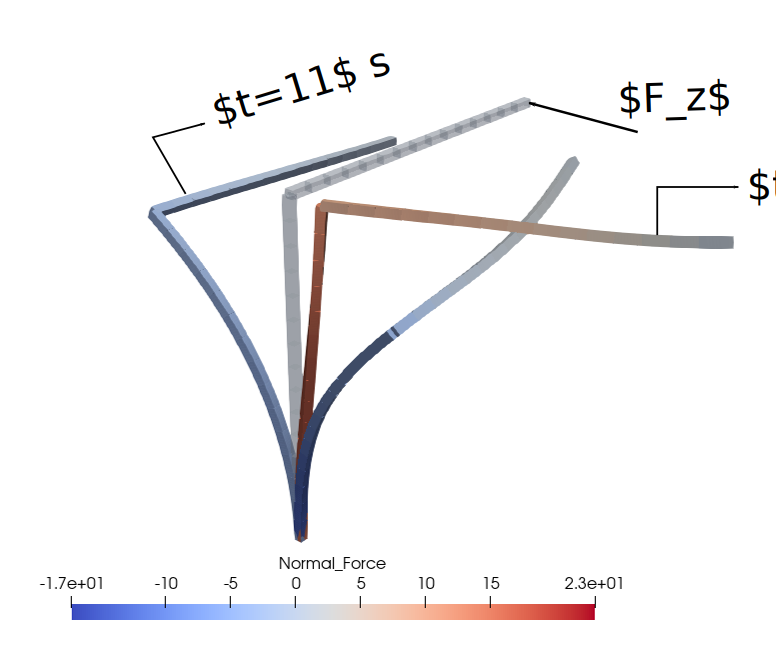
\includegraphics[width=120mm]{./imagenes/ResultadosNumericos/TransmissionTormenta/Deformadas.png}
	\caption{Estructura indeformada y deformada para $t=400$ s.}
	\label{fig:RN:Transmission:Deformadas}
\end{figure} 
 		% Se carga el capítulo 05
  \chapter{Conclusiones}\label{Cap:Conlcusiones}
\linenumbers

El presente capítulo puede separarse en tres secciones que se relacionan con diferentes aristas o perspectivas del trabajo llevado a cabo. En primera instancia, se detallan las consideraciones finales y de síntesis, desde un punto de vista técnico sobre los resultados obtenidos. Posteriormente, se narran los aspectos del desarrollo académico de esta tesis como trabajo culmine dentro de una etapa formativa fundamental para quien escribe. Luego de esto, se realizan recomendaciones y posibles trabajos a futuro para finalizar con una reflexión sobre las limitaciones críticas de este trabajo y el método científico en general. 

\section{Conclusiones técnicas}

\subsection{Sobre el fenómeno}
Según la bibliografía consultada hay vasta evidencia de que el fenómeno de tormentas convectivas ha afectado severamente la calidad e integridad de vida a lo largo y ancho del globo terráqueo. En particular, debido condiciones climáticas singulares de la región, y el progresivo calentamiento global, han intensificado los daño devastadores en los sistemas de trasmisión y distribución eléctrica nacionales. Induciendo inevitablemente en costos millonarios de reparación sobre las instalaciones y mas las perdidas de ganancias durante interrupción del suministro. Además, estos eventos extremos se manifiestan en corrientes descendentes o tornados extra-tropicales que han puesto en peligro la salud y condiciones de vida de las personas. 

A partir de las bibliografías consultadas y los resultados del  ejemplo \ref{Sec:RN:TransmissionSystem}posible teorizar que la mayoría de las incidencias ocurridas en las líneas Palmar-Montevideo de 500kV pueden deberse al pasaje de tormentas severas sobre la zona. Estas tormentas producen corrientes descendentes que ejercen cargas desmesuradas sobre el conductor, en el orden de minutos, imponiendo ángulos de balanceo excesivos que acercarían los conductores a las torres a una distancia tal que inminentes descarga a tierra pueden sacar del serivcio a la linea. Además según los estudios, el diseño de sistemas de trasmisión considerando flujos tipo capa límite atmosférica poliandria estar subdimensionando ya que los periodos de retorno para velocidades de hasta 100 km/h es menor para corrientes descendentes respecto de vientos capa límite atmosférica. 

Dada la problemática esta investigación la atacó  generando herramientas de simulación computacional, capaces de emular los desmedidos desplazamientos y esfuerzos que estos eventos producen sobre los sistemas de trasmisión eléctrica de alta tensión. Para esto, inicialmente se consulto el estado del arte desde un foco de ingeniería del viento y estructural. Se analizaron bibliografías en materia de simulaciones numéricas aplicadas a conducentes eléctricos, con abordajes semi analíticos y computacionales. También, se estudiaron trabajos nacionales e internacionales, desde un punto de vista cualitativo y experimental de corrientes descendentes y sus posibles perjucios  en lineas de trasmisión eléctrica.  Asimismo, el autor se interiorizó y eligió la formulación corrotacional de vigas 3D. Una vez ahondado en la temática, se implementó y validó un modelo corrotacional consistente robusto y eficaz capaz de captar y reproducir desplazamientos de gran amplitud con numero reducido de elementos.


\subsection{Sobre los resultados}

Esta formulación se valido con el ejemplo \ref{Sec:RN:RightAngle} benchmark del folclore corrotacional presentado por \cite{simo1988dynamics}. Este es cargado con una fuerza abrupta y de severa magnitud, respecot al  rigidez de la estructura alcanzando un valor de 50 $N$ en apenas 2 segundos de simulación, tal y como se muestra en la Figura \ref{fig:RN:RA:Force}. Esta fuerza pose una esencia análoga al fenómeno de tormentas convectivas per se. Esta fuerza aumenta estrepitosamente en un corto lapso de tiempo, por ende la capacidad del modelo de reproducir este tipo de impactos es fundamental para poder emular el fenómeno central de este trabajo en simulaciones de sistemas eléctricos.

 En la Figura \ref{fig:RN:RA:Dispz} se observan amplitudes que alcanzan las 8 metros cuando la estructura mide 10. Esto evidencia, la fuerte presencia de grandes desplazamientos y rotaciones. Asimismo, en la dirección $z$, se puede observar el carácter no conservativo de la formulación corrotacional, ya que los valles y crestas de las respuesta prestan una tendencia decreciente con el tiempo. En relación con los desplazamientos en el sentido de $y$ del nodo A, presentados en la Figura \ref{fig:RN:RA:DispyA}, se observa el singo negativo de este, concordando con lo esperado intuitivamente según el sentido de la fuerza aplicada. Por último, el resultado mas importante de este ejemplo se destila al cotejar las respuestas del as Figuras \ref{fig:RN:RA:DispyA}, \ref{fig:RN:RA:DispzA} y \ref{fig:RN:RA:DispzB} con lo publicado por le articulo de referencia \citep{Le2014}. Al comparar estas figuras se concluye que el modelo implementado es capaz de representar cabalmente movimientos de gran amplitud, con apenas 10 elementos por miembro y unas paso temporal de 0.25 $s$. Esto permitíó validar la formulación para este ejemplo y aplicarla a dominios mas complejos específicamente con el foco en el modelado de conductores eléctricos. 







% Esta formulación se aplico específicamente a conductores de alta tensión sometidos perfiles de viento extraídos de artículos recientes aplicados a tormentas convectivas. Las respuestas del sistema evidencian el balanceo excesivo del conductor \ref{fig:DeformadasEqual}, ante este tipo de solicitaciones, los códigos generados pueden gestar una herramienta de análisis complementario para el diseño de sistemas de trasmisión eléctrica. Al vincular 		\ref{fig:CableDispY} y \ref{fig:CableFuerzaZ} se evidencian la idéntica forma que desarrollan ambo perfiles colmando las expectativas sobre dicha salida.


\section{Conclusiones de formación}
El desarrollo de este trabajo constituyó una instancia de formación fundamental y enriquecedora para el autor enmarcada dentro del programa de Magister en Ingeniería Estructural. Este documento es la síntesis y aplicación de un conjunto de conocimientos profundizados durante la actividad programada, aplicada al modelado numérico de estructuras. Desde la óptica del autor, la creación de herramientas endogenas con foco en atacar problemáticas a nivel nacional constituye un pilar fundamental en el desarrollo autónomo y original de la ingeniería uruguaya. Este trabajo es una muestra de la convicción y determinación, que el conocimiento académico, debe desarollarse de forma transparente, comunitaria y democrática. Es por esto, que todos los códigos utilizados en esta investigación se implementaron en el software libre \href{https://github.com/ONSAS/ONSAS/}{ONSAS}. Esto abre la posibilidad a cualquier tercero ya sea una organización o persona de estudiar, modificar y difundir los códigos creados como también aplicarlos a sus propias necesidades. 

\section{Limitaciones }




\section{Trabajos a futuro}



%Con respecto a la norma se esclarecieron las metodologías propuestas para el diseño de lineas de trasmisión,  se corroboraron los valores supuestos por la norma con diferentes referencias, algunas expuestas en el curso, y otras investigadas. Se destaca como debilidad que para el diseño que esta no considera eventos de vientos no sinópticos, estos pueden vulnerar al sistema, como se observaron en distintas bibliografías, solo se consideran viento tipo capa límite atmosférica. 


%Para el análisis del  problema en particular, se creó una librería que contiene un conjunto de códigos que, mediante el método de elementos finitos e iteraciones de Newton-Raphson, resuelve dicho problema para diversas condiciones de borde.  Se concluye que este es capaz de reproducir de forma adecuada el balanceo del cable en contraste con \cite{Stengel2017}. Las desviaciones entre los 230 y 500 segundos pueden estar asociadas a errores durante la toma de datos del perfil de velocidades y/o términos no inerciales de magnitud apreciable, en este período no sería válido aplicar un modelo estático como se realiza en \cite{Stengel2017}. El software permite obtener los modos normales, y plotear sus modos asociados sobre la configuración indeformada, además se generaron vídeos para cada uno de estos modos los cuales se adjuntan en la carpeta del código. Los modos de vibración constituyen un importante resultado a contrastar con las frecuencias predominantes en el flujo, para el ejemplo se encuentran alejadas en al menos un orden de magnitud, sin embrago otras geometrías podrían producir resonancias dinámicas, aumentándose significativamente la amplitud de oscilación. 

%Como trabajo a futuro se debería incluir un modelo de vigas a flexión,  dinámico y no lineal que represente completamente el cambio de rigidez e inercia a lo largo de la trayectoria del conductor. En relación a esto un modelo correccional presentado en las referencias \cite{Le2014} y \cite{Le2011} se ajusta a las necesidades. 		% Se carga el capítulo 06
%
%  % Seguir copiando la linea de arriba para agregar más capítulos.
%  
  \backmatter % Comando que generalos apéndices, anexos y bibliografía. NO COMENTAR
%  
%
  \printbibliography[heading=bibintoc]		% Se imprimen las referencias bibliográficas
  \bibend % NO comentar
%  % 
 \glosario 		         % Glosario, NO comentar
%  %
  \apenarabicnumbering
  \apenmatter				 % Apéndices, NO comentar
  \chapter{Códigos implementados}\label{Ape1}

En este apéndice se presenta el código de la principal función implementada en (\href{https://github.com/ONSAS/ONSAS.m/}{ONSAS}) donde el autor incorporó los términos dinámicos de fuerzas inerciales y matrices tangentes estudiadas.
%\lstset{language=Matlab,%
%	%basicstyle=\color{red},
%	breaklines=true,%
%	morekeywords={matlab2tikz},
%	keywordstyle=\color{blue},%
%	morekeywords=[2]{1}, keywordstyle=[2]{\color{black}},
%	identifierstyle=\color{black},%
%	stringstyle=\color{mylilas},
%	commentstyle=\color{mygreen},%
%	showstringspaces=false,%without this there will be a symbol in the places where there is a space
%	numbers=left,%
%	numberstyle={\tiny \color{black}},% size of the numbers
%	numbersep=5pt, % this defines how far the numbers are from the text
%	emph=[1]{for,end,break},emphstyle=[1]\color{red}, %some words to emphasise
%	%emph=[2]{word1,word2}, emphstyle=[2]{style},    
%}

%\lstinputlisting{elementBeamForces.m}
\lstinputlisting[language=Octave]{elementBeamForces.m}
  \chapter{Revisión de normativa internacional}\label{Ape2}

En esta sección se exponen las secciones destacadas de la norma internacional \cite{IEC60826}, explicitándose las hipótesis fundamentales y el procedimiento para el diseño de elementos de transmisión eléctrica. También se corroboró efectivamente que la norma estudiada considera exclusivamente vientos tipo CLA.

\section{Campo de aplicación}
El campo de aplicación de la norma está sujeto a los siguientes requerimientos sobre el conductor y el terreno:

\begin{itemize}
	\item La longitud de vano debe pertenecer al intervalo ($200$ m, $800$ m). Para longitudes fuera de ese rango deben analizarse coeficientes de racha diferentes a los presentados, sin embargo para vanos más largos a $800$ m el análisis de la norma resulta sobrestimado.
	\item Altura de soportes menores a $60$ m ya que los soportes de una altura mayor podrían inducir factores de amplificación dinámicos en la respuesta.
	\item La línea debe estar a una altura menor a los $1300$ msnm.
	\item Los terrenos no pueden tener características topográficas singulares cuyo tamaño y forma puedan afectar las consideraciones respecto al flujo.
\end{itemize}

\section{Velocidad de referencia y rugosidad del terreno}
Se establecen diferentes tipos de terrenos según las condiciones topográficas del mismo, esto afecta la forma del flujo considerado para el diseño. Para un perfil tipo ley potencial, terrenos más rugosos acentúan el gradiente de la velocidad en la altura de referencia $z=0$,  aumentando la intensidad de turbulencia e incrementando el valor donde el perfil alcanza la atmósfera libre $Z_G$.

\begin{table}[h] 
	\begin{footnotesize} 
		\begin{center} 
			\begin{tabular}{|c||c|}
				\hline
				\textbf{Categoría de terrenos}& \textbf{Características del terreno}  \\\hline
				A & Largos y estrechos viento de ultramar,  \\
				& área costera llana, llanura desértica.    \\ \hline
				B & Campo abierto con escasa densidad de obstáculos. \\
				& áreas cultivadas con pocos árboles y edificios     \\ \hline
				C &  Terreno con numerosos obstáculos pequeños de baja altura \\
				& (matorrales, árboles y edificios)  \\ \hline
				D & Áreas sub-urbanas con pequeños arboles     \\ \hline
			\end{tabular}
		\end{center} 
		\caption{Categorización de terrenos Tablas A.8 IEC 60826}
	\end{footnotesize} 
	\label{TablaTerrenos} 
\end{table}

Considerando un flujo medio plano tipo CLA, una atmósfera neutra y diferentes constantes de terreno $\alpha$, entonces la velocidad media en altura $v(z)$ se puede calcular de la siguiente manera:

\begin{equation}\label{LeyPotencial}
	V(z)=V_{G}\left(\frac{z}{z_{G}}\right)^\alpha
\end{equation}

Medidas de velocidad utilizando artefactos, como anemómetros o sensores de ultra sonido, permiten obtener para un determinado periodo de adquisición de datos, valores de velocidad media e intensidad de turbulencia. Es por esto, que es clave relacionar la velocidad a diferentes alturas y para cambios de terreno a lo largo del sentido del flujo. Definiendo $V_{ref}$ como la velocidad media del viento a una altura de $z=10$ m para un tipo de terreno categoría B y llamando a dos puntos a diferentes alturas 1 y 2, es posible relacionar su velocidad media según:

\begin{equation}\label{RelacionPotencial}
	V(z)=V_{ref1}\left(\frac{z_{G1}}{z_{ref}}\right)^{\alpha_1}\left(\frac{z}{z_{G2}}\right)^{\alpha_2}.
\end{equation}

En la Ecuación \eqref{RelacionPotencial} se introduce un factor $K_R$ el cual permite obtener la relación entre las velocidades de referencia para distintos terrenos $V_{rX}=K_RV_{rB}$. En la Tabla \ref{Tab:laValoresTerrenos} las diferentes alturas de rugosidad media de obstáculos $z_0$.


\begin{table}[h] 
	\begin{footnotesize} 
		\begin{center} 
			\begin{tabular}{ |p{3cm}|p{2cm}|p{2cm}|p{2cm}|p{2cm}|} \hline
				\multirow{2}{*}{\textbf{Factor}}  & \multicolumn{4}{|c|}{ \textbf{Categoría de terreno} }  \\ 
				& \textbf{A}& \textbf{B} &\textbf{C}&\textbf{D}\\
				\hline
				$z_0(m)$   & 0.01    &0.05&  0.30 & 1.00\\ \hline
				$\alpha$& 0.1 a 0.12  & 0.16 & 0.22 &0.28\\ \hline
				$K_R$ & 1.08 &1.00 &0.85&  0.67\\ \hline
			\end{tabular}
		\end{center} 
		\caption{Tabla de factores para terrenos Tabla A.8 IEC 60826.}
		\label{Tab:laValoresTerrenos} 
	\end{footnotesize} 
\end{table}

En los datos presentados en la Tabla \ref{Tab:laValoresTerrenos}, los valores de $\alpha$ se asemejan con lo presentado por \cite{Davenport1960}, para la categoría A y B el número de $\alpha$ considerado por la norma es menor, esto se fundamente en que valores menores de $\alpha$, es decir terrenos menos rugosos, inducen una velocidad mayor para la misma cota. En el caso de la categoría C y D el valor es exactamente idéntico a lo propuesto en \citep{Davenport1960} . De igual forma el término $z_0$ se condice con la Tabla publicada en \citep{Oke2000}.

Desglosando el factor $K_R$ para dos puntos de referencia, colocados a una cota de $z_{ref1}=z_{ref2}=10$ m en función de la Ecuación \eqref{RelacionPotencial} y combinándola con la definición de $K_r$ se obtiene la siguiente expresión: 

\begin{equation}\label{ValorKR}
	V_{ref2}(10m)=V_{ref1}\left(\frac{z_{G1}}{z_{ref1}}\right)^{\alpha_1}\left(\frac{z_{ref2}}{z_{G2}}\right)^{\alpha_2}\rightarrow K_r=\left(\frac{z_{G1}}{z_{ref1}}\right)^{\alpha_1}\left(\frac{z_{ref2}}{z_{G2}}\right)^{\alpha_2}
\end{equation}

Sustituyendo la Ecuación \ref{ValorKR}  y considerando los valores de $Z_G$ según la referencia \citep{Oke2000} se expresan los resultados obtenidos: l

\begin{table}[h] 
	\begin{footnotesize} 
		\begin{center} 
			\begin{tabular}{ |p{3cm}|p{2cm}|p{2cm}|p{2cm}|p{2cm}|} \hline
				\multirow{2}{*}{\textbf{Factor}}  & \multicolumn{4}{|c|}{ \textbf{Categoría de terreno} }  \\ 
				& \textbf{A}& \textbf{B} &\textbf{C}&\textbf{D}\\
				\hline
				$z_G(m)$   & 250     &305&  365 &410\\ \hline
				$\alpha$& 0.12  & 0.15 & 0.22 &0.28\\ \hline
				$K_R$ & 1.13 &1.00 &0.77&  0.61\\ \hline
			\end{tabular}
		\end{center} 
		\caption{Tabla de factores para terrenos según referencia \cite{Davenport1960} }
	\end{footnotesize} 
	\label{TablaValoresTerrenos} 
\end{table}
Estos coinciden con un error menor al $8\%$ con los estipulados por la norma en la Tabla \ref{Tab:laValoresTerrenos}. Lo que comprueba que efectivamente para estimar las velocidades se considera un viento tipo CLA. 

%\section{Acción del viento sobre los elementos}
%
%El valor significativo del problema es la fuerza por unidad de área (Pa) se denota con la letra $a$ además se define, al igual que lo visto en el curso en la sección 2.1 del repartido "Bluff-Body aero dynamics"  $q0$, el coeficiente de presión dinámica de referencia $(N/m^3)$. Para elementos conductores, cadenas y gran cantidad de elementos de soportes se calcula:
%
%\begin{eqnarray} \label{CoficienteDin1}  
%	a&=&q_0C_xG \\\label{CoefDin2}
%	q_0&=&\frac{1}{2}\rho_{ref} \tau \left ( K_rV_{rB}\right )^{2}
%\end{eqnarray}
%
%En las Ecuaciones \ref{CoficienteDin1} y \ref{CoefDin2} $\rho$ es la densidad del aire en $kg/m^{3}$ y se toma en $1.225 \vspace{0.1cm} kg/m^{3}$ para una temperatura de $15^{\circ}C$  y una presión atmosférica de $101.3 \vspace{0.1cm} kPa$. La constante $\tau$ es un factor que permite corregir las variaciones de densidad del fluido con la presión medida en altura y la temperatura a la que operará el sistema. Los valores de densidad se corroboraron con la referencia \cite{cengel2007termodinamica}, como también el factor de corrección $\tau=\frac{\rho_{P,T}}{\rho_{ref}}$.
%
%El parámetro $C_x$ es el coeficiente de drag dependiendo de la figura transversal al flujo, se desprecian por las grandes longitudes de vanos las condiciones de borde no homogéneas del flujo en los extremos. Por último el factor restante $G$ toma en consideración la altura y el tipo de terreno, el incremento en la velocidad de acuerdo a ráfagas de viento y la respuesta dinámica, para elementos de cable debe separarse en $G_L$ y $G_c$. Estos últimos factores se vincularán  en la siguiente sección con los conocimientos presentados en el curso. 
%
%
%
%
%\section{Elementos de cable}\label{ElemCableNorma}
%Los efectos dinámicos que afectan a los conductores específicamente se asocian: al arrastre producido por el viento y la tensión mecánica incrementada durante la instalación. Considerando la hipótesis de baja turbulencia, la fuerza media en Newton de arrastre ($A_c$) sobre un elemento de largo $L$ y diámetro $d$, formando un ángulo de balanceo $\Omega$ es dada por la expresión:
%
%\begin{equation} \label{EqnFuerzaCable}
%	A_c=q_0C_{xc}G_cG_L d L \sin(\Omega) ^{2}
%\end{equation}
%
%En la Ecuación \ref{EqnFuerzaCable} el factor de presión de referencia ($q_0$) se calcula según la Ecuación  \ref{CoficienteDin1}. El valor de $C_{xc}$ es el coeficiente de drag del conductor, su utiliza a menos de obtenerse datos experimentales, un valor unitario para conductores y velocidades de viento estándar. Esto se corresponde con lo presentado en el curso en la figura 19 de \citep{Duranona2018} a velocidades equivalentes de $5m/s$ para un conductor usual de alta tensión. Según \cite{Son2016} se hallan valores medios del coeficiente de drag para Reynolds de aproximadamente igual $350$ $C_{xc}$ y resulta ser 1. Es por esto que considerar un valor unitario para valores los valores Reynolds de trabajo induciendo una fuerza de mayor magnitud sobre el cable, lo cual es conservador. 
%
%Existe un efecto en la dirección perpendicular al flujo  llamado "Aeolian". En dicha dirección se generan desprendimientos de vórtices asociados con la frecuencia de Strouhal $f_s=0.0925\frac{v_m}{d_c}$, cuando estos vórtices se acercan a la frecuencias naturales del cable podrían producirse resonancias, magnificándose las amplitudes del movimiento. Según \cite{Belloli2006} estos efectos deben ser considerados para velocidades medias de viento menores $6\frac{m}{s}$ , para el estudio de \gls{TC} las velocidades alcanzan valores de hasta $30\frac{m}{s}$ estando el efecto antes mencionado fuera de rango. 
%
%
%El coeficiente $G_c$ es el factor de viento combinado, el cual se halla con la Figura 3 de la Sección 6.2.6.1,  este depende de la altura y el tipo de terreno.
%Según de lo visto en el curso este debe contener el factor de ráfaga el cual relaciona la presión media con la máxima puntual. Por último $G_l$ es el factor de separación según el largo de vano, este tiene en cuenta la distribución de presiones para distintos largos de vano, para vanos largos la presión máxima se da simultáneamente en pocos puntos por tanto decrece, tal como se ve en la Figura 4 de la Sección 6.2.6.1 y se corresponde con lo visto en el curso para el valor de B.
%
%
%
%Para cadenas aisladoras múltiples que transporten  más de un cable, estos deben tratarse por separado, las solicitaciones totales sobre los soportes deben considerarse la suma de cada una de las partes. La altura considerada para el cálculo de los factores debe ser el centro de gravedad de los conductores cuando este se encuentra a 2/3 de la deflexión máxima. También puede considerarse la altura como la cota del punto de anclaje entre la cadena y el cable, esto inducirá velocidades mayores y por tanto el diseño estará sobredimensionado. 
%
%
%\subsubsection{Cargas del viento sobre la cadena aisladora}
%Las cargas actuando en el elemento aislador cerámico se originan sobre el área proyectada de la cadena en el sentido del flujo, la cual se nombra $A_c$. Esta carga se corresponde a la suma de las cargas debido al campo de presiones sobre el cable y la fuerza distribuida directamente sobre la cadena aisladora. La carga aplicada sobre el soporte $A_l$ en N se expresa: 
%\begin{equation} \label{FuerzaSoprotes}
%	A_l=q_0C_{xl}G_tS_i
%\end{equation}
%En la Ecuación \ref{FuerzaSoprotes} el factor $q_0$ es la presión dinámica de referencia calculada según \ref{CoficienteDin1}, $C_{xl}$ se asocia con el Coeficiente de Drag y se suele considerar $1,2$, valor mayor que para el cilindro. Se aclara que en general el peso relativo de la fuerza sobre los soportes debido a las cadenas aisladoras es significativamente menor respecto a las cargas del viento ejercidas sobre el conductor. 
%
%
%
%El termino $G_t$ es el factor de viento correlativo que se corresponde con la Figura 5 de la norma de la sección 6.2.6.3, este se ve afectado por el tipo de terreno y la altura del centro del gravedad de la cadena, este al igual que en la Sección \ref{ElemCableNorma} el combinado de los factores vistos en el curso. Esta presión es multiplicada por el valor $S_i$ del área de la cadena proyectada horizontalmente en un plano paralelo al eje de la torre en $m^2$.

  \chapter{Conclusiones del autor}\label{Ape3}
El desarrollo de este trabajo constituyó una instancia de formación fundamental y enriquecedora enmarcada dentro del programa de Maestría en Ingeniería Estructural. Este documento es la síntesis y aplicación de un conjunto de conocimientos profundizados durante la actividad programada, aplicada al modelado numérico de estructuras. La creación de herramientas endógenas con foco en atacar problemáticas a nivel nacional constituye un pilar fundamental en el desarrollo autónomo y original de la ingeniería uruguaya. Este trabajo es una muestra de la convicción y determinación, que el conocimiento académico, debe desarrollarse de forma transparente, comunitaria y democrática. Es por esto, que todos los códigos utilizados en esta investigación se implementaron en la herramienta de software libre \href{https://github.com/ONSAS/ONSAS.m/}{ONSAS}. Esto abre la posibilidad a cualquier tercero, ya sea una organización o persona, de estudiar, modificar y difundir los códigos creados como también aplicarlos a sus propias necesidades. 
\subsection{Reflexión personal}
Antes que nada, es necesario realizar una arqueología de las palabras sujeto y fenómeno en castellano. Sujeto en latín \emph{sub}-{iectum} significa lo que está debajo, según una interpretación posmoderna. Desde esta perspectiva, es el sujeto el sustrato de cualquier ente, que lo dota de sustancia, colores, palabras y formas. Por otra parte, fenómeno tiene una raíz etimológica en la palabra \emph{phainomenon} al igual que la palabra fantasía. Esto alude a lo que se muestra, lo que se deja ver, lo que brilla. Ahora bien, en el acto de percibir cognitivamente existe una dirección previa (inconsciente o consciente) de apuntar el foco hacia algo, entonces ¿Quién y cómo se dirige ese foco?

Toda disciplina e investigación debería conocer sus propias fugas, fronteras y puntos ciegos. De lo contrario, cualquier pretensión hermética podría ser un síntoma de arrogancia y altanería.  A lo largo de este trabajo, he canonizado una redacción en tercera persona, como si existiese una determinada imparcialidad y transparencia en dicho escritor. O quizás una búsqueda con necedad de la verdad absoluta. Este sujeto, apuntado y enfocado en los párrafos siguientes, merece ensimismarse y cuestionarse a sí mismo, según el proverbio en templo de Apolo del Oráculo de Delfos, \emph{gnóthi sautón} o en castellano \emph{Conócete a ti mismo}.

Durante el transcurso de este trabajó me surgieron las siguientes inquietudes ¿Es la realidad un conjunto de fenómenos externos o es siempre un acto de interpretación inmanente al sujeto? Además, ¿Ese sujeto accede la realidad (el objeto) a través de la razón para conocer y explicarla, o simplemente la experiencia es quien valida ese conjunto de fenómenos? A partir de esta pregunta, emana una interrogante natural, ¿Es posible entonces, desligar al sujeto del objeto, o más bien este ente (ex-siste) en el mundo, y está siempre arrojado, lanzado y en relación con el? Y de ser así, ¿No se encuentra entonces \textbf{ya} sugestionado por el paradigma actual, su cultura nativa y sus experiencias personales cuando describe?

Esas preguntas han sido abordadas por eminencias de la filosofía y la ciencia, desde la modernidad hasta hoy. Por un lado, el realismo científico concibe que es posible constatar la realidad a través de la experiencia o a través del pensamiento. Para Descartes ese sujeto duda, piensa y por tanto \textbf{ya} en ese acto analítico, existe (\emph{Cogito ergo sum}) \cite{descartes2004discurso}, ósea el ente en tanto ente. El padre del racionalismo nos plantea que es el yo del sujeto, quien a través de la duda metódica puede acceder la verdad. Contrapuesto a este, el empirismo valida cualquier conocimiento sólo por la experiencia. Esta se define por lo que es captado por nuestros sentidos, es decir que la experiencia es sensorial. Estas dos posturas, la del racionalismo de Descartes y la del empirismo de Hume, pueden ser pensadas como una forma de abordaje a la relación realidad - conocimiento. Para Descartes: conozco en tanto analizo y pienso, y los objetos existen cuando yo realizo la abstracción. Para el empirismo: conozco en la medida en que incorporo la realidad ``objetiva", la de los objetos que puedo percibir a través de los sentidos. 

A mediados del sg XIX nació un pensador disruptivo que viró absolutamente a la cuestión. Frederick Niezstche plantea en su libro Voluntad de Poder \cite{nietzsche2018voluntad} `` El pensar no es para nosotros un medio para ``conocer" sino para designar el acontecer, para ordenarlo, para volverlo manejable para nuestro uso: así pensamos hoy acerca del pensar: mañana quizá de otro modo ". Esta frase alude, desde mi voz de hoy, a un nihilismo que niega la posibilidad de conocer algo absoluto verdadero pues no es más que un desarrollo pragmático de poder. Es una cuestión de voluntad de voluntad, un dispositivo ordenatorio de la realidad según categorías y características en nuestro acto de querer/poder conocer. Antípoda a esta teoría nihilista aparece el relativismo. Este se estriba en el principio de incertidumbre Heisenberg, si existe ese conocimiento, es entonces indisoluble de cierta estructura. Thomas Khun en su libro \emph{La estructuras de las revoluciones científicas} \cite{kuhn2019estructura} plantea que el método científico revoluciona, cuando se produce un cambio de paradigma, no a partir de la observación de nuevos hechos o fenómenos. Junto con otros destacados sociólogos, acuñan la idea del concepto de ``cargado de teoría", un cierto conjunto de preconceptos anteriores a la observación, descripción y desarrollo de la cualquier investigación, que llevarán al científico demostrar lo que realmente quiere demostrar... de nuevo demostración de poder.

¿Como se demuestran los resultados de esta investigación?, construyendo un conjunto de artefactos experimentales/computacionales que constatan una supuesta realidad casi como un espejo, por correspondencia. En ese proceso de creación o utilización de instrumentos como ser: un programa, un anemómetro o un código computacional existe una omnipresente intervención humana. ¿Vale entonces seguir redactando en tercera persona desde un objetivismo positivista heredado de hace dos siglos? ¿Es coherente no ser impersonal la descripción de un resultado, cuando \textbf{ya} todo el dispositivo ordenatorio que subyace es una construcción humana? ¿Debemos seguir defendiendo un cadáver \textbf{ya} asesinado por las ciencias humanas, desde un \textbf{sujeto que no es más que un efecto} cultural, histórico y económico?. ¡Por una ciencia que tenga con-ciencia de sus puntos ciegos, Por una ciencia con con-ciencia de que la verdad absoluta ha muerto, Por una ciencia construida por personas en primera persona!  
%  % Seguir copiando la linea de arriba para agregar más apéndices.
%  %
%  \anexarabicnumbering
%  \anexmatter				 % Anexos, NO comentar
%  \chapter{}\label{Ane1}
Se acoplan al tesis una revisión bibliográfica realizada en el marco del curso Elementos de Aerodinámica y Aeroelasticidad de Estructuras en su edición 2019 sobre la norma \cite{IEC60826}.
\section{Norma IEC 60826} \label{NormaIEC}
En este apartado se exponen las secciones destacadas de la norma internacional IEC 60826: \cite{IEC60826}, explicitándose las hipótesis fundamentales y  formulaciones para el desarrollo de condiciones de diseño. 

\subsubsection{Campo de aplicación}
En primera medida esta aplica para geometrías del conductor y terreno con las siguientes condiciones:

\begin{itemize}
	\item La longitud de vano debe pertenecer al intervalo (200\vspace{0.1cm}m, 800\vspace{0.1cm}m). Para longitudes fuera de ese rango deben analizarse coeficientes de racha diferentes a los presentados, sin embargo para vanos más largos a 800m el análisis de la norma resulta sobrestimado.
	\item Altura de soportes menores a 60 \vspace{0.1cm}m. Soportes de mayor altura podrían inducir factores de amplificación dinámicos de la respuesta.
	\item Altitud del área transversal de la línea no sobrepase los 1300\vspace{0.1cm}m sobre el nivel de altura medio topográfica del terreno circundante.
	\item Terrenos  sin características topográficas singulares cuyo tamaño y forma puedan afectar las consideraciones del flujo. Se aclara que esta norma \ textit{no permite dimensionar para efectos de vientos extremos como tornados, encause de vientos entre montañas y terrenos de alta pendiente. }
\end{itemize}

\subsubsection{Velocidad de referencia y rugosidad del terreno}
Como primera instancia se establecen diferentes tipos de terrenos según las condiciones topográficas del mismo, esto afecta la forma del flujo considerado para el diseño. Para un perfil tipo ley potencial, terrenos más rugosos acentúan el gradiente de la velocidad en altura para $z=0$,  aumentan la intensidad de turbulencia e incrementan el $Z_G$ (valor donde el perfil alcanza las condiciones de atmósfera libre). 


\begin{table}[h] 
	\begin{footnotesize} 
		\begin{center} 
			\begin{tabular}{|c||c|}
				\hline
				\textbf{Categoría de terrenos}& \textbf{Características del terreno}  \\\hline
				A & Largos y estrechos viento de ultramar,  \\
				& área costera llana, llanura desértica.    \\ \hline
				B & Campo abierto con escasa densidad de obstáculos. \\
				& áreas cultivadas con pocos árboles y edificios     \\ \hline
				C &  Terreno con numerosos obstáculos pequeños de baja altura \\
				& (matorrales, árboles y edificios)  \\ \hline
				D & Áreas sub-urbanas con pequeños arboles     \\ \hline
			\end{tabular}
		\end{center} 
		\caption{Categorización de terrenos Tablas A.8 IEC 60826}
	\end{footnotesize} 
	\label{TablaTerrenos} 
\end{table}




Considerando un flujo medio plano tipo capa límite potencial, que se desarrolla en una atmósfera neutra, la velocidad media $v(z)$ en función de la altura para diferentes constantes de terreno $\alpha$ puede calcularse de la siguiente manera:

\begin{equation}\label{LeyPotencial}
	V(z)=V_{G}\left(\frac{z}{z_{G}}\right)^\alpha
\end{equation}

Medidas de la velocidad a través de equipos como pueden ser anemómetros o sensores de ultra sonido permiten obtener, para determinado periodo de adquisición de datos, valores de velocidad media e intensidad de turbulencia entre otras. Es por esto que es clave relacionar la velocidad a diferentes alturas y para cambios de terreno a lo largo del sentido del flujo, nombrando dos puntos 1 y 2 podemos relacionar la velocidad media entre estos operando con la Ecuación \eqref{LeyPotencial}.

\begin{equation}\label{RelacionPotencial}
	V(z)=V_{ref1}\left(\frac{z_{G1}}{z_{ref}}\right)^{\alpha_1}\left(\frac{z}{z_{G2}}\right)^{\alpha_2}
\end{equation}

En la Ecuación \ref{ elacionPotencial} anterior la velocidad de referencia $V_{ref}$ es definida, en general como la velocidad media del viento a una altura de $z=10\vspace{.1cm}m$ para un tipo de terreno categoría B. En la norma se presenta la siguiente tabla para calcular las variaciones de velocidad $V_{ref}$, se introduce un factor $K_R$ el cual permite obtener la relación entre las velocidades de referencia para distintos terrenos $V_{rX}=K_RV_{rB}$. Se presentan las diferentes alturas de rugosidad media de obstáculos $z_0$.


\begin{table}[h] 
	\begin{footnotesize} 
		\begin{center} 
			\begin{tabular}{ |p{3cm}|p{2cm}|p{2cm}|p{2cm}|p{2cm}|} \hline
				\multirow{2}{*}{\textbf{Factor}}  & \multicolumn{4}{|c|}{ \textbf{Categoría de terreno} }  \\ 
				& \textbf{A}& \textbf{B} &\textbf{C}&\textbf{D}\\
				\hline
				$z_0(m)$   & 0.01    &0.05&  0.30 & 1.00\\ \hline
				$\alpha$& 0.1 a 0.12  & 0.16 & 0.22 &0.28\\ \hline
				$K_R$ & 1.08 &1.00 &0.85&  0.67\\ \hline
			\end{tabular}
		\end{center} 
		\caption{Tabla de factores para terrenos Tabla A.8 IEC 60826.}
	\end{footnotesize} 
	\label{TablaValoresTerrenos} 
\end{table}

Los datos presentados en la Tabla \eqref{TablaValoresTerrenos} se corresponden con los conocimientos dictados en el curso, en primera parte los valores de $\alpha$ se asemejan con lo presentado por \cite{Davenport1960}, para la categoría A y B el numero de $\alpha$ considerado por la norma es menor, esto se relaciona con que valores más chicos de $\alpha$, es decir terrenos menos rugosos inducen una velocidad mayor para la misma cota. En el caso de la categoría C y D el valor es exactamente idéntico a \cite{Davenport1960} . El termino $z_0$ se coincide con la tabla publicada en \cite{Oke2000}.

Desglosando el factor $K_R$ para dos puntos de referencia, colocados a una cota de $z_{ref1}=z_{ref2}=10m$ en función de la Ecuación \eqref{RelacionPotencial} y combinándola con la definición de $K_r$ se obtiene la siguiente expresión: 


\begin{equation}\label{ValorKR}
	V_{ref2}(10m)=V_{ref1}\left(\frac{z_{G1}}{z_{ref1}}\right)^{\alpha_1}\left(\frac{z_{ref2}}{z_{G2}}\right)^{\alpha_2}\rightarrow K_r=\left(\frac{z_{G1}}{z_{ref1}}\right)^{\alpha_1}\left(\frac{z_{ref2}}{z_{G2}}\right)^{\alpha_2}
\end{equation}
Utilizando la Ecuación \ref{ValorKR}  y considerando los valores de $Z_G$ según la referencia \cite{Oke2000} se expresan los resultados obtenidos los cuales coinciden con un error menor al $8\%$ con los estipulados por la norma en la Tabla \ref{TablaValoresTerrenos}.

\begin{table}[h] 
	\begin{footnotesize} 
		\begin{center} 
			\begin{tabular}{ |p{3cm}|p{2cm}|p{2cm}|p{2cm}|p{2cm}|} \hline
				\multirow{2}{*}{\textbf{Factor}}  & \multicolumn{4}{|c|}{ \textbf{Categoría de terreno} }  \\ 
				& \textbf{A}& \textbf{B} &\textbf{C}&\textbf{D}\\
				\hline
				$z_G(m)$   & 250     &305&  365 &410\\ \hline
				$\alpha$& 0.12  & 0.15 & 0.22 &0.28\\ \hline
				$K_R$ & 1.13 &1.00 &0.77&  0.61\\ \hline
			\end{tabular}
		\end{center} 
		\caption{Tabla de factores para terrenos según referencia \cite{Davenport1960} }
	\end{footnotesize} 
	\label{TablaValoresTerrenos} 
\end{table}

\subsubsection{Acción del viento sobre los elementos}

El valor significativo del problema es la fuerza por unidad de área (Pa) se denota con la letra $a$ además se define, al igual que lo visto en el curso en la sección 2.1 del repartido "Bluff-Body aero dynamics"  $q0$, el coeficiente de presión dinámica de referencia $(N/m^3)$. Para elementos conductores, cadenas y gran cantidad de elementos de soportes se calcula:

\begin{eqnarray} \label{CoficienteDin1}  
	a&=&q_0C_xG \\\label{CoefDin2}
	q_0&=&\frac{1}{2}\rho_{ref} \tau \left ( K_rV_{rB}\right )^{2}
\end{eqnarray}

En las Ecuaciones \ref{CoficienteDin1} y \ref{CoefDin2} $\rho$ es la densidad del aire en $kg/m^{3}$ y se toma en $1.225 \vspace{0.1cm} kg/m^{3}$ para una temperatura de $15^{\circ}C$  y una presión atmosférica de $101.3 \vspace{0.1cm} kPa$. La constante $\tau$ es un factor que permite corregir las variaciones de densidad del fluido con la presión medida en altura y la temperatura a la que operará el sistema. Los valores de densidad se corroboraron con la referencia \cite{cengel2007termodinamica}, como también el factor de corrección $\tau=\frac{\rho_{P,T}}{\rho_{ref}}$.

El parámetro $C_x$ es el coeficiente de drag dependiendo de la figura transversal al flujo, se desprecian por las grandes longitudes de vanos las condiciones de borde no homogéneas del flujo en los extremos. Por último el factor restante $G$ toma en consideración la altura y el tipo de terreno, el incremento en la velocidad de acuerdo a ráfagas de viento y la respuesta dinámica, para elementos de cable debe separarse en $G_L$ y $G_c$. Estos últimos factores se vincularán  en la siguiente sección con los conocimientos presentados en el curso. 




\subsubsection{Elementos de cable}\label{ElemCableNorma}
Los efectos dinámicos que afectan a los conductores específicamente se asocian: al arrastre producido por el viento y la tensión mecánica incrementada durante la instalación. Considerando la hipótesis de baja turbulencia, la fuerza media en Newton de arrastre ($A_c$) sobre un elemento de largo $L$ y diámetro $d$, formando un ángulo de balanceo $\Omega$ es dada por la expresión:

\begin{equation} \label{EqnFuerzaCable}
	A_c=q_0C_{xc}G_cG_L d L \sin(\Omega) ^{2}
\end{equation}

En la Ecuación \ref{EqnFuerzaCable} el factor de presión de referencia ($q_0$) se calcula según la Ecuación  \ref{CoficienteDin1}. El valor de $C_{xc}$ es el coeficiente de drag del conductor, su utiliza a menos de obtenerse datos experimentales, un valor unitario para conductores y velocidades de viento estándar. Esto se corresponde con lo presentado en el curso en la figura 19 de \cite{Duranona2018} a velocidades equivalentes de $5m/s$ para un conductor usual de alta tensión. Según \cite{Son2016} se hallan valores medios del coeficiente de drag para Reynolds de aproximadamente igual $350$ $C_{xc}$ y resulta ser 1. Es por esto que considerar un valor unitario para valores los valores Reynolds de trabajo induciendo una fuerza de mayor magnitud sobre el cable, lo cual es conservador. 

Existe un efecto en la dirección perpendicular al flujo  llamado "Aeolian". En dicha dirección se generan desprendimientos de vórtices asociados con la frecuencia de Strouhal $f_s=0.0925\frac{v_m}{d_c}$, cuando estos vórtices se acercan a la frecuencias naturales del cable podrían producirse resonancias, magnificándose las amplitudes del movimiento. Según \cite{Belloli2006} estos efectos deben ser considerados para velocidades medias de viento menores $6\frac{m}{s}$ , para el estudio de \gls{TC} las velocidades alcanzan valores de hasta $30\frac{m}{s}$ estando el efecto antes mencionado fuera de rango. 


El coeficiente $G_c$ es el factor de viento combinado, el cual se halla con la Figura 3 de la Sección 6.2.6.1,  este depende de la altura y el tipo de terreno.
Según de lo visto en el curso este debe contener el factor de ráfaga el cual relaciona la presión media con la máxima puntual. Por último $G_l$ es el factor de separación según el largo de vano, este tiene en cuenta la distribución de presiones para distintos largos de vano, para vanos largos la presión máxima se da simultáneamente en pocos puntos por tanto decrece, tal como se ve en la Figura 4 de la Sección 6.2.6.1 y se corresponde con lo visto en el curso para el valor de B.



Para cadenas aisladoras múltiples que transporten  más de un cable, estos deben tratarse por separado, las solicitaciones totales sobre los soportes deben considerarse la suma de cada una de las partes. La altura considerada para el cálculo de los factores debe ser el centro de gravedad de los conductores cuando este se encuentra a 2/3 de la deflexión máxima. También puede considerarse la altura como la cota del punto de anclaje entre la cadena y el cable, esto inducirá velocidades mayores y por tanto el diseño estará sobredimensionado. 


\subsubsection{Cargas del viento sobre la cadena aisladora}
Las cargas actuando en el elemento aislador cerámico se originan sobre el área proyectada de la cadena en el sentido del flujo, la cual se nombra $A_c$. Esta carga se corresponde a la suma de las cargas debido al campo de presiones sobre el cable y la fuerza distribuida directamente sobre la cadena aisladora. La carga aplicada sobre el soporte $A_l$ en N se expresa: 
\begin{equation} \label{FuerzaSoprotes}
	A_l=q_0C_{xl}G_tS_i
\end{equation}
En la Ecuación \ref{FuerzaSoprotes} el factor $q_0$ es la presión dinámica de referencia calculada según \ref{CoficienteDin1}, $C_{xl}$ se asocia con el Coeficiente de Drag y se suele considerar $1,2$, valor mayor que para el cilindro. Se aclara que en general el peso relativo de la fuerza sobre los soportes debido a las cadenas aisladoras es significativamente menor respecto a las cargas del viento ejercidas sobre el conductor. 



El termino $G_t$ es el factor de viento correlativo que se corresponde con la Figura 5 de la norma de la sección 6.2.6.3, este se ve afectado por el tipo de terreno y la altura del centro del gravedad de la cadena, este al igual que en la Sección \ref{ElemCableNorma} el combinado de los factores vistos en el curso. Esta presión es multiplicada por el valor $S_i$ del área de la cadena proyectada horizontalmente en un plano paralelo al eje de la torre en $m^2$.


\subsection{Tensión en el conductor}\label{TensionConductor}
La tensión que debe ser aplicada sobre los conductores se determina a partir del método de deflexión, considérese el caso donde las cadenas aisladoras se encuentra a la misma cota, el conductor tiene un largo L y un peso W por unidad de longitud en N/m, se ilustra un esquema en la siguiente figura:


%
%\begin{figure}[h!]
%	\centering
%	\includegraphics[width=0.6\textwidth]{cuerda.png}
%	\caption{Esquema de un elemento tipo cuerda sobre su propio peso}
%\end{figure}


Considerando el cable como un elemento extensible que no posee rigidez a flexión,  entonces la tensión interna a para cualquier punto de este debe ser tangente a la curva. Sea P un punto cualquiera con coordenadas (x,y) en el cable, tomando equilibrio estático sobre la mitad del conductor y planteado la segunda cardinal o el principio de los trabajos virtuales para un giro arbitrario, desde P, se obtiene la catenaria, y de esta la deflexión máxima en función de la tensión:


\begin{equation}
	Ty=W\frac{x^{2}}{2} \rightarrow \delta= \frac{WL^{2}}{8T}
\end{equation}
%  \chapter{}\label{Ane2}
Se presenta a continuación resultados extraídos de un modelo generado en el marco de la unidad curricular Dinámica de Estructuras. Este consiste en un análisis dinámico 2D y 3D de elementos de biela no lineales con un análisis modal complementario.  


\section{Modelado dinámico de un conductor de alta tensión utilizando elementos de barra}
\subsection{Fundamentos teóricos}

\subsubsection{Ecuación de movimiento}

En este trabajo se utilizará el principio de D’Alambert para establecer las ecuaciones de movimiento de un elemento de barra axial, este es el equivalente dinámico al Principio de los Trabajos Virtuales para el caso estático. A continuación se notará las variables posición, desplazamiento, deformación unitaria y tensión como $(x, u_t ,\epsilon_t,\sigma_t )$  y las derivadas parciales, velocidad y aceleración con $(\dot{u_t} , \ddot{u_t})$.



Dicho lo anterior el principio de D’Alambert afirma que $\forall t$ y $\forall \delta u $ se cumple:
\begin{equation}\label{dalambert}
	\int_{V_t}\sigma_t\delta \varepsilon dV_t=\int_{V_t}\delta u^Tb_{ext,t}dV_t-\int_{V_t}\rho\delta u^T\ddot{u} dV_t
\end{equation}


En la ecuación \eqref{dalambert} $b_{ext,t}$ corresponde a la fuerzas externas por unidad de volumen. El primer termino que aparece restando es el de a las fuerzas inerciales siendo $\rho$ la densidad del material. El segundo corresponde a disipaciones viscosas donde $c>0$. Esta disipación se corresponde con fenómenos de disipación estructural y rozamiento en juntas,  su valor se ajustará de acuerdo con resultados experimentales publicados, no se determinará mediante un resultado teórico. Aplicando una discretización en elementos finitos obtenemos la ecuación de movimiento de la estructura:

\begin{equation}\label{newton}
	M\ddot{u_t}+C\dot{u_t}+K_T(u_t)u_t=f_{ext,t}
\end{equation}

Las cargas externas dinámicas se encuentran asociadas con el vector $f_{ext,t}$. La matriz de rigidez $K(u_t)$ se hallará considerando no linealidad geométrica por ende tiene la siguiente forma:
\begin{equation}
	K_T=K_{T1}+K_{T2}+K_{\sigma} 
\end{equation}
\begin{equation}
	K_{T1}=EA_ol_ob_1^Tb_1
\end{equation}
\begin{equation}
	K_{T2}=EA_ol_o(b_1^Tb_2+b_2^Tb_1+b_2^Tb_2)
\end{equation}
\begin{equation}
	K_{\sigma}=\frac{\sigma A_o}{l_o}G
\end{equation}

En las ecuaciones anteriores $b_1$ y $b_2$ contienen a las derivadas de las funciones de ponderación de $u_t$  mientras que G es la matriz de Green. La matriz $K_{T1}$ es la matriz de rigidez lineal, esta no depende del desplazamiento, $K_{T2}$ es la llamada matriz de desplazamiento inicial y $K_{\sigma}$ la matriz geométrica o de tensión inicial.  

La matriz de masa M puede ser del tipo consistente o concentrada, la primera de ellas se deduce a partir de las funciones de interplación de $u_t$ $(N_i)$, mientras que la segunda se obtiene a partir de concentrar la masa de cada elemento sobre sus nodos, este último sera el utilizado para este trabajo. En el caso de una barra bidimensional tiene la siguiente forma: 
\begin{equation}
	M^e=\frac{\rho A_ol_o}{2}\begin{bmatrix}
		1&0  &0  &0 \\ 
		0& 1 &0  & 0\\ 
		0& 0 &1  &0 \\ 
		0& 0 & 0 & 1
	\end{bmatrix} 
\end{equation}


Por último la matriz C se considero de forma diagonal, para un elemento de barra:
\begin{equation}
	C^e=c \begin{bmatrix}
		1&0  &0  &0 \\ 
		0& 1 &0  & 0\\ 
		0& 0 &1  &0 \\ 
		0& 0 & 0 & 1
	\end{bmatrix} 
\end{equation}
Como se dijo anteriormente el valor de c se ajustará empíricamente de acuerdo a resultados experimentales de \cite{stengel2017measurements}.
\subsubsection{Método de diferencias centradas}
En este apartado se presenta el método por el cual se resuelve la ecuación de movimiento, se eligió este método debido a su simplicidad y su bajo coste computacional. Es de tipo explicito por ende se debe conocer la solución a la ecuación de movimiento en el tiempo $t$ para hallarse luego ${t+\Delta t}$, de acuerdo con esto último la velocidad y aceleración se escriben de la siguiente manera:
\begin{eqnarray}
	\dot{u_t}&=&\frac{u_{t+\Delta t}-u_{t-\Delta t}}{2 \Delta t}\\
	\ddot{u_t}&=&\frac{u_{t+\Delta t}+u_{t-\Delta t}-2u_t}{ \Delta t^2}
\end{eqnarray}

Sustituyendo las ecuaciones anteriores en la ecuación de movimiento y agrupando según los desplazamientos en los diferentes espacios temporales:
\begin{equation}
	\left[\frac{1}{\Delta t^2}M+\frac{1}{2\Delta t}C\right]u_{t+\Delta t}=f_{ext,t}-\left[K_T-\frac{2}{\Delta t^2}M\right]u_t-\left[\frac{1}{\Delta t^2}M-\frac{1}{2\Delta t}C\right]u_{t-\Delta t}
\end{equation}

Notar que la aproximación de la velocidad y la aceleración en el instante t induce un error de truncamiento, en segunda medida se induce un error adicional ya que $u_{t+\Delta t}$ no  verifica la ecuación dinámica de equilibrio en el instante $t+\Delta t$ sino la del instante $t$. Mencionados errores pueden ser disminuidos al reducirse el incremento temporal $\Delta t$, además condiciones de estabilidad del método para el caso lineal, donde $K_T $ no es función del desplazamiento, impone que $\Delta t<T_{min}/\pi$ donde $T_{min}$ es el mínimo periodo de vibración natural del modelo de elementos finitos.

La matriz tangente de desplazamiento y esfuerzo inicial son  función del desplazamiento, como consecuencia deben tenerse en cuenta que un incremento en la rigidez del sistema, conforme avanza el tiempo, conllevará a modos normales con mayor frecuencia y por tanto a un paso temporal crítico menor. El valor $\Delta t$ debe elegirse de acuerdo a este compromiso entre disminuir el error, permaneciendo dentro de la zona de estabilidad del método y el costo computacional.


\begin{itemize}
	\item Se presenta un algoritmo  del código utilizado:
	\begin{enumerate}
		\item Ensamblar: $M$ y $C$ a nivel de estructura.
		\item Definir tiempo final del análisis dinámico $t_f$.
		\item Definir condiciones iniciales $u_o$ y $\dot{u}_o$
		\item Calcular: $\ddot{u}_o\leftarrow M^{-1}(f_{ext,t}-C\dot{u_o}-f_{int}(u_o))$
		\item Definir  $\delta t$, considerando el compromiso mencionado anteriormente
		\item Calcular $a_o\leftarrow 1/\Delta t^2, a_1\leftarrow 1/(2\Delta t),a_2\leftarrow 2a_o,a3\leftarrow 1/a_2$
		\item Calcular $a_o\leftarrow 1/\Delta t^2, a_1\leftarrow 1/(2\Delta t),a_2\leftarrow 2a_o,a3\leftarrow 1/a_2$
		\item Calcular $u_{-\Delta t}\leftarrow u_o-\Delta \dot{u_o}_o+a_3\ddot{u_o} $
		\item Calcular y factorizar $\hat{M}=a_oM+a_1C $
		\item \textbf {while} $t<t_f$
		\item   \hspace{1cm} Calcular $\check{f_t}\leftarrow f_{ext,t}-f_{int}(u_t)+a_2Mu_t-(a_oM-a_1C)u_{t-\Delta t}$
		\item \hspace{1cm} Resolver: $ u_{t+\Delta t}\leftarrow \tilde{M}^{-1}\hat{f_t}$
		\item \hspace{1cm} Calcular la aceleración $\ddot {u_t}\leftarrow a_o(u_{t+\Delta t}-u_{t-\Delta t}-2u_t)$
		\item \hspace{1cm} Calcular la velocidad $\dot {u_t}\leftarrow a_1(u_{t+\Delta t}-u_{t-\Delta t})$
		\item\hspace{1cm} $t\leftarrow t+\Delta t$
		\item \textbf {end while}
	\end{enumerate}
\end{itemize}


\subsubsection{Modos normales}
El análisis dinámico de los modos se vuelve fundamental, este busca las soluciones a la oscilación libre no forzada, de forma que estas sean sinusoidales con determinada frecuencia natural $\omega_n$, por ende las soluciones toman la siguiente expresión $\sin (\omega_n t) \phi$. El vector $\phi$ representa un vector de escala entre las amplitudes de los desplazamientos nodales de los grados de libertad de la estructura.


La ecuación de movimiento, en complejos, de la estructura suponiendo movimientos de la forma $U(t)=\phi \exp{i\omega_n( t-t_o)}$ 
\begin{equation}\label{modos}
	\omega_n^2M\phi = K\phi
\end{equation}


La ecuación \eqref{modos} (sin amortiguamiento ni fuerzas extremas) se responde con un sistema de valores propios para una matriz simétrica y definida positiva. De forma matricial los modos normales de la estructura verifican:
\begin{equation}
	M \Phi \Omega =K\Phi
\end{equation}


Donde $\Phi $ es una matriz que tiene como columnas los vectores propios asociados a las amplitudes de los modos $\phi$ y $\Omega$ es una matriz diagonal con las frecuencias angulares de los modos $\omega_n^2$.

\subsubsection{Modelo de viento}


El flujo del viento se asume que solo tiene componente en la dirección $z$, este flujo se puede desglosar en una parte media en el tiempo y una componente fluctuante, por ende la velocidad toma la siguiente forma: $u_v(z,t)=u_m(z,t)+{u}'(z,t)  $ donde 
\begin{equation}
	u_m=\frac{1}{T}\int_{0}^{T}u_v(z,t)dt
\end{equation}


El valor del periodo $T$ debe elegirse de forma de minimizar la desviación estándar de la intensidad de turbulencia, esta se define como el cociente entre la desviación estándar de la velocidad y la velocidad media para un instante de tiempo dado.

El aire se modelará como un fluido incompresible newtoneano cuya fuerza de drag se puede escribir como:

\begin{equation}
	F_v=\int _{dl}\frac{1}{2}\rho (T)C_d(Re)d_cu_m^2(z,t)dx
\end{equation}



La fuerza de lift, en dirección perpendicular al flujo se considera despreciable frente a la fuerza de arrastre. Esta simplificación también se acompasa con la mayor rigidez del cable en la dirección perpendicular al flujo y el peso que se opone a la fuerza de sustentación. 


Existe un efecto en la dirección perpendicular al flujo  llamado "Aeolian". En dicha dirección se generan desprendimientos de vórtices asociados con la frecuencia de Strouhal $f_s=0.0925\frac{v_m}{d_c}$, cuando estos vórtices se acercan a la frecuencias naturales del cable podrían producirse resonancias, magnificándose las amplitudes del movimiento. Según \cite{Belloli2006} estos efectos deben ser considerados para velocidades medias de viento menores $6\frac{m}{s}$ , para el estudio de este trabajo las velocidades alcanzan valores de hasta $30\frac{m}{s}$ siendo el efecto antes mencionado de menor importancia. 

\subsection{Resultados numéricos 2D}
A continuación se presenta un modelo simplificado en dos dimensiones el cual pretende modelar la cadena de aisladores, se toma como hipótesis que los desplazamientos de la torre son mucho menores a los desplazamientos de la cadena bajo la acción del viento. Un esquema del problema se presenta a continuación: 

\begin{figure}[h]
	\centering
	\includegraphics[width=0.27\textwidth]{Pendulo.png}
	\caption{Esquema simplificado del problema}
	\label{pendulo}
\end{figure}


En la figura \ref{pendulo}, $u_1$ corresponde al desplazamiento horizontal de la unión entre el aislador y el cable, $u_2$ al desplazamiento vertical y $P_c=2 \frac{m_cg}{2}$ el peso del cable que debe soportar el aislador. Los perfiles de velocidad en \cite{stengel2017measurements}, correspondientes a ráfagas descendentes alemanas experimentalmente se corroboran como planos. Estos  muestran una pequeña variación a medida que se avanza en la coordenada axial del conductor, como consecuencia $F_v=\frac{1}{2}\rho (T)C_d(Re)d_cu_m^2(z,t)L_c$ donde los valores de $c_d$ y $\rho$ se adjuntan en el código. 

\subsubsection{Perfil de velocidad de viento}
El perfil de velocidad media de viento se obtuvo de \cite{stengel2017measurements} y presenta la siguiente forma:


\begin{figure}[h]
	\centering
	\includegraphics[width=0.6\textwidth]{velocidad.jpg}
	\caption{Perfil de velocidad media a lo largo del cable según \cite{stengel2017measurements}}
\end{figure}

El perfil de velocidades anterior presenta una clara característica de tormenta convectiva descendente, la velocidad aumenta fuertemente en los primeros 500 segundos para luego ir descendiendo de forma gradual. Otra evidencia de este fenómeno es el descenso abrupto de temperatura en cualquiera de las fases, al producirse un régimen de mayor velocidad, aumenta el coeficiente de convención forzada reduciéndose la temperatura de la fase.  En Uruguay estos eventos de interrupción eléctrica de las lineas se debe principalmente a tormentas conectivas. El mismo fenómeno se ha reconocido en Brasil desde hace cierto tiempo, este pone en exigencia estructural a los cables como a las torres \cite{Riera2012}.

\subsubsection{Resultados del modelo}
Las ecuaciones de movimiento para los dos grados de libertad del problema son : 
\begin{eqnarray}
	\frac{m}{2}\ddot{u_1}  +c\dot{u_1}+K_{11}u_1+K_{12}u_2&=&F_v(t)\\
	\frac{m}{2}\ddot{u_2}  +c\dot{u_2}+K_{21}u_1+K_{22}u_2&=&P_c
\end{eqnarray}




El problema reducido anterior presenta condiciones de borde cinemáticas impuestas por la unión entre la torre y la cadena, se agregan el reposo $ {u_{t0}}=0 $, $\dot{u_{t0}}=0$ y la aceleración inicial del movimiento espejo ficticio en $t =-\Delta t $. La resolución se realizó mediante el método presentado en la sección 2.2, se ajustó el valor de c para reproducir de forma aceptable la curva del angulo superpuesta con \cite{stengel2017measurements}, la expresión de este es: 
\begin{equation}
	\varphi =\arctan\left ( \frac{u_1}{u_2} \right ) \cong \arctan\left ( \frac{F_v}{P_c} \right ) 
\end{equation}

La aproximación de que el ángulo va en el sentido de la fuerza externa se basa en el hechos de ser un elemento de biela y que las aceleraciones son nulas, esta hipótesis puede ser considerada en instantes donde el movimiento posee fuerzas no inerciales pequeñas. Para tiempos donde varíe fuertemente la acción externa del viento esta hipótesis no se verifica y se pueden presentar desviaciones en el ángulo. A continuación se muestra  la curva del ángulo medio contrastada con \cite{stengel2017measurements}, donde, mediante ensayo y error se ajusto el valor de $c$ que mejor aproxima dicha curva:


\begin{figure}[h]
	\centering
	\includegraphics[width=0.6\textwidth]{Angulomedio.jpg}
	\caption{Angulo medio del modelo en contraste con  \cite{stengel2017measurements}   }
\end{figure}

Como se dijo anteriormente el modelo presentado en  \cite{stengel2017measurements} supone hipótesis de un análisis estático, entre los 230 y 500 segundos se producen fuertes variaciones y las mayores velocidades de viento esto puede dar lugar a las desviaciones mostradas en la figura anterior. Estas últimas, en contra partida, reproducen correctamente el ángulo máximo de balanceo, sin aplicar la media móvil, medido en \cite{stengel2017measurements}, valor que permite predecir la aproximación de la cadena a la torre y por tanto cuando se produciría la salida en servicio de la linea. 

Con el objetivo de reducir el ruido en el ángulo y velocidad se escogió una media móvil de acuerdo con \cite{stengel2017measurements}. Este periodo debe ser tal que se produzca una velocidad media relativamente suave, sin perder la forma de la señal ni eliminar completamente la característica de aleatoriedad en la componente fluctuante de la velocidad. Para este caso se eligió una media móvil de 30 segundos.
%agregar referencia 6 que es el 6 del paper aleman

Otro resultado el cual vale analizar es el defasaje que presenta la fuerza del viento con el ángulo debido a la inercia del sistema. Si definimos una función compleja $H(\omega)$ tal que $H(\omega)F=X$ donde $F$ representa el módulo de la fuerza y $X$ el vector complejo de desplazamiento solución a la oscilación forzada, proyectándolo en el eje real se obtiene el valor de $X(t)$. El vector complejo $H(\omega)$ presenta cierto ángulo, esto es consecuencia del defasaje entre la respuesta del sistema y su forzante $F$. En la siguiente figura se evidencia dicho retraso en el tiempo de la respuesta del sistema ($ \varphi) $ en naranja y en azul el valor de $F$ .


\begin{figure}[h]
	\centering
	\includegraphics[width=0.8\textwidth]{FuerzaAngulo.jpg}
	\caption{Curva desfajase ángulo fuerza}
\end{figure}


Se realizó un análisis modal como fue presentado en la sección 2.3, las frecuencias naturales asociadas al aislador son de:
\begin{eqnarray}
	f_1&=&0.03Hz\\
	f_2&=&83Hz
\end{eqnarray}


La primer frecuencia presenta un vector propio   $(\varphi_1)=(1,0)$ siendo la primer componente del vector  la asociada con $u_1$ y la segunda entrada  $u_2$. Claramente  $(\varphi_2)=(0,1)$, esto se debe a que los vectores son lineal mente independientes y que es el movimiento restante dinámicamente posible. Se hace notar el hecho de que que las componentes estén desacopladas, es decir que $(\varphi_2).(\varphi_1)=0$, es consecuencia de que los modos se hallaron en un entorno de la posición $\varphi=0$, solo con la acción de la gravedad donde $K_T=K_{T1}$.

\subsection{Resultados numéricos 3D}
Se procede a resolver el problema en tres dimensiones. El sistema se compone de dos cadenas de aisladores y un cable. Las cadenas de aisladores serán modeladas como una biela, el nodo superior de esta permanece fijo mientras que al otro se le asignan dos grados de libertad (desplazamientos en y, z), esto se debe a que hacia ambos lados del cable continuarían cables idénticos haciendo que este punto no tenga desplazamientos en el sentido de x. El cable será representado como un conjunto de barras articuladas en sus extremos como se muestra en la figura \ref{13dddddd}, con tres grados de libertad en sus nodos, exceptuando la unión con el aislador (nodos 2 y n-1).


\begin{figure}[h]
	\centering
	\includegraphics[width=0.8\textwidth]{1.jpg}
	\caption{Esquema simplificado del problema 3D}
	\label{13dddddd}
\end{figure}

Para esta parte se deberá contar con matrices cuadradas de (nx3), siendo n el numero de barras. Esto genera un compromiso a la hora de elegir n, dado que simular el cable con un número pequeño de barras no representa al mismo y un numero extenso de estas hará que la simulación sea de gran costo computacional logrando un modelo más realista, incluso existen casos donde no es posible lograr una simulación. El método de resolución seguirá siendo por diferencias centradas donde la matriz de masa quedará diagonal repartiendo la mitad de la masa en cada uno de sus nodos.


\subsection{Frecuencias naturales}
En una primera instancia son calculados los modos para este sistema. Los mismos son calculados en la posición natural del cable, por lo que se debe realizar una simulación donde la única fuerza que actúa es la gravedad, aplicada sobre los nodos, y se logre alcanzar el equilibrio. La particularidad está dada en que la matriz de rigidez es calculada como la matriz tangente no lineal, por lo que se debe conocer los desplazamientos una vez cargado el cable.
\begin{equation}
	K_T=K_{T1}+K_{T2}+K_{\sigma} 
\end{equation}
Una vez hallada esta matriz se procede a calcular las frecuencias naturales y los modos del sistema a partir de la ecuación ya mencionada $(K-\lambda.M).\phi = 0$. Se puede observar que los modos revelados por este estudio son en diferentes planos y con frecuencias pequeñas asociadas, en comparación con modelos de estructuras.
Se presentan a continuación las primeras 5 frecuencias naturales del sistema e imágenes ilustrando los modos asociados a ellas en el anexo. Además se adjuntan vídeos del movimiento asociados con los mismos.
\begin{itemize}
	\item $1^a - 0.0908 Hz$
	\item $2^a - 0.1815 Hz$
	\item $3^a - 0.1818 Hz$
	\item $4^a - 0.2658 Hz$
	\item $5^a - 0.2721 Hz$
\end{itemize}



El estudio se centra en la primera de las frecuencias, 0.091 Hz, ya que su modo asociado es el que genera mayor desplazamiento horizontal en la cadena de aisladores. A continuación se presenta el primer modo con el mayor de los desplazamientos a 15 metros de la posición original para mejor visualización. En azul se esboza el cable en su posición natural y en rojo el primer modo asociado.

\begin{figure}[h]
	\centering
	\label{2}
	\includegraphics[width=0.85\textwidth]{2.png}
	\caption{Configuración adoptada por el primer modo.}
\end{figure}




El planteo consta en excitar el cable con una fuerza sinusoidal con frecuencia igual a la menor de las frecuencias naturales, pretendiendo disminuir los desplazamientos de la cadena de aisladores colocando masas concentradas de 80 kg en determinados puntos del cable. Es por esto que se simula el cable en 4 instancias diferentes aumentando la masa de determinados nodos. Los nodos seleccionados para colocar las masas son:
\begin{itemize}
	\item Los dos que se encuentran vinculados a la cadena de aisladores.
	\item Los dos ubicados a $\frac{1}{6}$ de la distancia horizontal de entre aisladores.
	\item Los dos ubicados a $\frac{2}{6}$ de la distancia horizontal de entre aisladores.
	\item En el nodo central con dos masas.
\end{itemize}





\begin{figure}[h]
	\centering
	\includegraphics[width=0.5\textwidth]{cable_masas.jpg}
	\caption{Distribución de masas colocadas.}
	\label{masas}
\end{figure}




\newpage
Mediante estas cuatro simulaciones se constató que la mejor solución para este problema es colocar las dos masas concentradas en el medio del cable. Con esto se logra una reducción en el desplazamiento horizontal de la cadena de aisladores de aproximadamente un 85\% para un transitorio de 1500 segundos. A continuación se presenta el desplazamiento del nodo estudiado antes y después de colocar las masas.


La respuestas en el tiempo para la fuerza sinusoidal de frecuencia igual al primer modo se presenta en las figuras: \ref{desphorizsinm}, \ref{angulosinm}.

\begin{figure}[h]
	\centering
	\includegraphics[width=0.8\textwidth]{34.png}
	\caption{Desplazamiento horizontal de la cadena de aisladora en función del tiempo con y sin masas.}
	\label{desphorizsinm}
\end{figure}

\begin{figure}[h]
	\centering
	\includegraphics[width=0.8\textwidth]{56.jpg}
	\caption{Ángulo de la cadena de aisladora en función del tiempo con y sin masas.}
	\label{angulosinm}
\end{figure}






Por un lado, la opción de colocar masas en el cable puede parecer muy fácil de implementar y ayudaría a que los desplazamientos del cable disminuyan de forma considerable para fuerzas de este tipo en particular, pero no hay que dejar de evaluar otros cambios que se pueden generar a partir de este método. Se debe considerar que tanto las torres como la cadena de aisladores quedaran sometidas a un peso mayor, en este caso se trata de un aumento de 160 Kg, en cada uno de los cables, donde se deberá tener en cuenta las normas aplicadas por UTE si es factible este tipo de soluciones.
Por otra parte, se debe considerar que cambian las frecuencias naturales del nuevo sistema. Se presentan las cinco primeras frecuencias naturales sin masas agregadas y con masas aplicadas en el nodo central:

\begin{itemize}
	\item $1^a - 0.0908 Hz \rightarrow 1^a - 0.0893 Hz$
	\item $2^a - 0.1815 Hz \rightarrow 2^a - 0.1908 Hz$
	\item $3^a - 0.1818 Hz \rightarrow 3^a - 0.1913 Hz$
	\item $4^a - 0.2658 Hz \rightarrow 4^a - 0.2622 Hz$
	\item $5^a - 0.2721 Hz \rightarrow 5^a - 0.2685 Hz$
\end{itemize}



Se observa que la primera frecuencia natural disminuye un 2\%, esto hace que la frecuencia con la que se aplica la fuerza en el estudio anterior es próxima a la frecuencia natural del nuevo sistema, de igual manera los desplazamientos se atenúan de forma considerable.

\subsection{Respuesta a tormenta convectiva}

En esta instancia se somete al cable a fuerzas ejercidas por el viento. Al igual que en el caso del péndulo, las velocidades y fuerzas ejercidas por el viento son obtenidas a partir de \cite{stengel2017measurements}. Dadas estas condiciones, se compara el movimiento del nodo móvil de la cadena de aisladores contra lo documentado en el artículo antes mencionado, y los resultados arrojados de la simulación Péndulo. Para esto se consideraron los mismos parámetros que en el modelo 2D.A continuación se presenta el ángulo respecto de la vertical que forma la cadena de aisladores en función del tiempo al aplicarle la fuerza ejercida por el viento:



\begin{figure}[h]
	\centering
	\label{anguotiempo3d}
	\includegraphics[width=0.5\textwidth]{7.png}
	\caption{Respuesta del angulo de la cadena de aisladora en función del tiempo.}
\end{figure}


En la siguiente figura se comparan los resultados arrojados del angulo con los datos de \cite{stengel2017measurements}. Para luego a través de una media móvil filtrar los datos obtenidos.


\begin{figure}[h]
	\centering
	\includegraphics[width=0.85\textwidth]{89.png}
	\caption{Datos del ángulo sin procesar y luego de aplicarle una media móvil}
	\label{21}
\end{figure}


Cuando se compara con los datos arrojados por \cite{stengel2017measurements}, se pude apreciar la misma distorsión que ocurría en la simulación 2D. Esta cambio significativo se puede deber a no tener precisamente los mismos datos que se utilizaron en \cite{stengel2017measurements}. De todas formas el programa tiene la misma tendencia a comportarse como los datos de referencia al aplicarle el viento. 

\newpage
Comparando los resultados con el modelo 2D se puede observar que las curvas descritas por ambos modelos reflejan el mismo comportamiento:

\begin{figure}[h]
	\centering
	\includegraphics[width=0.5\textwidth]{superpesta.jpg}
	\caption{Contraste de los modelos 2D/3D}
	\label{2dvs3d}
\end{figure}

Los datos arrojados por el modelo Péndulo y 3D difieren en menos de un 5\% para cada posición en el tiempo. La gran diferencia que existen entre estas dos simulaciones es que en el para el caso 2D se debe asumir que las fuerzas son homogéneas en todo el cable y se puede ver que representa bien esta situación.  Las tormentas conectivas son homogéneas en toda la extensión del cable por lo que el programa puede servir para simulaciones futuras.



Por último, se procede a aplicarle al sistema una masa de 160 Kg en el medio del cable, como en la primera simulación 3D, excitándolo con la fuerza del viento para conocer los desplazamientos del nodo móvil de la cadena de aisladores.(Figura \ref{respuestaconmasas}).


\begin{figure}[h]
	\centering
	\includegraphics[width=0.5\textwidth]{10.png}
	\caption{Respuesta del ángulo para tormenta convectiva utilizando una media móvil y masas sobre el cable}
	\label{respuestaconmasas}
\end{figure}

A partir de los datos anteriores se puede ver que no existen grandes cambios en el movimiento del nodo libre en la cadena de aisladores cuando se aplica una fuerza proveniente de una tormenta conectiva al añadirle una masa de 160 kg en el centro del cable. Para este tipo de problemas no sería de gran ayuda la solución que se había encontrado en el la primera parte de esta sección.
%  \chapter{}\label{Ane3}
Se presenta a continuación los códigos implementados durante el transcurso de este trabajo:


%  \input{anexo/anexo_C}
%  % Seguir copiando la linea de arriba para agregar más anexos.

\end{document}

% ===== FIN DEL DOCUMENTO =====